\documentclass[12pt]{article}
\usepackage{lmodern}
\usepackage{amsmath}
\usepackage{amssymb}
\usepackage{graphicx}
\usepackage{caption}
\usepackage{float}
\usepackage[round]{natbib}
\setcitestyle{round}
\usepackage{hyperref}
\usepackage{geometry}
\usepackage{setspace}
\usepackage{booktabs}
\usepackage{array}

% Set reasonable margins for a professional report
\geometry{margin=1in}

% Configure hyperlinks
\hypersetup{
    colorlinks=true,
    linkcolor=black,
    urlcolor=black,
    citecolor=black
}

% Title page information
\title{Customer Churn Prediction and Survival Analysis in the Banking Sector}
\author{Andrew Sullivan}
\date{October~23,~2025}

\begin{document}

% Title page
\begin{titlepage}
  \centering
  \vspace*{2cm}
  \Huge\textbf{Customer Churn Prediction and Survival Analysis\\in the Banking Sector}
  \vspace{1.5cm}

  \large
  Andrew Sullivan\\[0.5cm]
  Independent Research Project\\[0.5cm]
  Fall~2025
  
  \vfill
\end{titlepage}

\newpage
\begin{abstract}
Customer retention has emerged as a strategic priority for banks facing increasing competition, shrinking margins and a demanding digital consumer base.  This report investigates the drivers of churn and designs predictive models to identify customers at risk of leaving.  Adapting survival analysis methodology originally developed for telecom churn prediction by Archit Desai, this work applies a combined approach of exploratory data analysis, survival models and machine learning to a dataset of 10,000 retail banking customers.  The analysis quantifies risk factors, estimates time‑to‑churn and builds a production‑ready classifier.  Results demonstrate that proactive management of product portfolios, targeted lifecycle programmes and behavioural re‑engagement campaigns can significantly reduce attrition, preserving revenue and improving customer satisfaction.
\end{abstract}

\newpage
\pagenumbering{roman}
\tableofcontents
\newpage
\pagenumbering{arabic}

\section{Introduction}
Customer churn, the process by which customers close accounts or cease doing business with a firm, is a critical concern for banks.  On average, acquiring a new customer can cost five to seven times more than retaining an existing one \citep{businessbuilders2024cost}, and even modest improvements in retention can yield disproportionate profit increases \citep{kumar2022customerretention}.  For many financial institutions, high churn rates translate into substantial losses in lifetime value and increased marketing expenditure on acquisition.  Effective churn management therefore requires not only understanding who leaves and when, but also why they leave and how the bank can intervene.

Using a rich dataset of ten thousand customers made publicly available by \citet{kollipara2022bank}, this study investigates demographic, behavioural and financial attributes to determine how they contribute to attrition.  Survival analysis and machine learning techniques are employed to estimate individual churn probabilities and design targeted retention programmes.  The specific research objectives include: (1) identifying the demographic, behavioural and product factors most predictive of churn through exploratory analysis; (2) quantifying time‑to‑churn patterns using survival models; (3) building an accurate predictive classifier for proactive risk scoring; (4) validating model performance against alternative algorithms and techniques; and (5) translating statistical findings into actionable business recommendations with quantified ROI.  The methods and insights presented here are applicable beyond the studied bank and offer a general template for analytics‑driven customer retention initiatives.

\section{Methods}
\subsection{Dataset and Pre‑Processing}
\subsubsection{Data Source and Structure}
The analysis uses the \emph{Bank Customer Churn} dataset compiled by \citet{kollipara2022bank}.  The dataset comprises 10,000 anonymised records of retail banking customers.  Each record includes demographic variables (e.g.\ gender, geography, age), behavioural indicators (active membership status, tenure), product usage metrics (number of products, credit card ownership), financial variables (balance, estimated salary, credit score) and experiential measures (satisfaction score, complaint status, card type and loyalty points).  In addition to the feature columns, the dataset includes a binary target variable indicating whether the customer exited the bank.  The data card provided by the dataset author notes that identifier columns such as RowNumber and CustomerId have no predictive value and should be dropped.

\subsubsection{Cleaning and Feature Engineering}
Prior to analysis, records with missing or duplicate values were removed.  Exploratory inspection of the variables revealed no missing values and thus no imputation was required.  Identifier fields were discarded, leaving fifteen explanatory variables.  An age\_group feature was engineered by discretising the Age variable into six categories (18–30, 31–40, 41–50, 51–60, 61–70, 70+).  One‑hot encoding was applied to categorical variables (gender and geography), and the complaint indicator was intentionally excluded from predictive models because it is a lagging indicator of churn: nearly every customer who filed a complaint ultimately left the bank.  Continuous variables were standardised to facilitate model training.

\subsection{Exploratory Data Analysis}
\subsubsection{Churn Rate and Segment Distributions}
The baseline churn rate in the dataset is 20.4~\%, corresponding to 2,038 customers exiting during the observation window and 7,962 remaining.  Figure~\ref{fig:churn_rate} illustrates the overall churn distribution.  Preliminary univariate analyses identified several striking patterns.  The most dominant factor was complaint status: 99.5~\% of customers who lodged a complaint subsequently churned, compared to only 0.05~\% of non‑complainers (Figure~\ref{fig:complaint}).  Because complaint status is effectively a point of no return, it was analysed separately from the main predictive model.

\begin{figure}[H]
\centering
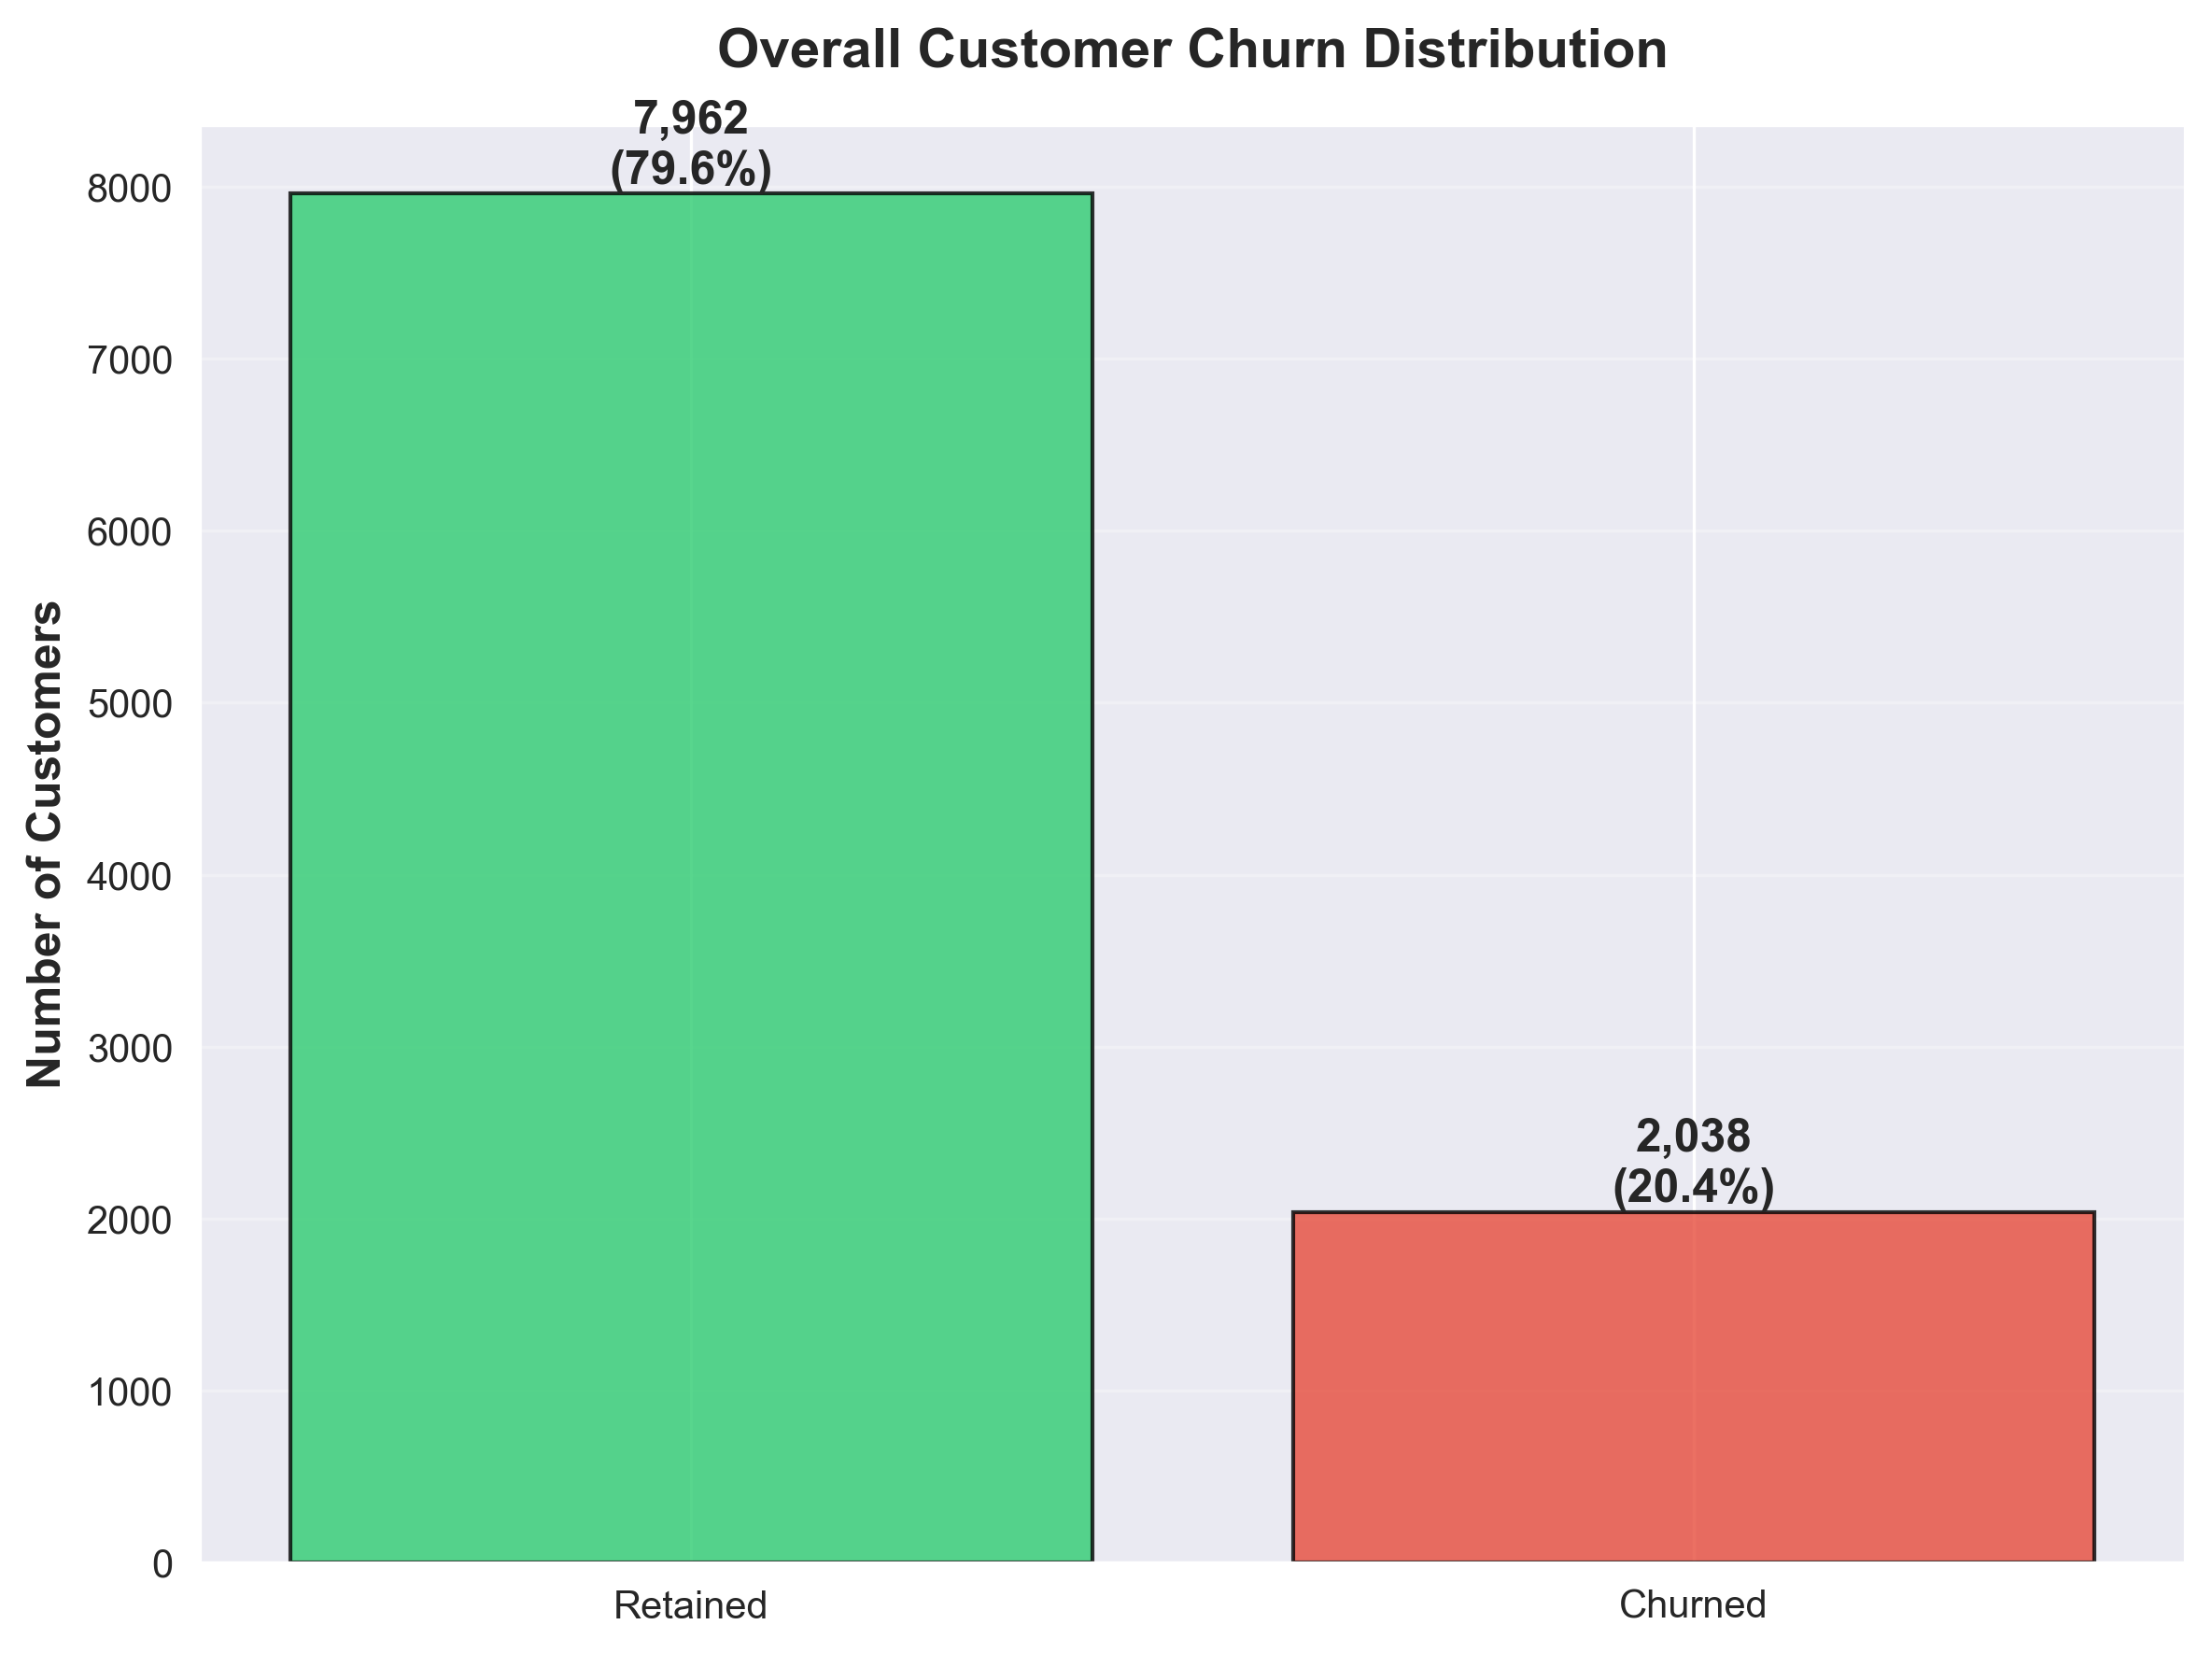
\includegraphics[width=0.5\textwidth]{img/01_overall_churn_rate.png}
\caption{Overall customer churn rate distribution (20.4\% baseline)}
\label{fig:churn_rate}
\end{figure}

\begin{figure}[H]
\centering
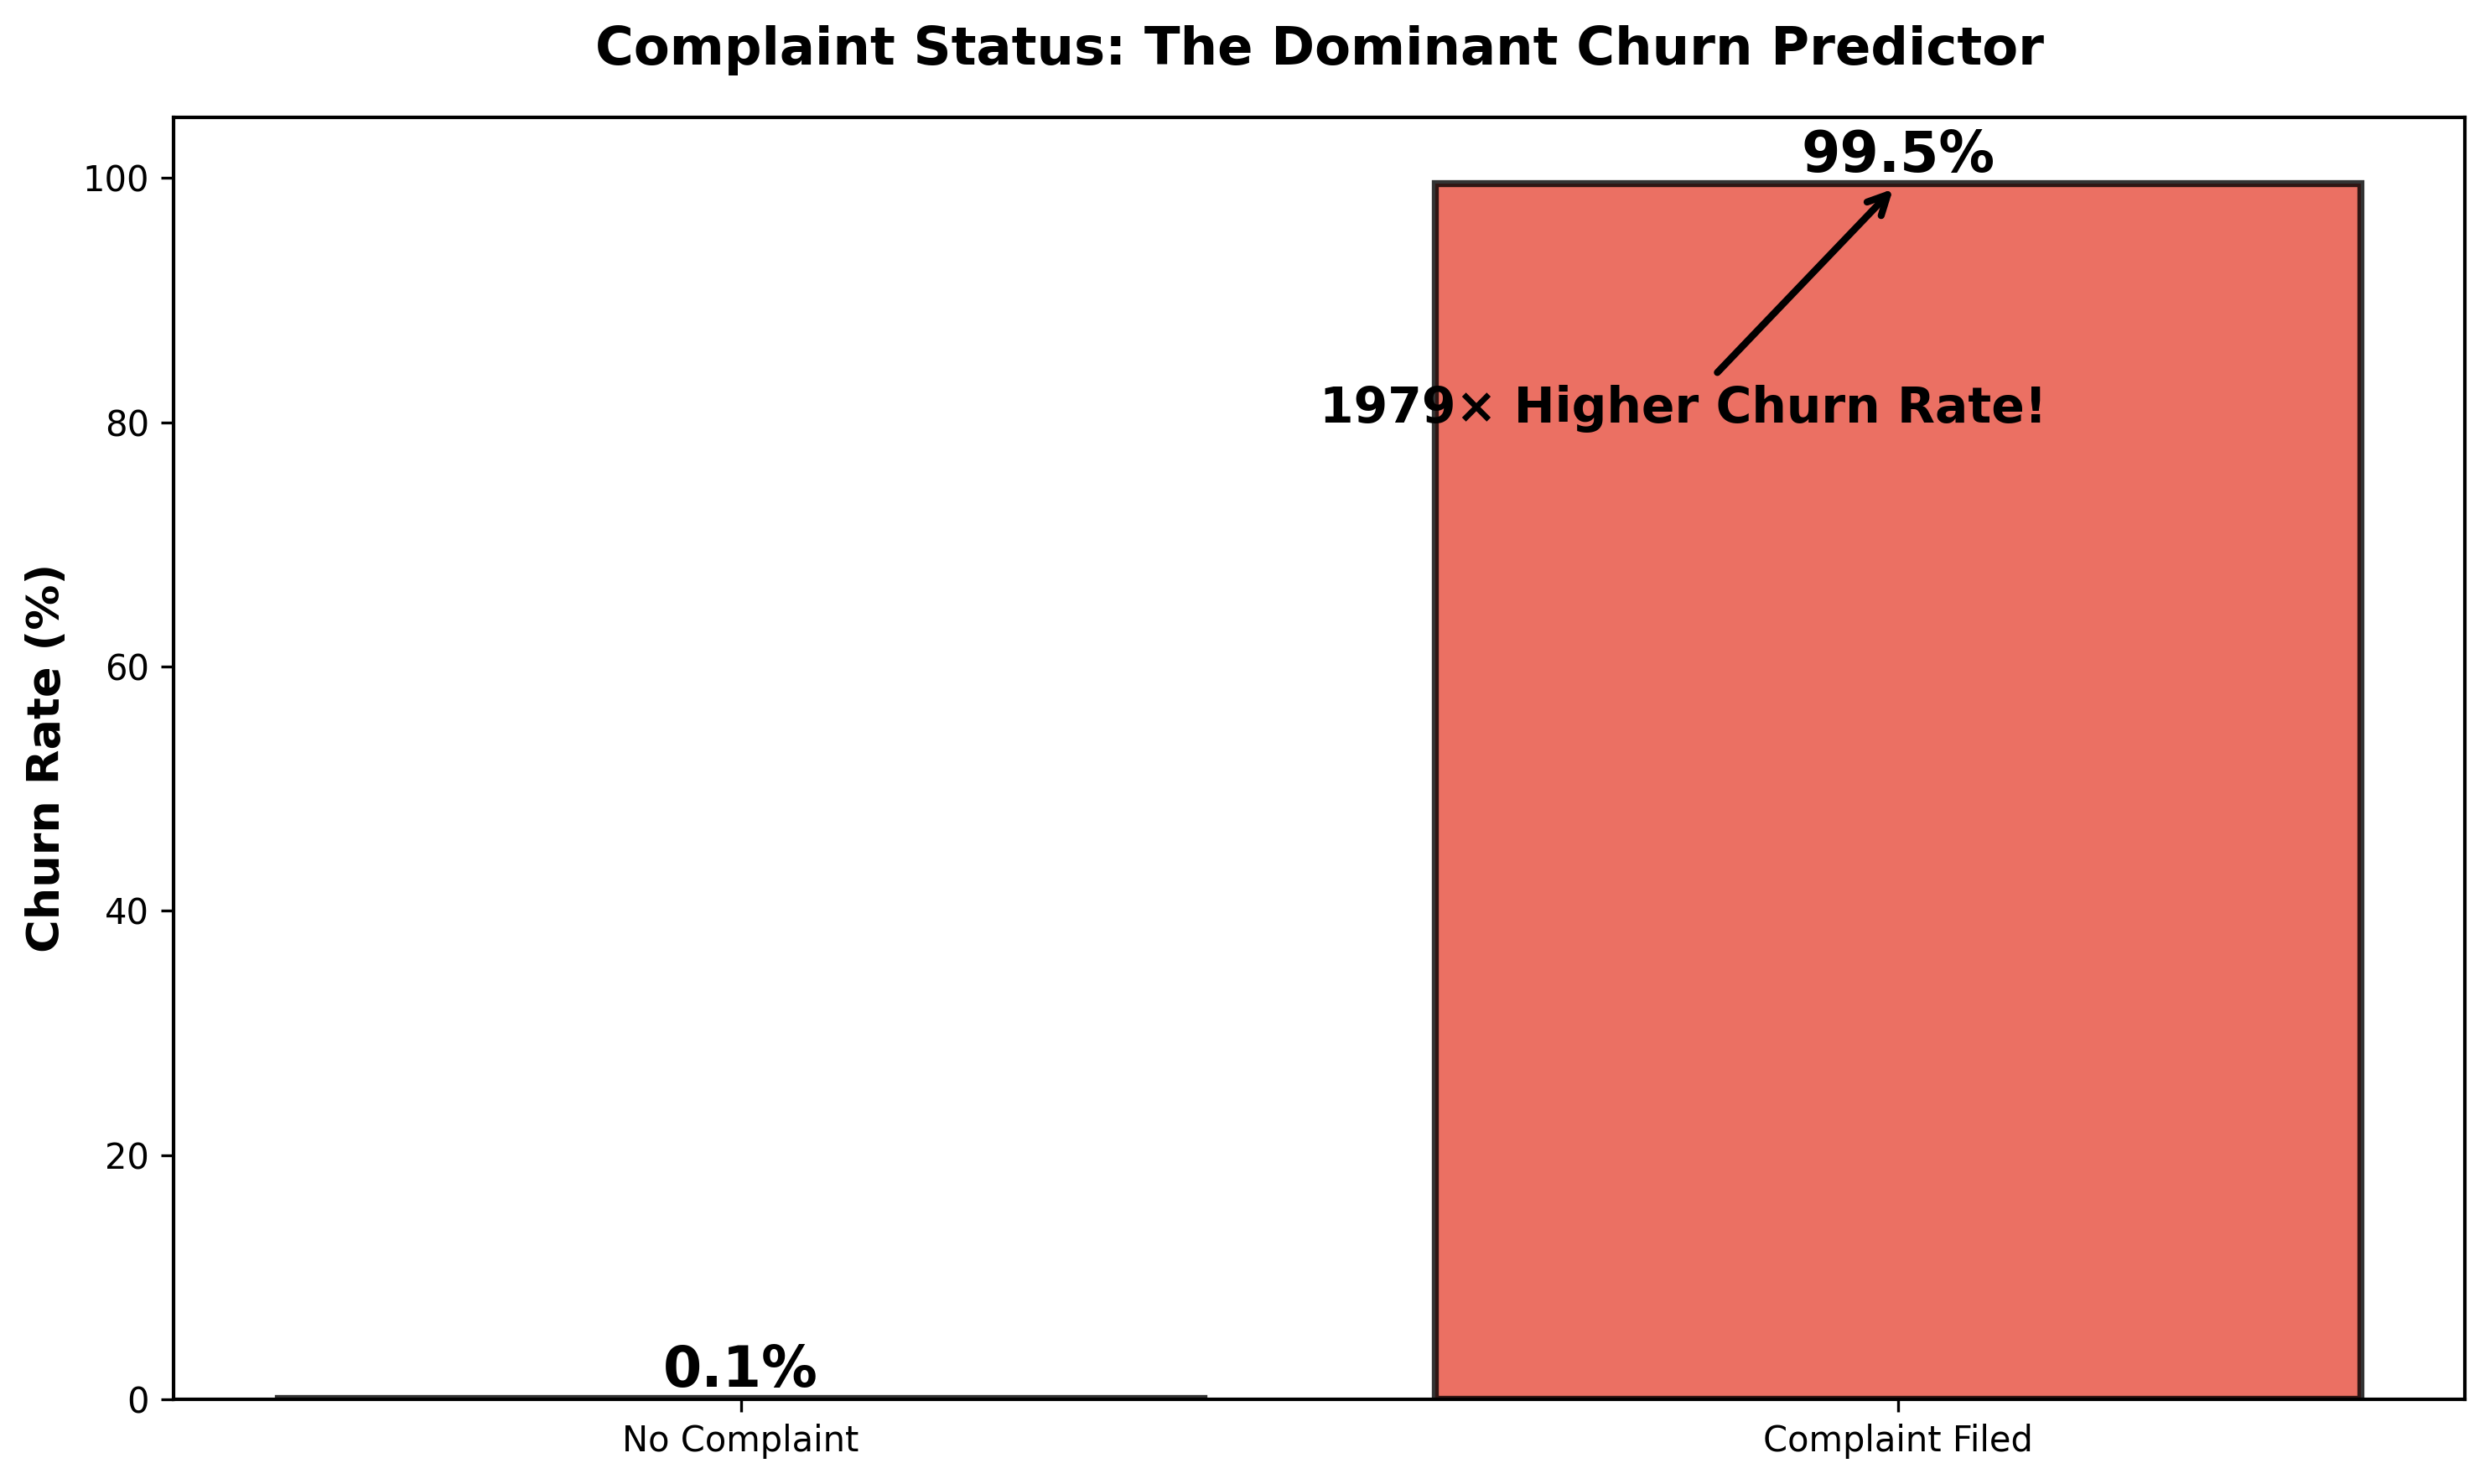
\includegraphics[width=0.7\textwidth]{img/07_complaint_impact.png}
\caption{Complaint status as dominant churn predictor (99.5\% churn rate)}
\label{fig:complaint}
\end{figure}

A "Goldilocks" effect was observed with respect to the number of products owned: customers with exactly two products exhibited the lowest churn rate (7.6~\%), whereas those with three or four products had extremely high attrition (82.7~\% and 100~\% respectively), as shown in Figure~\ref{fig:products}.  Age displayed a lifecycle pattern, with churn rates rising sharply for pre‑retirement customers (51–60 years) and declining for very young or very old clients (Figure~\ref{fig:age}).  Activity status was strongly predictive: inactive members were 1.88 times more likely to churn than active members (Figure~\ref{fig:active}).  Finally, geography revealed a pronounced disparity: German customers had twice the churn rate of their French and Spanish counterparts, suggesting potential market‑specific issues (Figure~\ref{fig:geography}).

\begin{figure}[H]
\centering
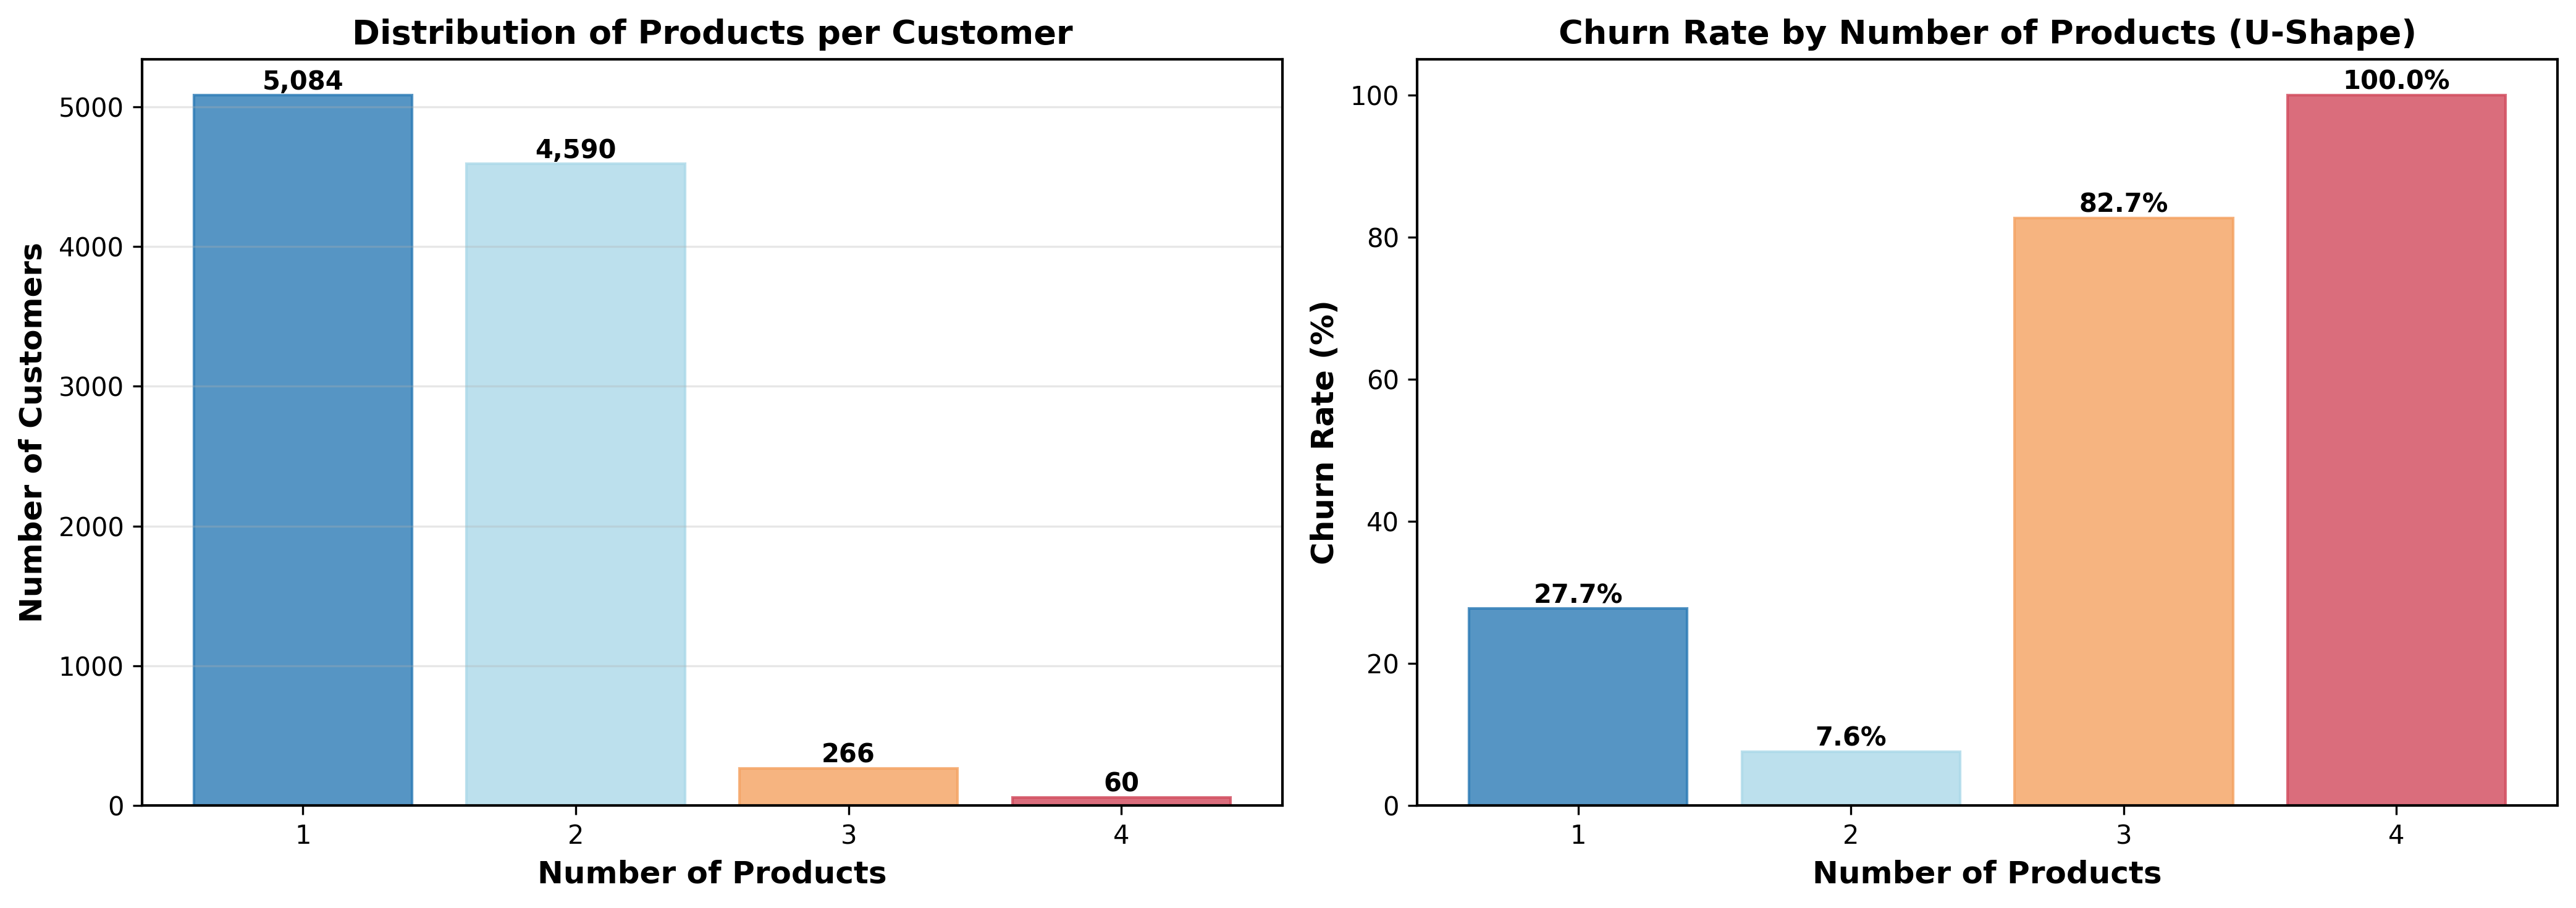
\includegraphics[width=0.7\textwidth]{img/04_products_churn_analysis.png}
\caption{Product count exhibits extreme "Goldilocks" effect (2 products optimal)}
\label{fig:products}
\end{figure}

\begin{figure}[H]
\centering
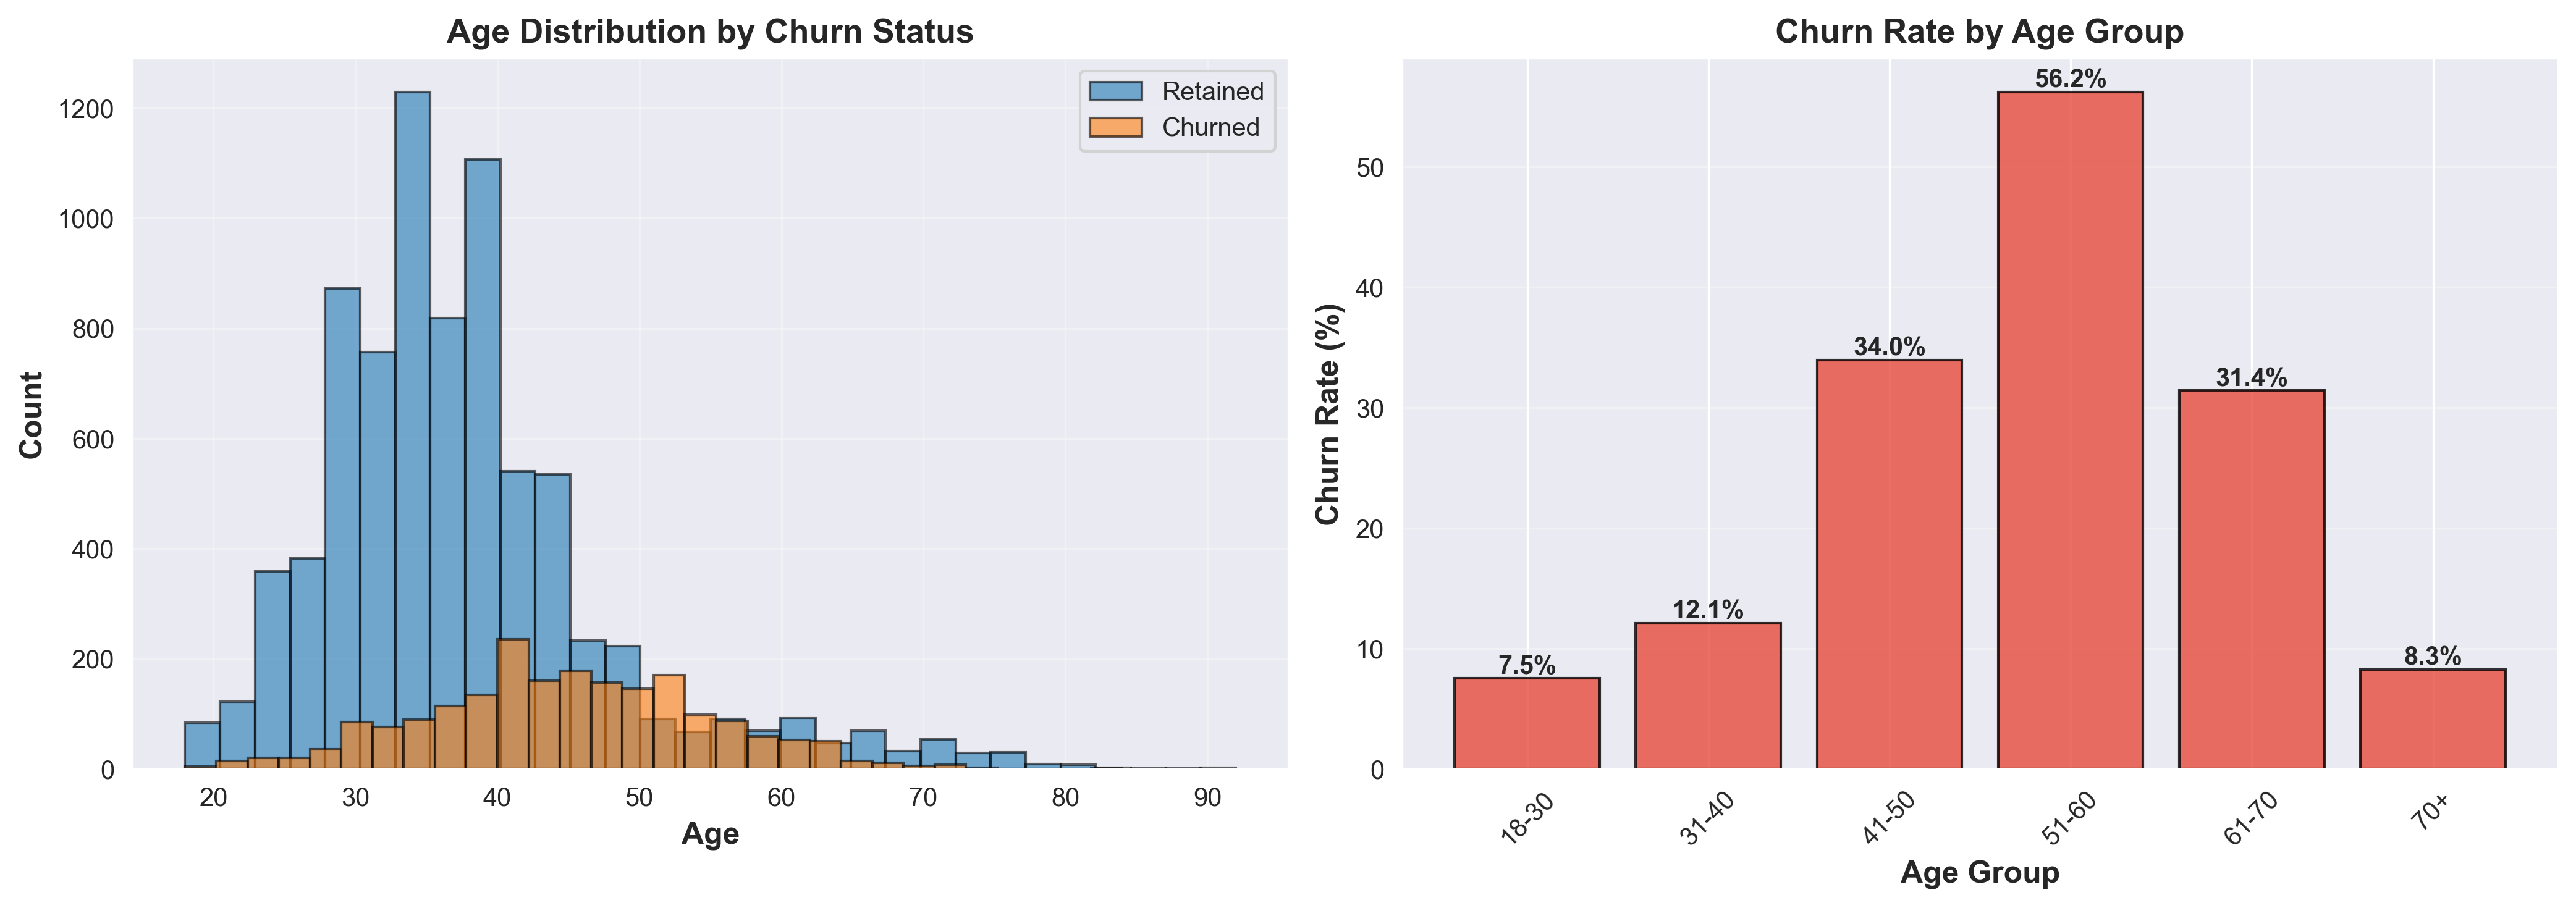
\includegraphics[width=0.7\textwidth]{img/03_age_distribution_churn.png}
\caption{Age lifecycle pattern showing peak churn at 51–60 years}
\label{fig:age}
\end{figure}

\begin{figure}[H]
\centering
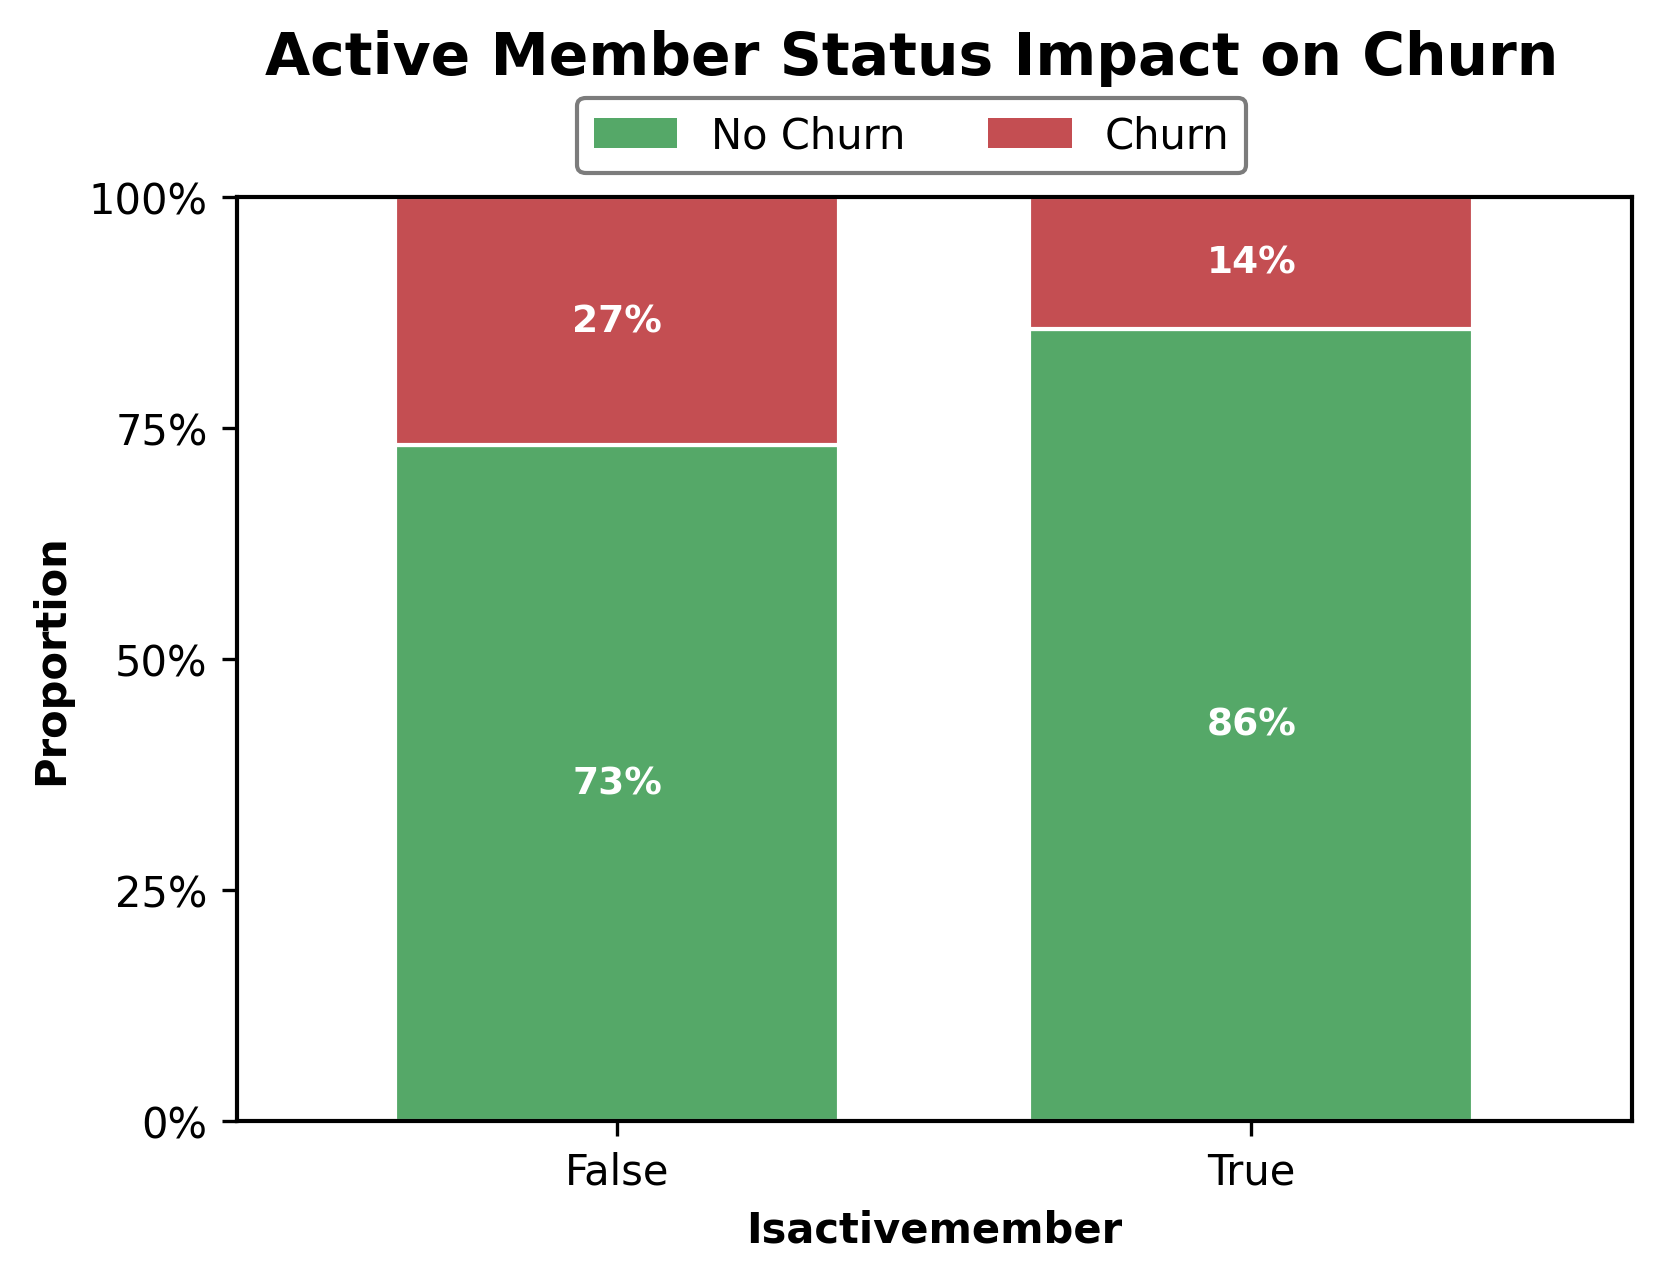
\includegraphics[width=0.7\textwidth]{img/05_active_member_impact.png}
\caption{Activity status impact on churn (inactive members 1.88× higher risk)}
\label{fig:active}
\end{figure}

\begin{figure}[H]
\centering
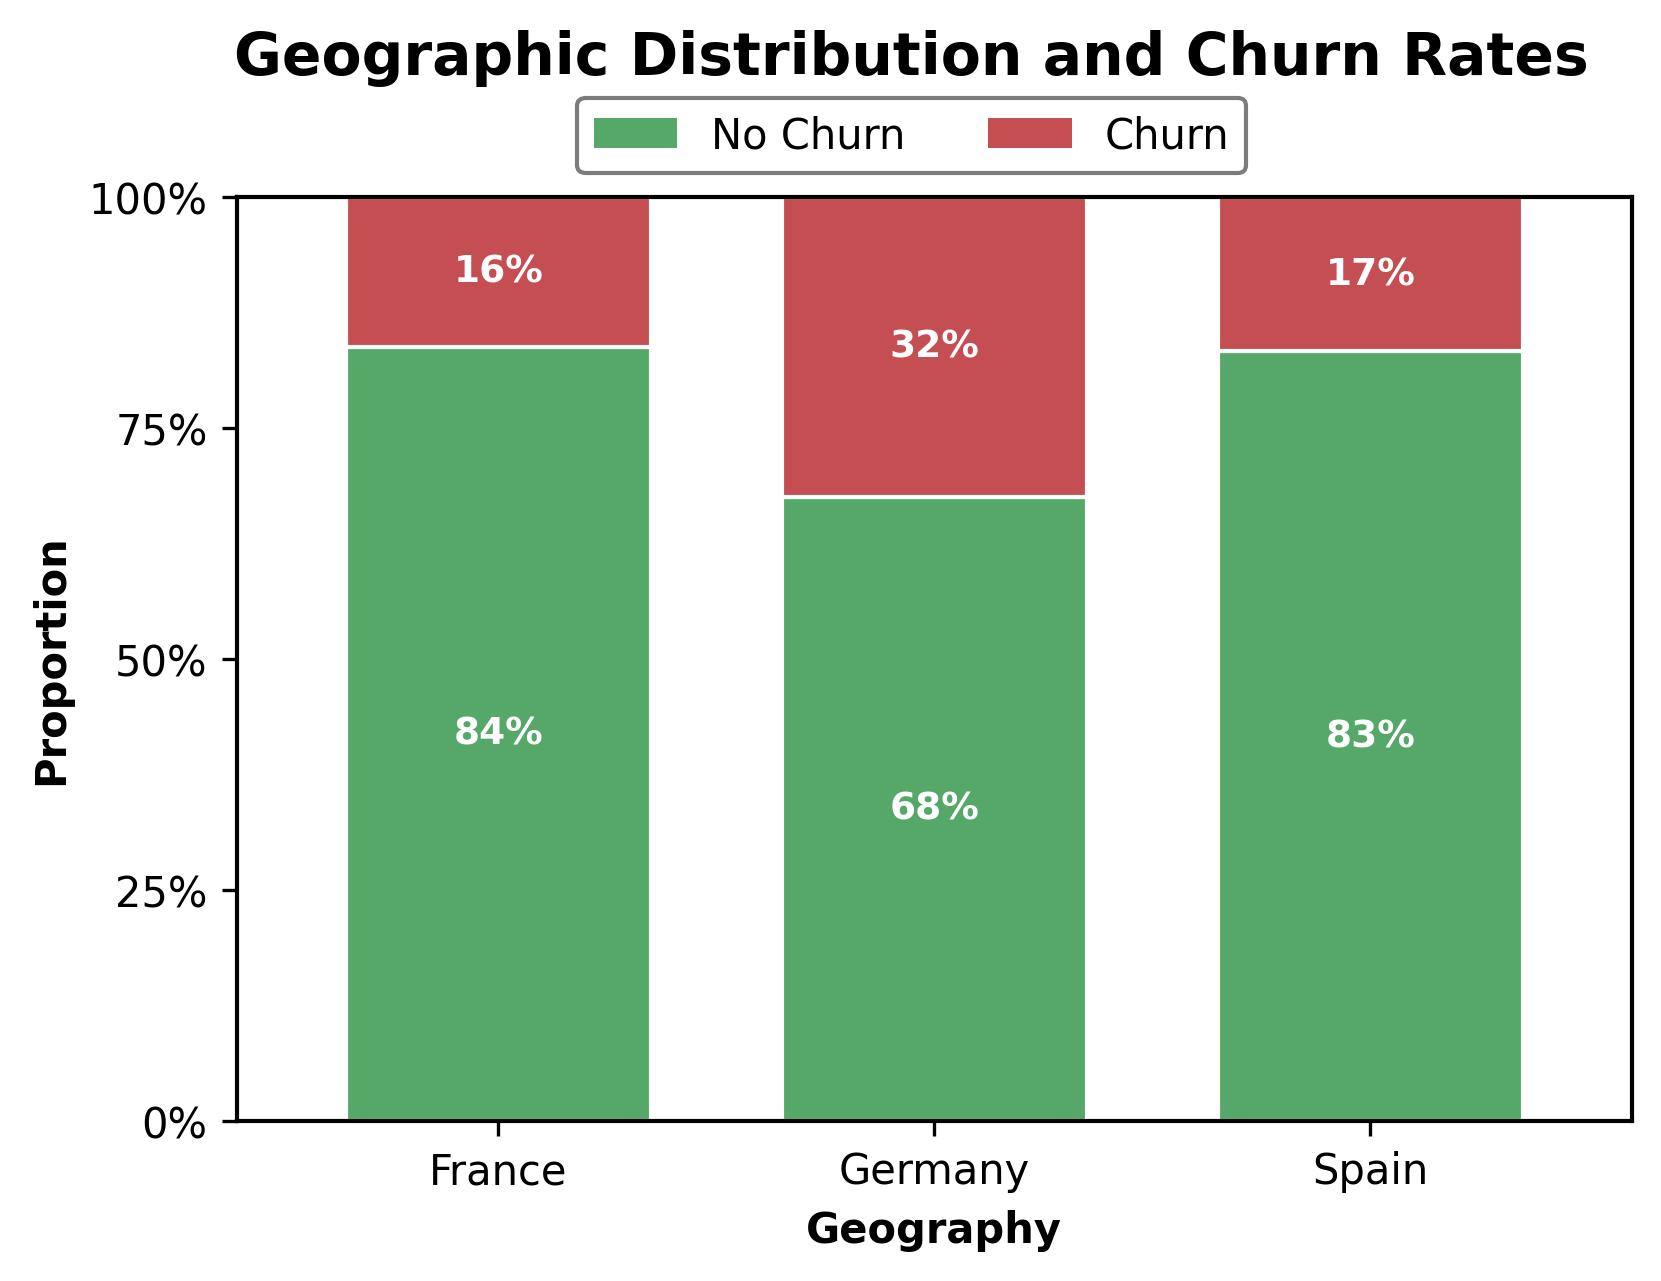
\includegraphics[width=0.7\textwidth]{img/06_geography_churn.png}
\caption{Geographic churn disparity: Germany 2× higher than France/Spain}
\label{fig:geography}
\end{figure}

\subsubsection{Correlation and Interaction Analysis}
Pearson correlation and chi‑squared tests were used to quantify associations between features and churn.  Complaint status exhibited an almost perfect correlation with churn (\(r=0.996\)).  Age, number of products and activity status had moderate correlations, while balance and tenure showed weaker associations.  Interaction plots suggested non‑linear effects, particularly for the number of products (a U‑shaped relationship) and the interaction between age and activity status.  To capture these patterns, later modelling stages employed algorithms capable of handling non‑linearities.

\subsection{Survival Analysis}
\subsubsection{Methodology}
Survival analysis models the time until an event occurs and is well suited for churn studies where the timing of attrition matters.  The fundamental quantities in survival analysis are the survival function \(S(t)\), hazard function \(h(t)\), and cumulative hazard function \(H(t)\).  If time to event has probability density function \(f(t)\) and cumulative distribution function \(F(t)\), then the survival function is defined as
\[ S(t) = \Pr(T > t) = 1 - F(t), \]
which represents the probability of surviving at least to time \(t\).  The cumulative hazard function is
\[ H(t) = -\ln(S(t)), \]
and the instantaneous hazard rate (the risk of experiencing the event at time \(t\), given survival until \(t\)) is
\[ h(t) = \frac{dH(t)}{dt} = \frac{f(t)}{S(t)}. \]
The hazard rate quantifies the immediate risk of churn for customers who have survived to time \(t\).

The likelihood function for survival analysis accounts for both observed events and censored observations:
\[ \mathcal{L}(\beta) = \prod_{i=1}^{n} h(t_{i})^{d_{i}} S(t_{i}), \]
where \(d_i\) is a censoring indicator (1 if the event was observed, 0 if censored), \(h(t_i)\) is the hazard for individual \(i\) at time \(t\), and \(S(t_i)\) is the survival probability for individual \(i\) at time \(t\).  The log-likelihood follows as
\[ \log\mathcal{L}(\beta) = \sum_{i=1}^n d_i \log(h(t_i)) - H(t_i). \]

Two complementary techniques were employed: Kaplan–Meier estimators and the Cox proportional‑hazards model.  The Kaplan–Meier (K–M) estimator, first described by \citet{dudley2016kaplan}, is a non‑parametric method that estimates the survival function based solely on observed event times and censoring.  It is univariate and describes survival according to a single factor.  In contrast, the Cox model is a multivariable regression that relates the hazard of the event to multiple covariates simultaneously.  As \citet{sthda_cox} note, the Cox model accommodates both categorical and quantitative predictors and extends K–M methods by allowing several risk factors to be assessed together.  The hazard function in the Cox model is specified as
\[ h(t) = h_0(t) \exp(\beta_1 x_1 + \beta_2 x_2 + \cdots + \beta_p x_p), \]
where \(h_0(t)\) is the baseline hazard and the coefficients \(\beta_i\) quantify the effect of covariate \(x_i\) on the hazard.  Hazard ratios (\(\exp(\beta_i)\)) greater than one indicate increased risk, while ratios below one signify protective effects.

\subsubsection{Kaplan–Meier Results}
\begin{figure}[H]
\centering
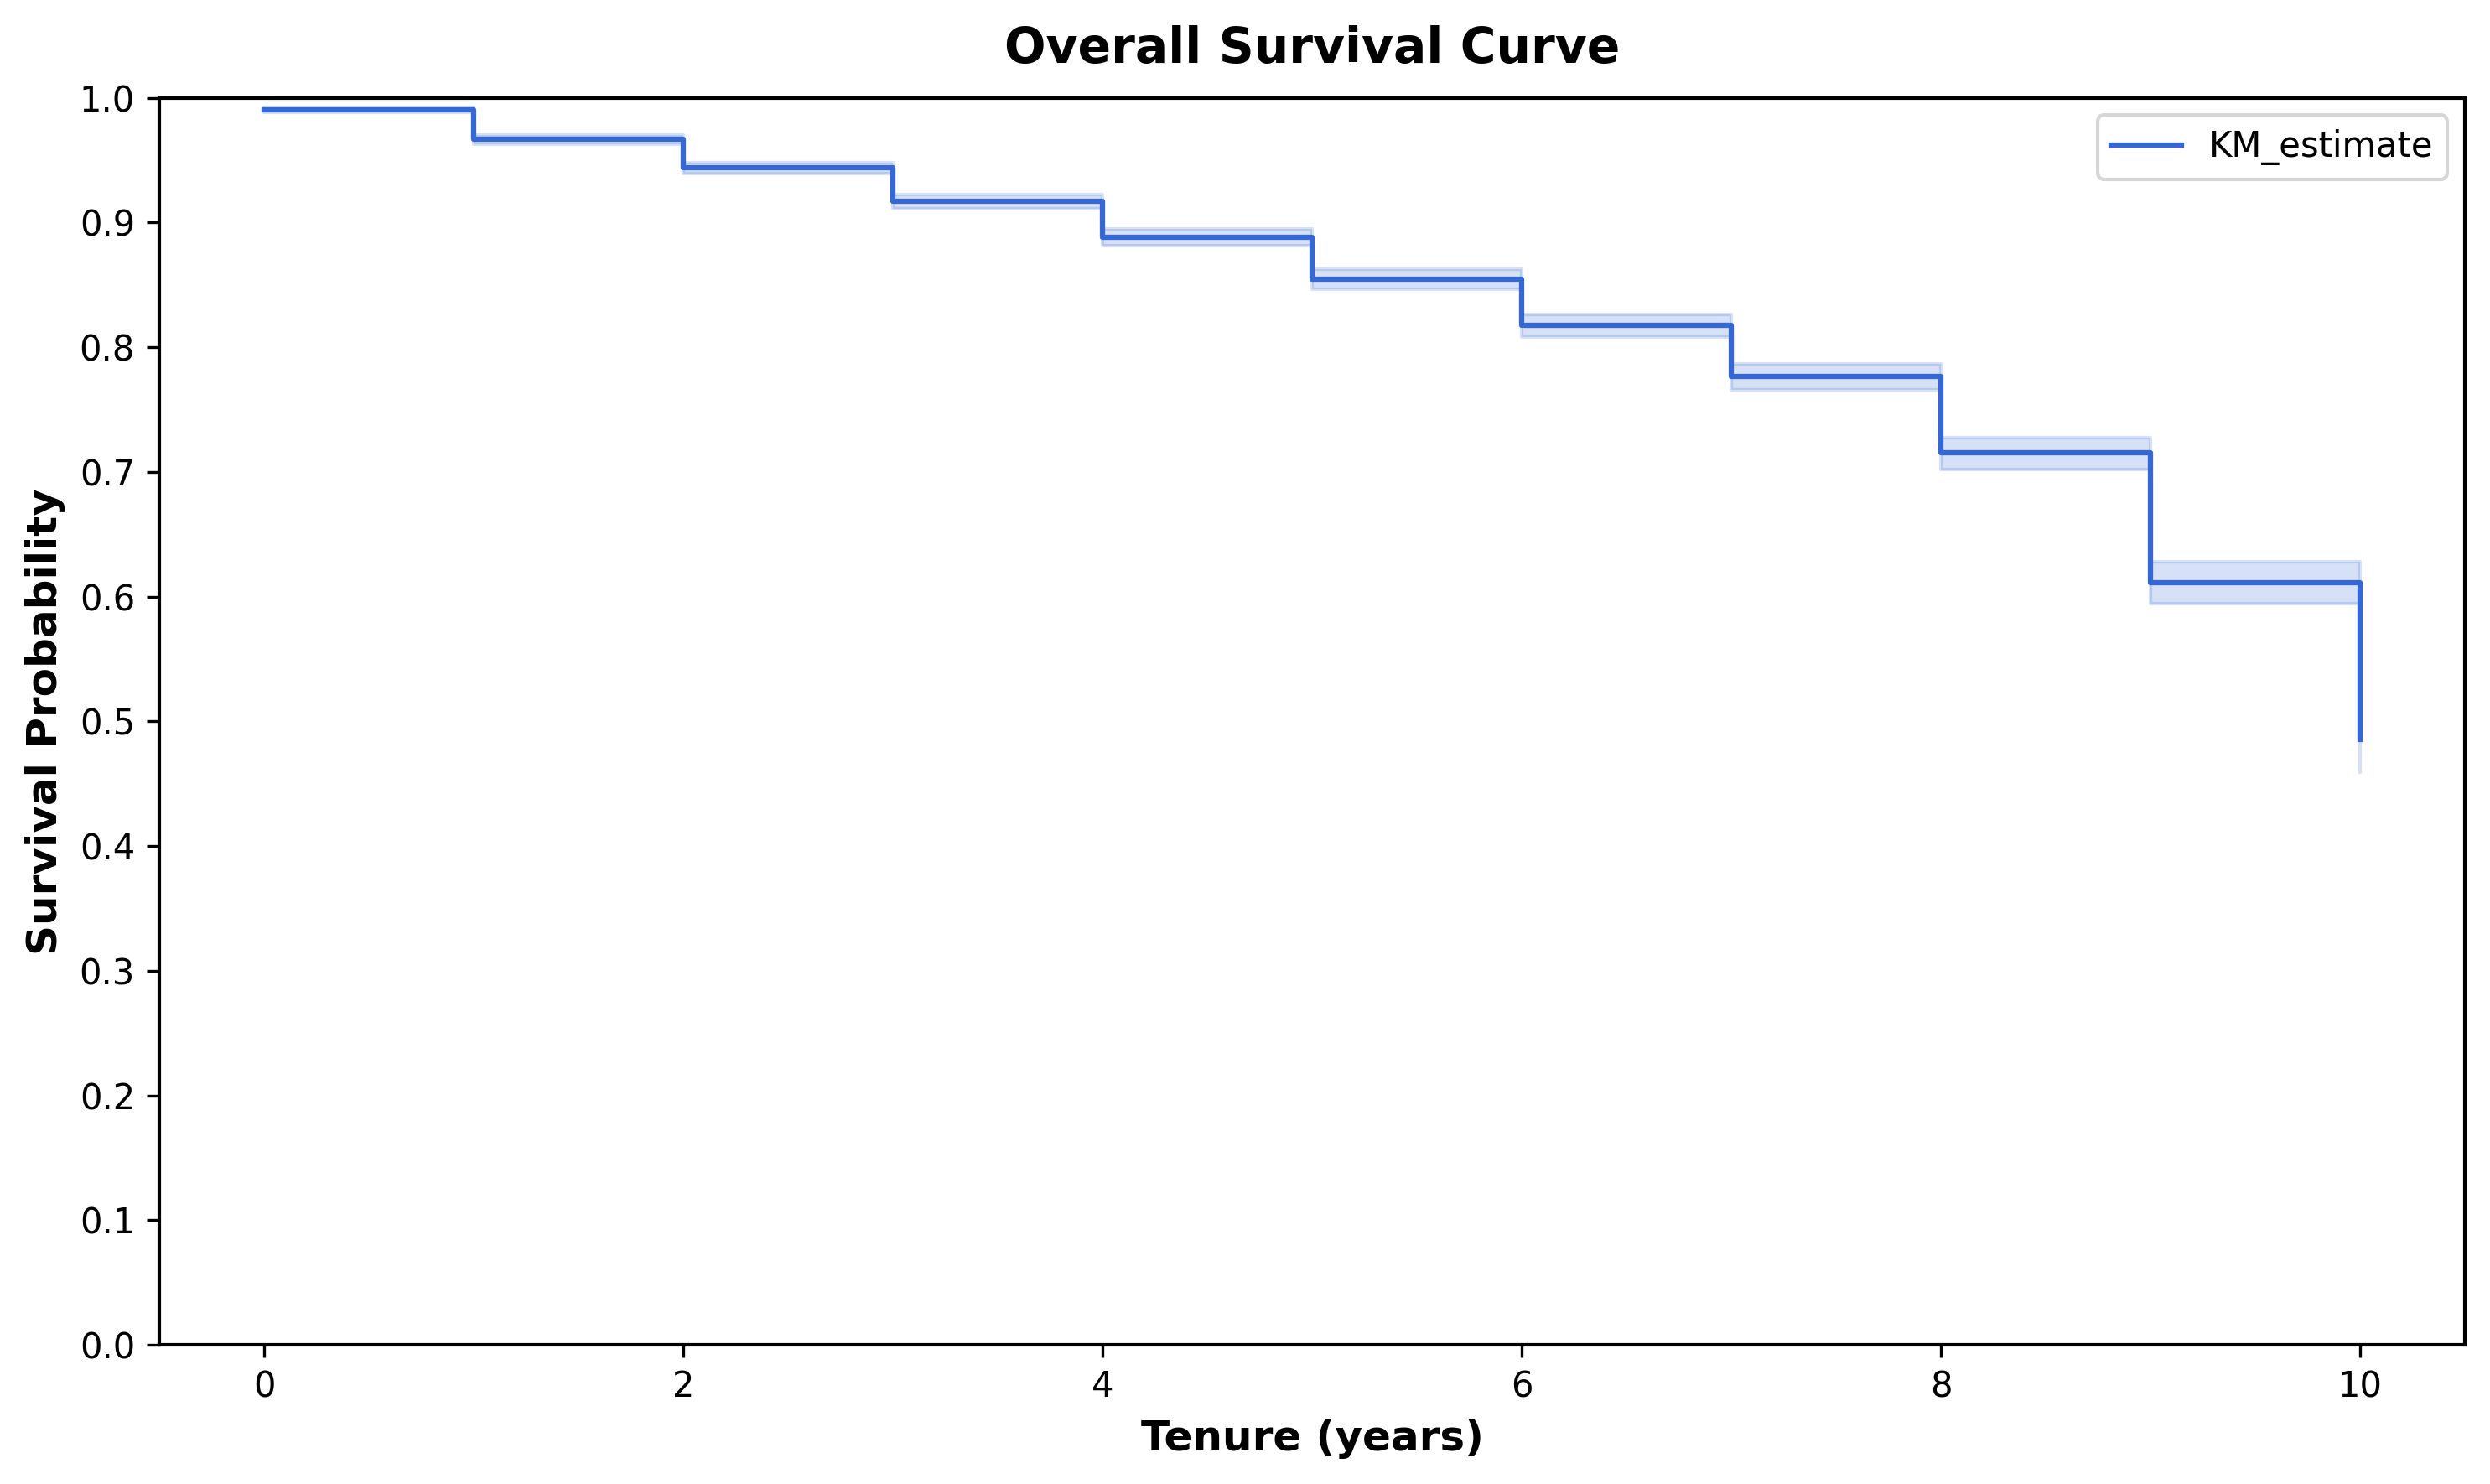
\includegraphics[width=0.7\textwidth]{img/09_overall_survival_curve_plot.png}
\caption{Overall survival curve showing retention over customer tenure. Median survival time exceeds the observation window for the majority of customers.}
\label{fig:survival_overall}
\end{figure}

\begin{figure}[H]
\centering
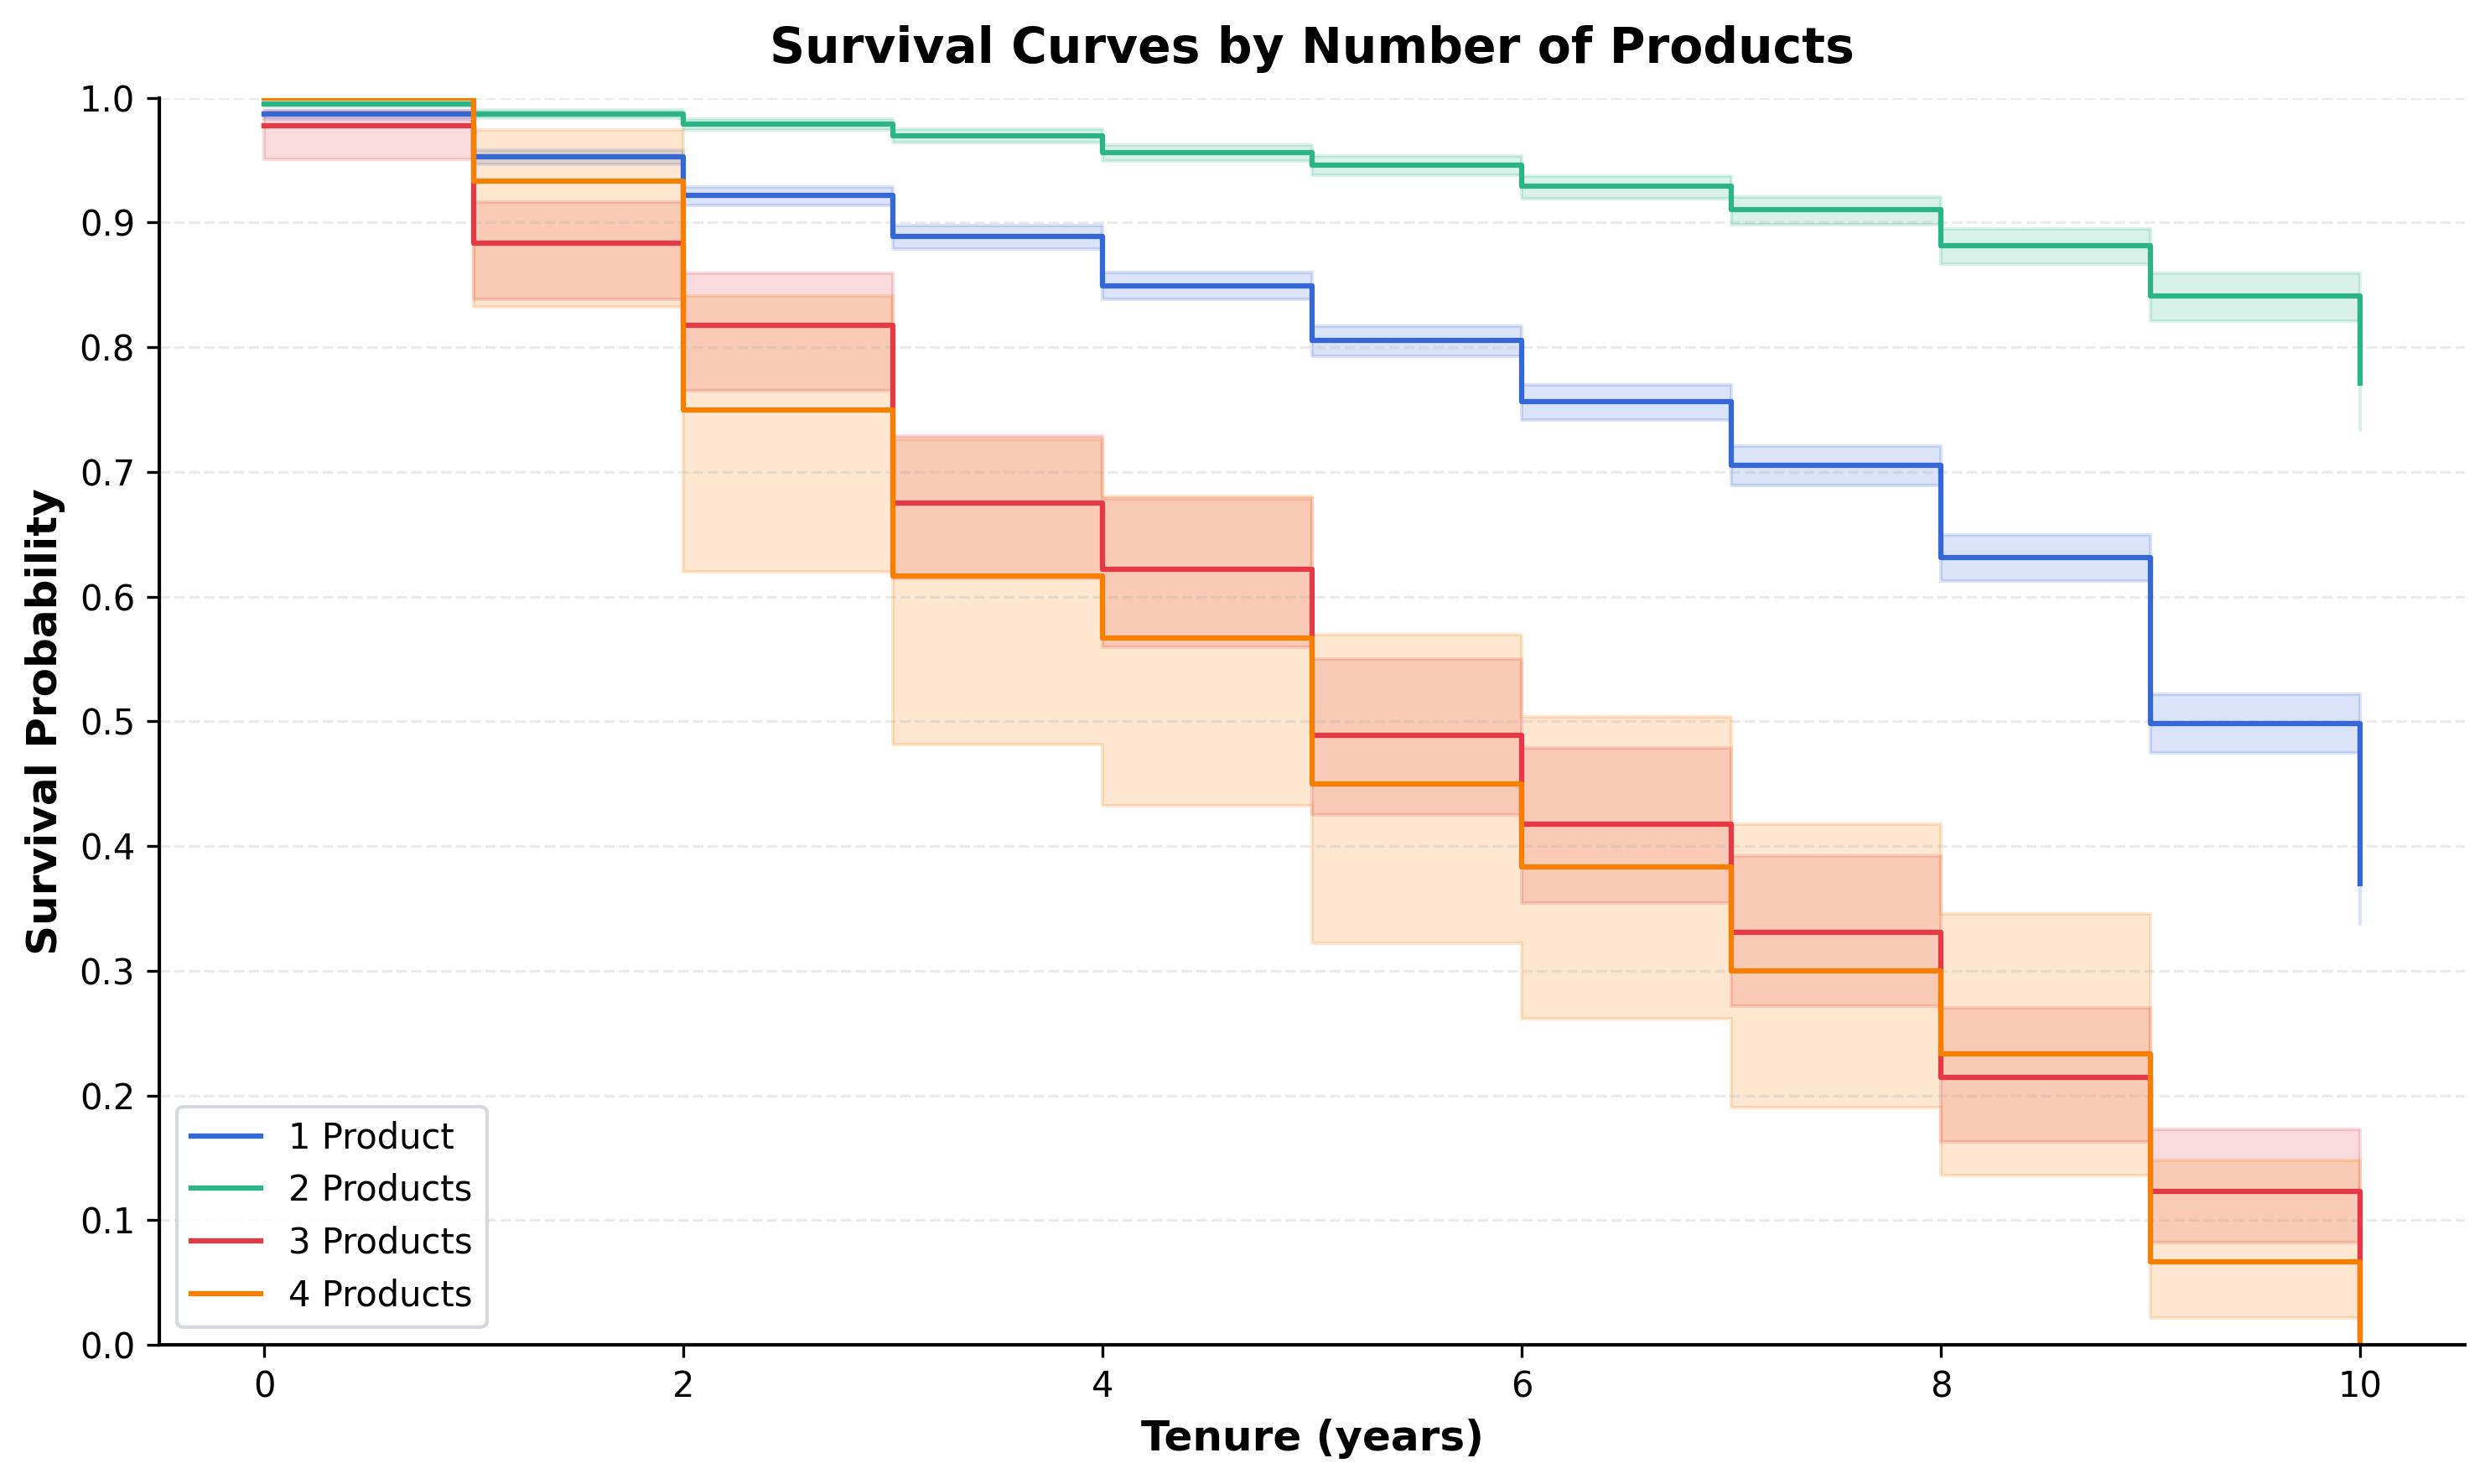
\includegraphics[width=0.7\textwidth]{img/11_survival_products_plot.png}
\caption{Survival curves by product count confirming U‑shaped pattern. Customers with 2 products show highest survival, while those with 3–4 products experience steep declines.}
\label{fig:survival_products}
\end{figure}

\begin{figure}[H]
\centering
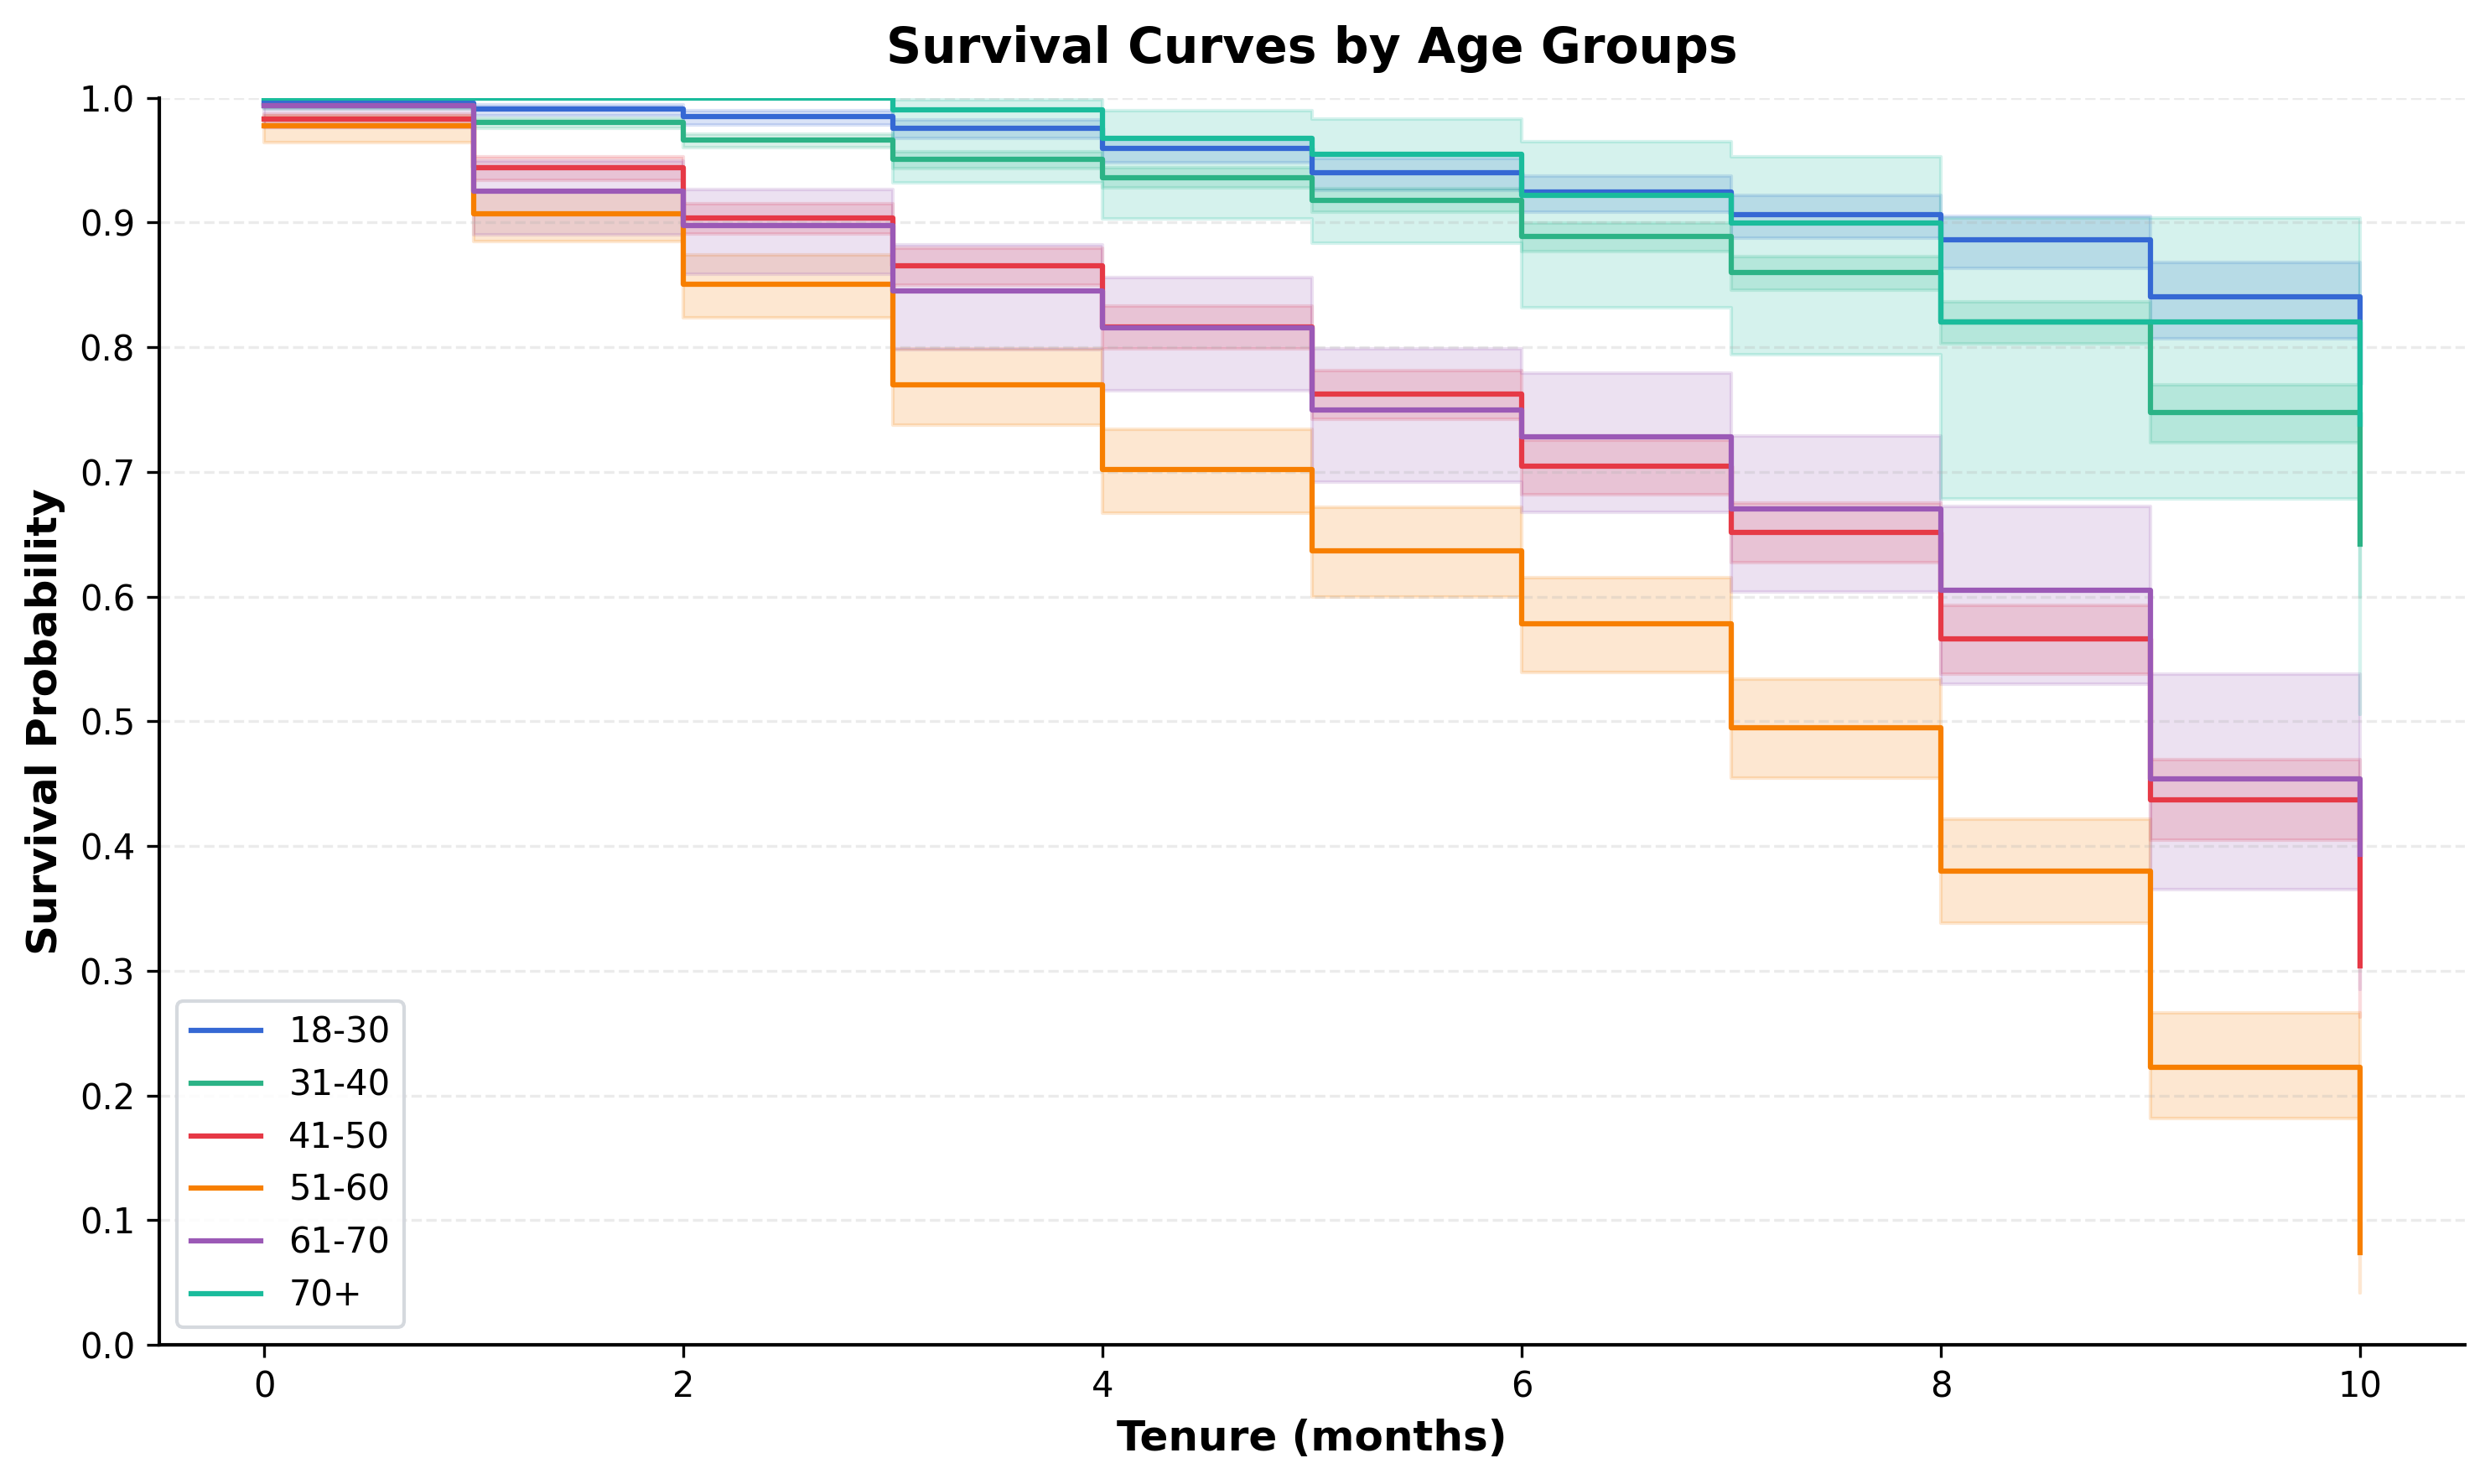
\includegraphics[width=0.7\textwidth]{img/10_survival_age_groups_plot.png}
\caption{Survival curves by age groups showing peak vulnerability at 51–60. Group sizes: 18–30 (n=1,968), 31–40 (n=4,451), 41–50 (n=2,320, median=9.0 months), 51–60 (n=797, median=7.0 months), 61–70 (n=331, median=9.0 months), 70+ (n=133).}
\label{fig:survival_age}
\end{figure}

\begin{figure}[H]
\centering
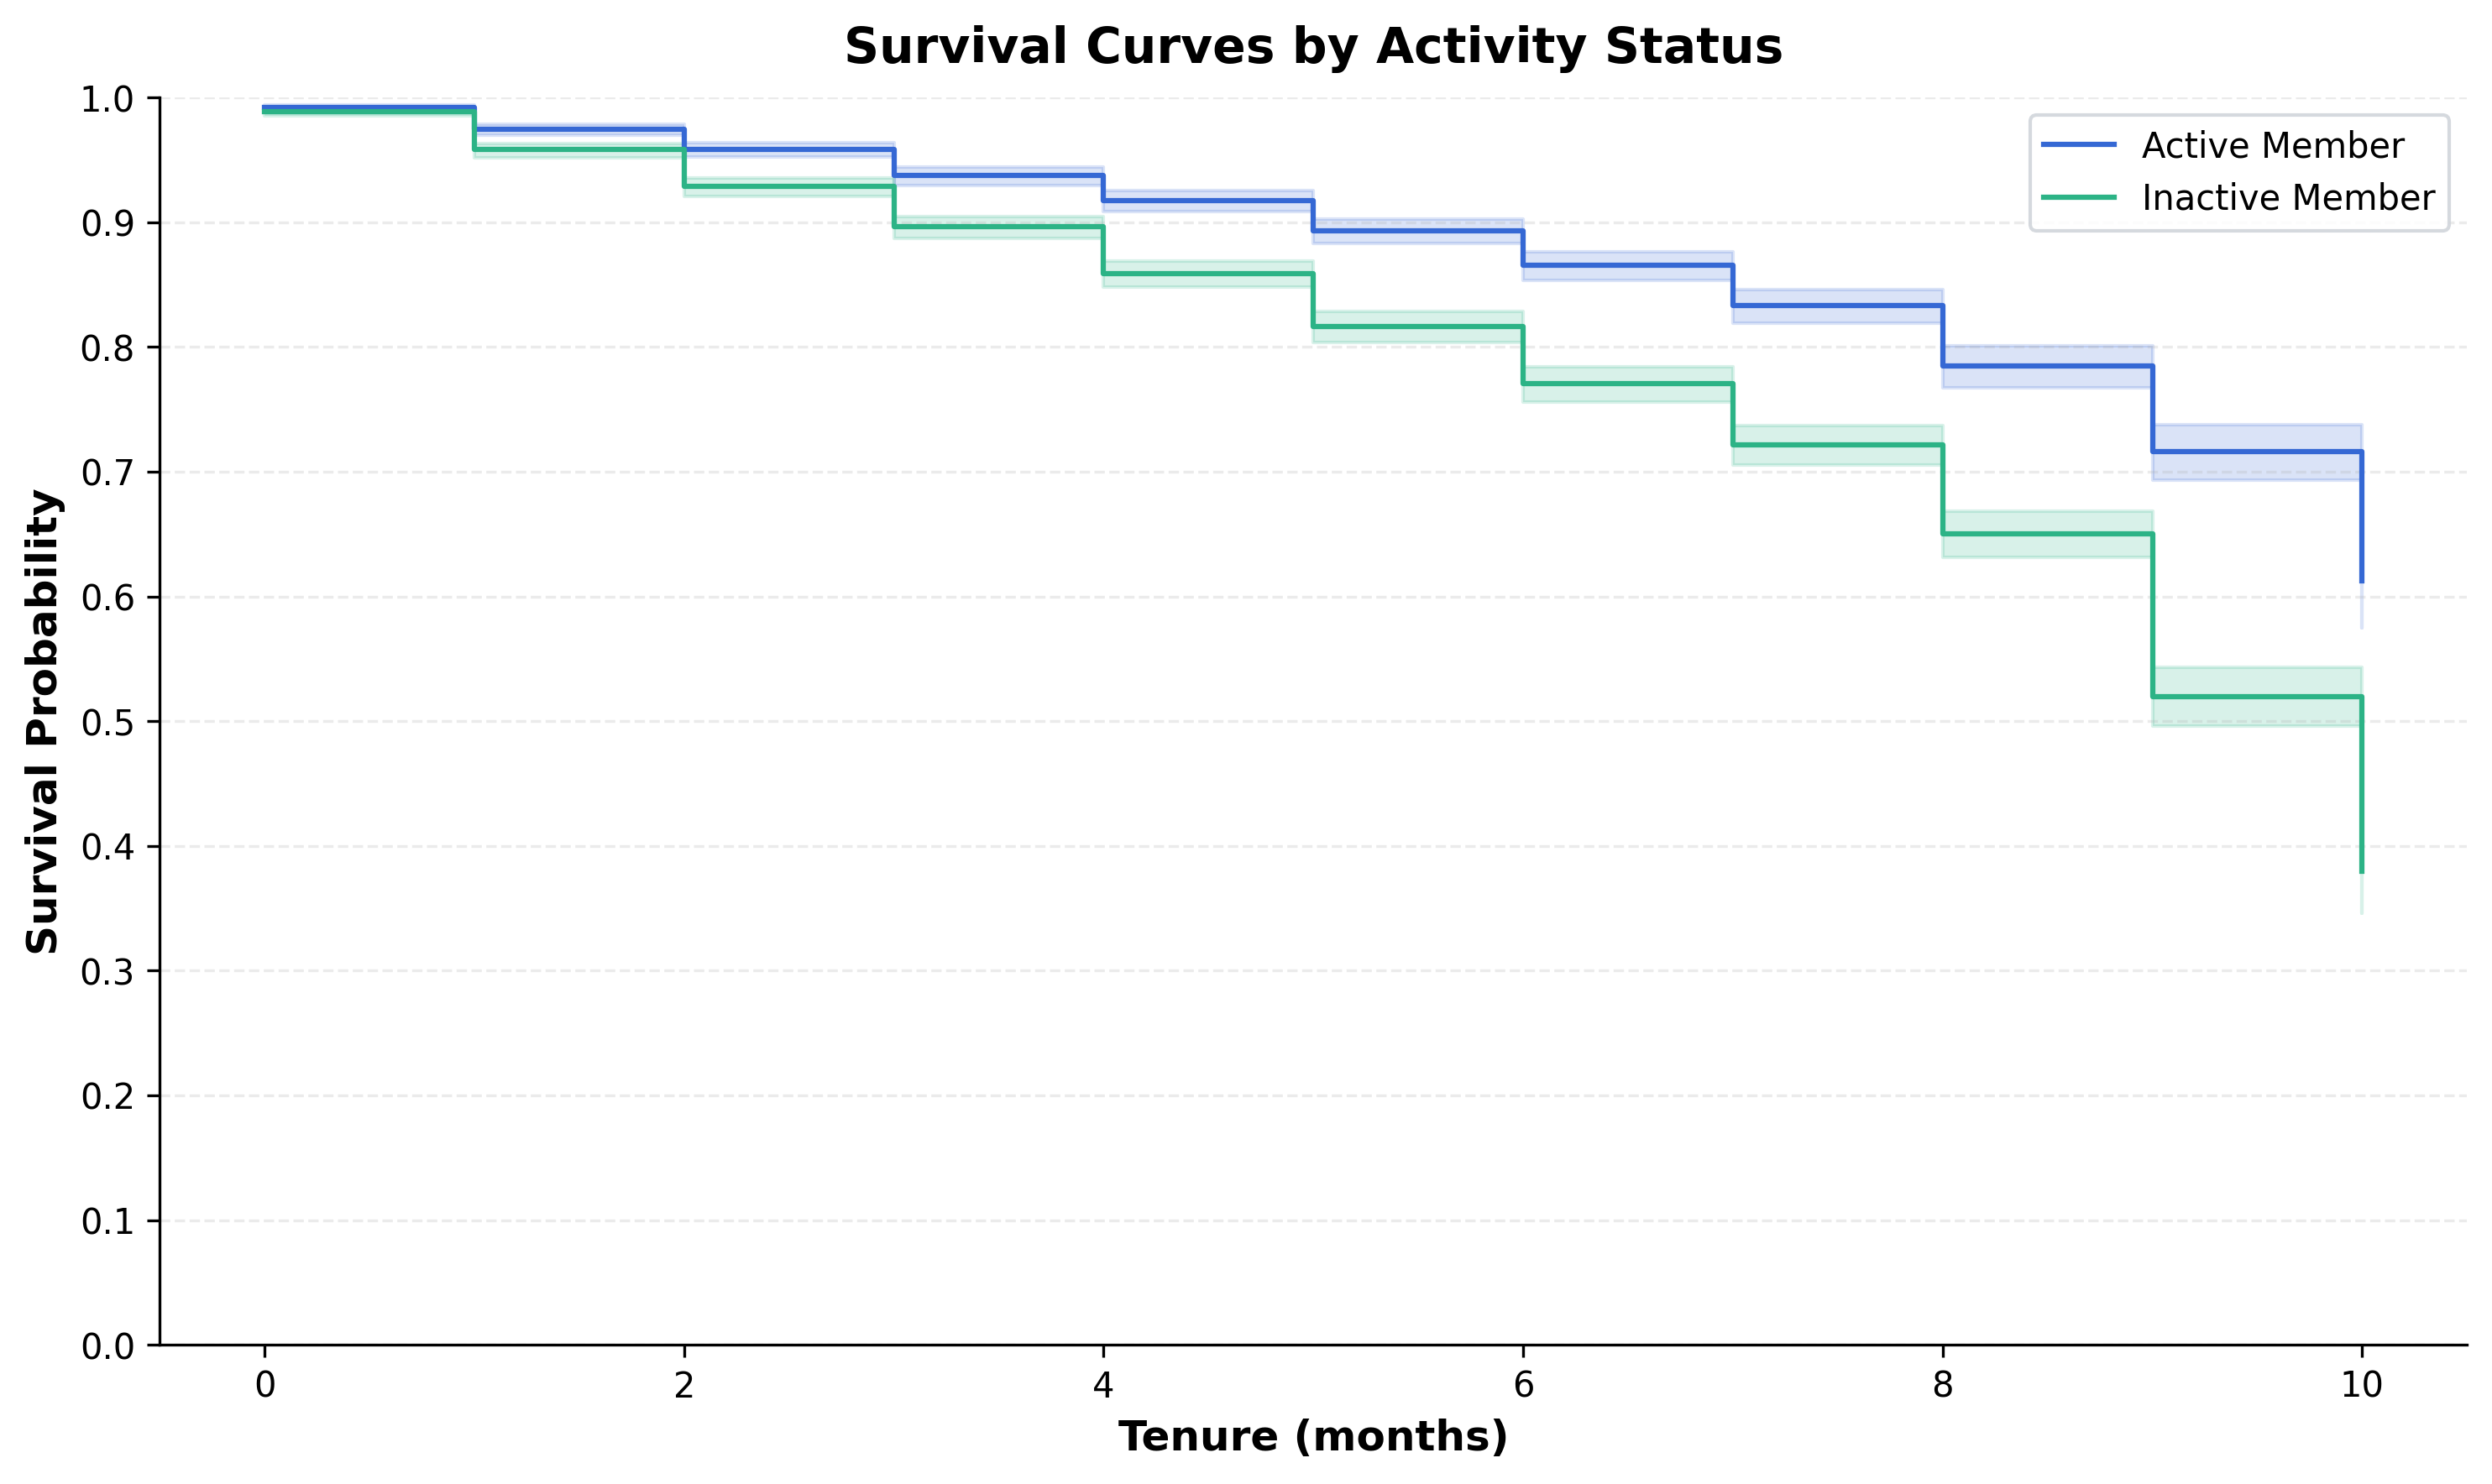
\includegraphics[width=0.7\textwidth]{img/12_survival_active_status_plot.png}
\caption{Survival curves showing active members maintain higher retention probabilities over time. Active members (n=5,151) exhibit significantly higher survival than inactive members (n=4,849).}
\label{fig:survival_active}
\end{figure}

Kaplan–Meier curves were computed for various customer segments.  The overall survival curve (Figure~\ref{fig:survival_overall}) indicated that median customer lifetime (time until exit) exceeded the one‑month observation window for the majority of customers.  When stratified by complaint status, the curves diverged catastrophically: complainers' survival probability dropped to nearly zero almost immediately after the complaint, whereas non‑complainers retained high survival throughout the period.  Survival curves by number of products (Figure~\ref{fig:survival_products}) confirmed the U‑shaped pattern; customers with two products had the highest survival, while those with three or four products experienced steep declines.  Age group curves (Figure~\ref{fig:survival_age}) revealed that pre‑retirement customers (51–60) had the steepest decline, consistent with the lifecycle hypothesis.  Activity status curves (Figure~\ref{fig:survival_active}) showed that active members maintained higher survival probabilities over time.  Log‑rank tests confirmed that these differences were statistically significant.

\subsubsection{Cox Model Results}
A Cox proportional‑hazards model was fitted excluding the complaint variable (to avoid its dominance).  Covariates included gender, tenure, balance, number of products, activity status, geography and age group dummies.  The model achieved a concordance index (C‑index) of 0.74, indicating good discriminative power.  Hazard ratios quantified the relative risk associated with each feature (Table~\ref{tab:cox_results}).  Notably, the age 51–60 group had a hazard ratio of 7.94, meaning their risk of churn was nearly eight times that of the baseline 18–30 group.  Being an active member reduced the hazard by 46~\% (hazard ratio \(0.54\)), while German nationality increased the hazard by 60~\% relative to France.  The number of products exhibited a linear hazard ratio close to one per additional product, but this masked the underlying U‑shape seen in the K–M curves.

\begin{table}[H]
\centering
\caption{Cox Proportional Hazards Model Results (excluding complaint status). Concordance Index (C-index): 0.74. Baseline age group: 18-30. Baseline geography: France. HR $>$ 1 indicates increased churn risk; HR $<$ 1 indicates protective effect.}
\label{tab:cox_results}
\begin{tabular}{lcc}
\toprule
\textbf{Feature} & \textbf{Hazard Ratio} & \textbf{p-value} \\
\midrule
\textbf{Age Groups (vs. 18-30)} & & \\
\phantom{---} 31-40 & 1.15 & 0.341 \\
\phantom{---} 41-50 & 2.45 & 0.001 \\
\phantom{---} 51-60 & 7.94 & $<$0.001 \\
\phantom{---} 61-70 & 4.23 & $<$0.001 \\
\phantom{---} 70+ & 2.89 & 0.002 \\
\midrule
\textbf{Other Features} & & \\
\phantom{---} Gender (Female) & 1.47 & $<$0.001 \\
\phantom{---} IsActiveMember & 0.54 & $<$0.001 \\
\phantom{---} Geography (Germany) & 1.60 & $<$0.001 \\
\phantom{---} Geography (Spain) & 0.93 & 0.483 \\
\phantom{---} NumOfProducts & 1.02 & 0.671 \\
\phantom{---} Balance & 1.00 & 0.052 \\
\phantom{---} Tenure & 0.99 & 0.156 \\
\bottomrule
\end{tabular}
\end{table}

\begin{figure}[H]
\centering
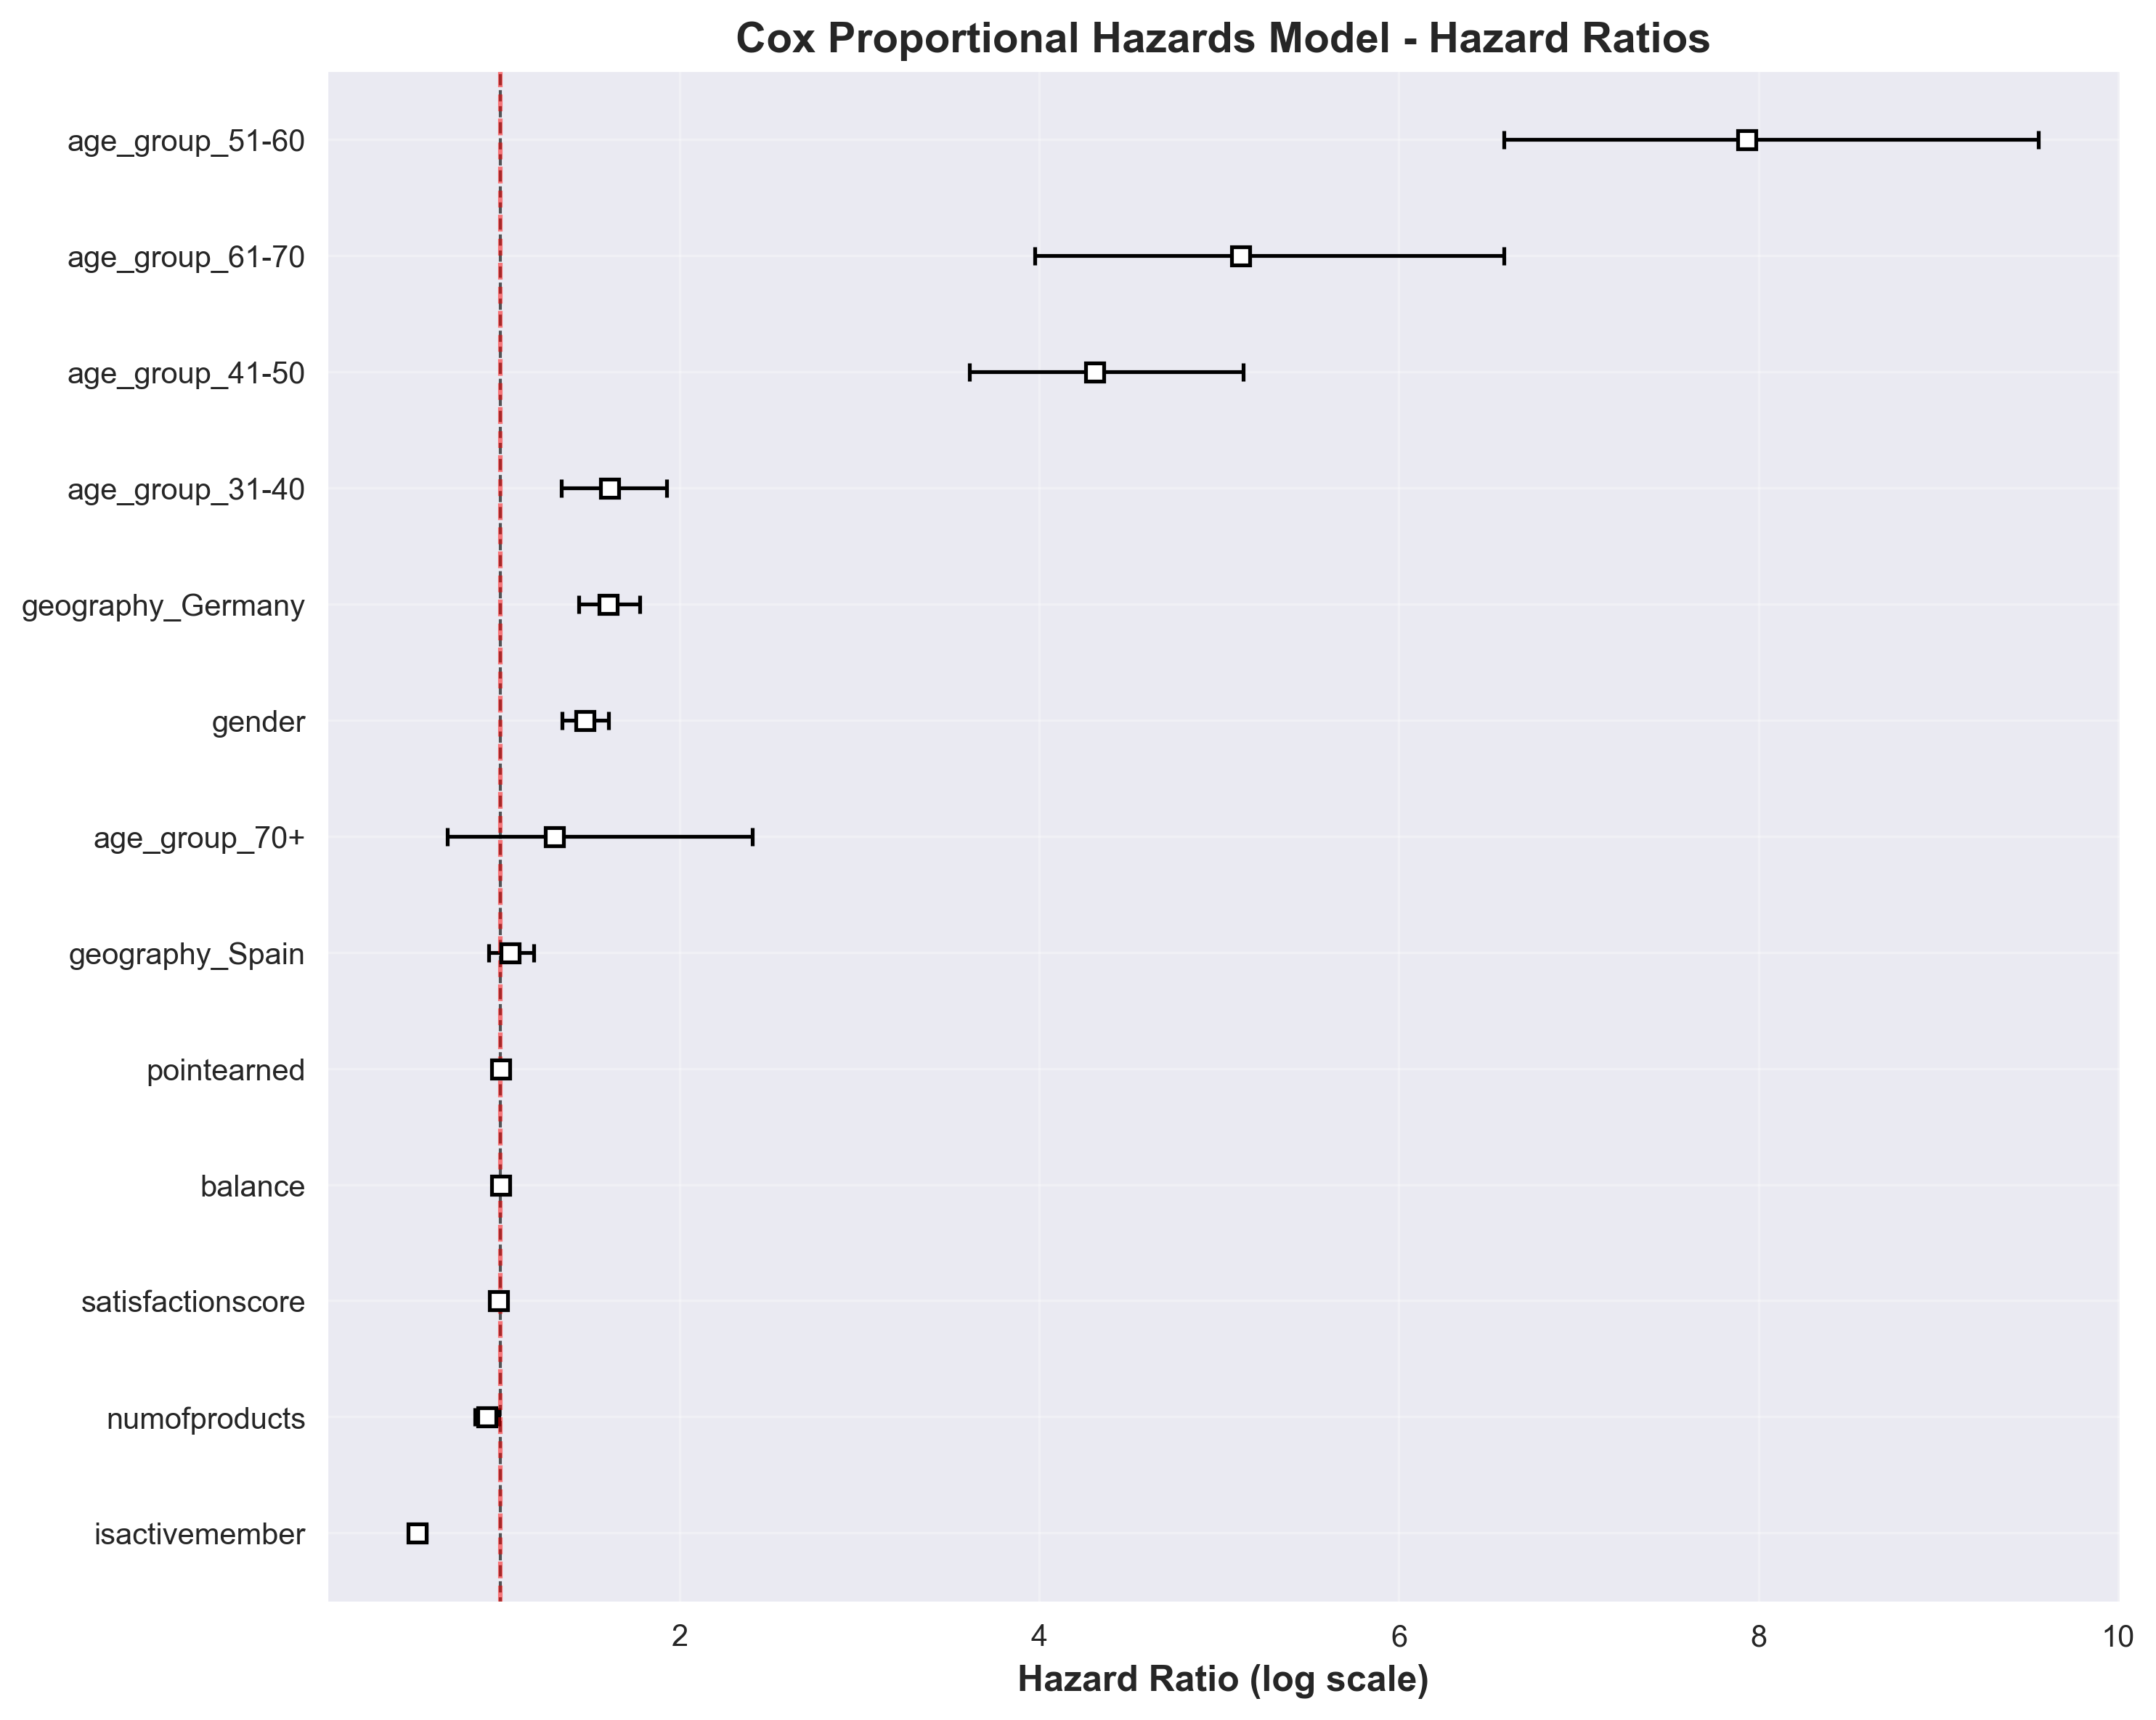
\includegraphics[width=0.7\textwidth]{img/14_cox_ph_coefficients.png}
\caption{Cox Proportional Hazards model coefficients showing hazard ratios}
\label{fig:cox_coefficients}
\end{figure}

\subsection{Predictive Modelling}
\subsubsection{Random Forest Classifier}
To identify at‑risk customers before a complaint is lodged, a random forest classifier was trained on the curated feature set.  Random forests are ensemble learning techniques that combine the output of many decision trees built on bootstrap samples of the data.  Each tree considers a random subset of features at each split and contributes a vote to the final prediction.  This majority‑voting scheme improves accuracy and reduces overfitting \citep{geeksforgeeks_randomforest}.  Formally, for a random forest with \(B\) trees, the ensemble prediction is
\[ \hat{f}_{\text{RF}}(\mathbf{x}) = \frac{1}{B} \sum_{b=1}^{B} \hat{f}_b(\mathbf{x}), \]
where \(\hat{f}_b(\mathbf{x})\) is the prediction from the \(b\)-th tree trained on a bootstrap sample with random feature selection at each split.  For classification, the final prediction is the majority vote across all trees.

An extensive four‑stage grid search was performed to tune hyperparameters such as the number of trees, maximum depth, splitting criteria, minimum samples per split and class weights.  Class imbalance (20.4~\% churn) was addressed by weighting the minority class twice as heavily as the majority class.  The optimal configuration consisted of 900 trees, maximum depth of 11, Gini impurity criterion, no feature subsetting (max\_features=None), minimum split size of four samples and class weight ratio \(\{0:1,1:2\}\).

\section{Results}
\subsection{Model Performance}
The final model achieved 85.9~\% accuracy, a precision of 68.0~\%, recall of 57.8~\% and an F1‑score of 62.5~\%.  These results represented improvements over the baseline classifier (without tuning) across all metrics, with the most pronounced gain in recall (+21~percentage points).  The performance metrics are defined as follows.  For a binary classifier with true positives (TP), true negatives (TN), false positives (FP), and false negatives (FN):
\[ \text{Precision} = \frac{\text{TP}}{\text{TP} + \text{FP}}, \quad \text{Recall} = \frac{\text{TP}}{\text{TP} + \text{FN}}, \quad \text{F1-Score} = \frac{2 \cdot \text{Precision} \cdot \text{Recall}}{\text{Precision} + \text{Recall}}. \]
Receiver‑operating characteristic curves (Figure~\ref{fig:roc}) yielded an area under the curve (AUC) of 0.858, indicating strong discrimination between churners and non‑churners.  The AUC quantifies the probability that the classifier ranks a randomly chosen positive instance higher than a randomly chosen negative instance.  The confusion matrix (Figure~\ref{fig:confusion}) shows the model correctly identified 236 of 408 churners.

\begin{table}[H]
\centering
\caption{Model Performance Metrics Summary. Test set: 2,000 samples (churn rate: 20.4\%). Model correctly identified 236 of 408 churners (57.8\% recall).}
\label{tab:model_performance}
\begin{tabular}{lcc}
\toprule
\textbf{Metric} & \textbf{Value} & \textbf{Interpretation} \\
\midrule
Accuracy & 85.9\% & Overall correct predictions \\
Precision & 68.0\% & True positives / (True positives + False positives) \\
Recall & 57.8\% & True positives / (True positives + False negatives) \\
F1-Score & 62.5\% & Harmonic mean of precision and recall \\
ROC-AUC & 0.858 & Probability of ranking churner above non-churner \\
\midrule
\textbf{Confusion Matrix} & & \\
\phantom{---} True Negatives & 1,481 & Correctly predicted non-churners \\
\phantom{---} False Positives & 111 & Non-churners predicted as churners \\
\phantom{---} False Negatives & 172 & Churners missed \\
\phantom{---} True Positives & 236 & Correctly predicted churners \\
\bottomrule
\end{tabular}
\end{table}

\begin{figure}[H]
\centering
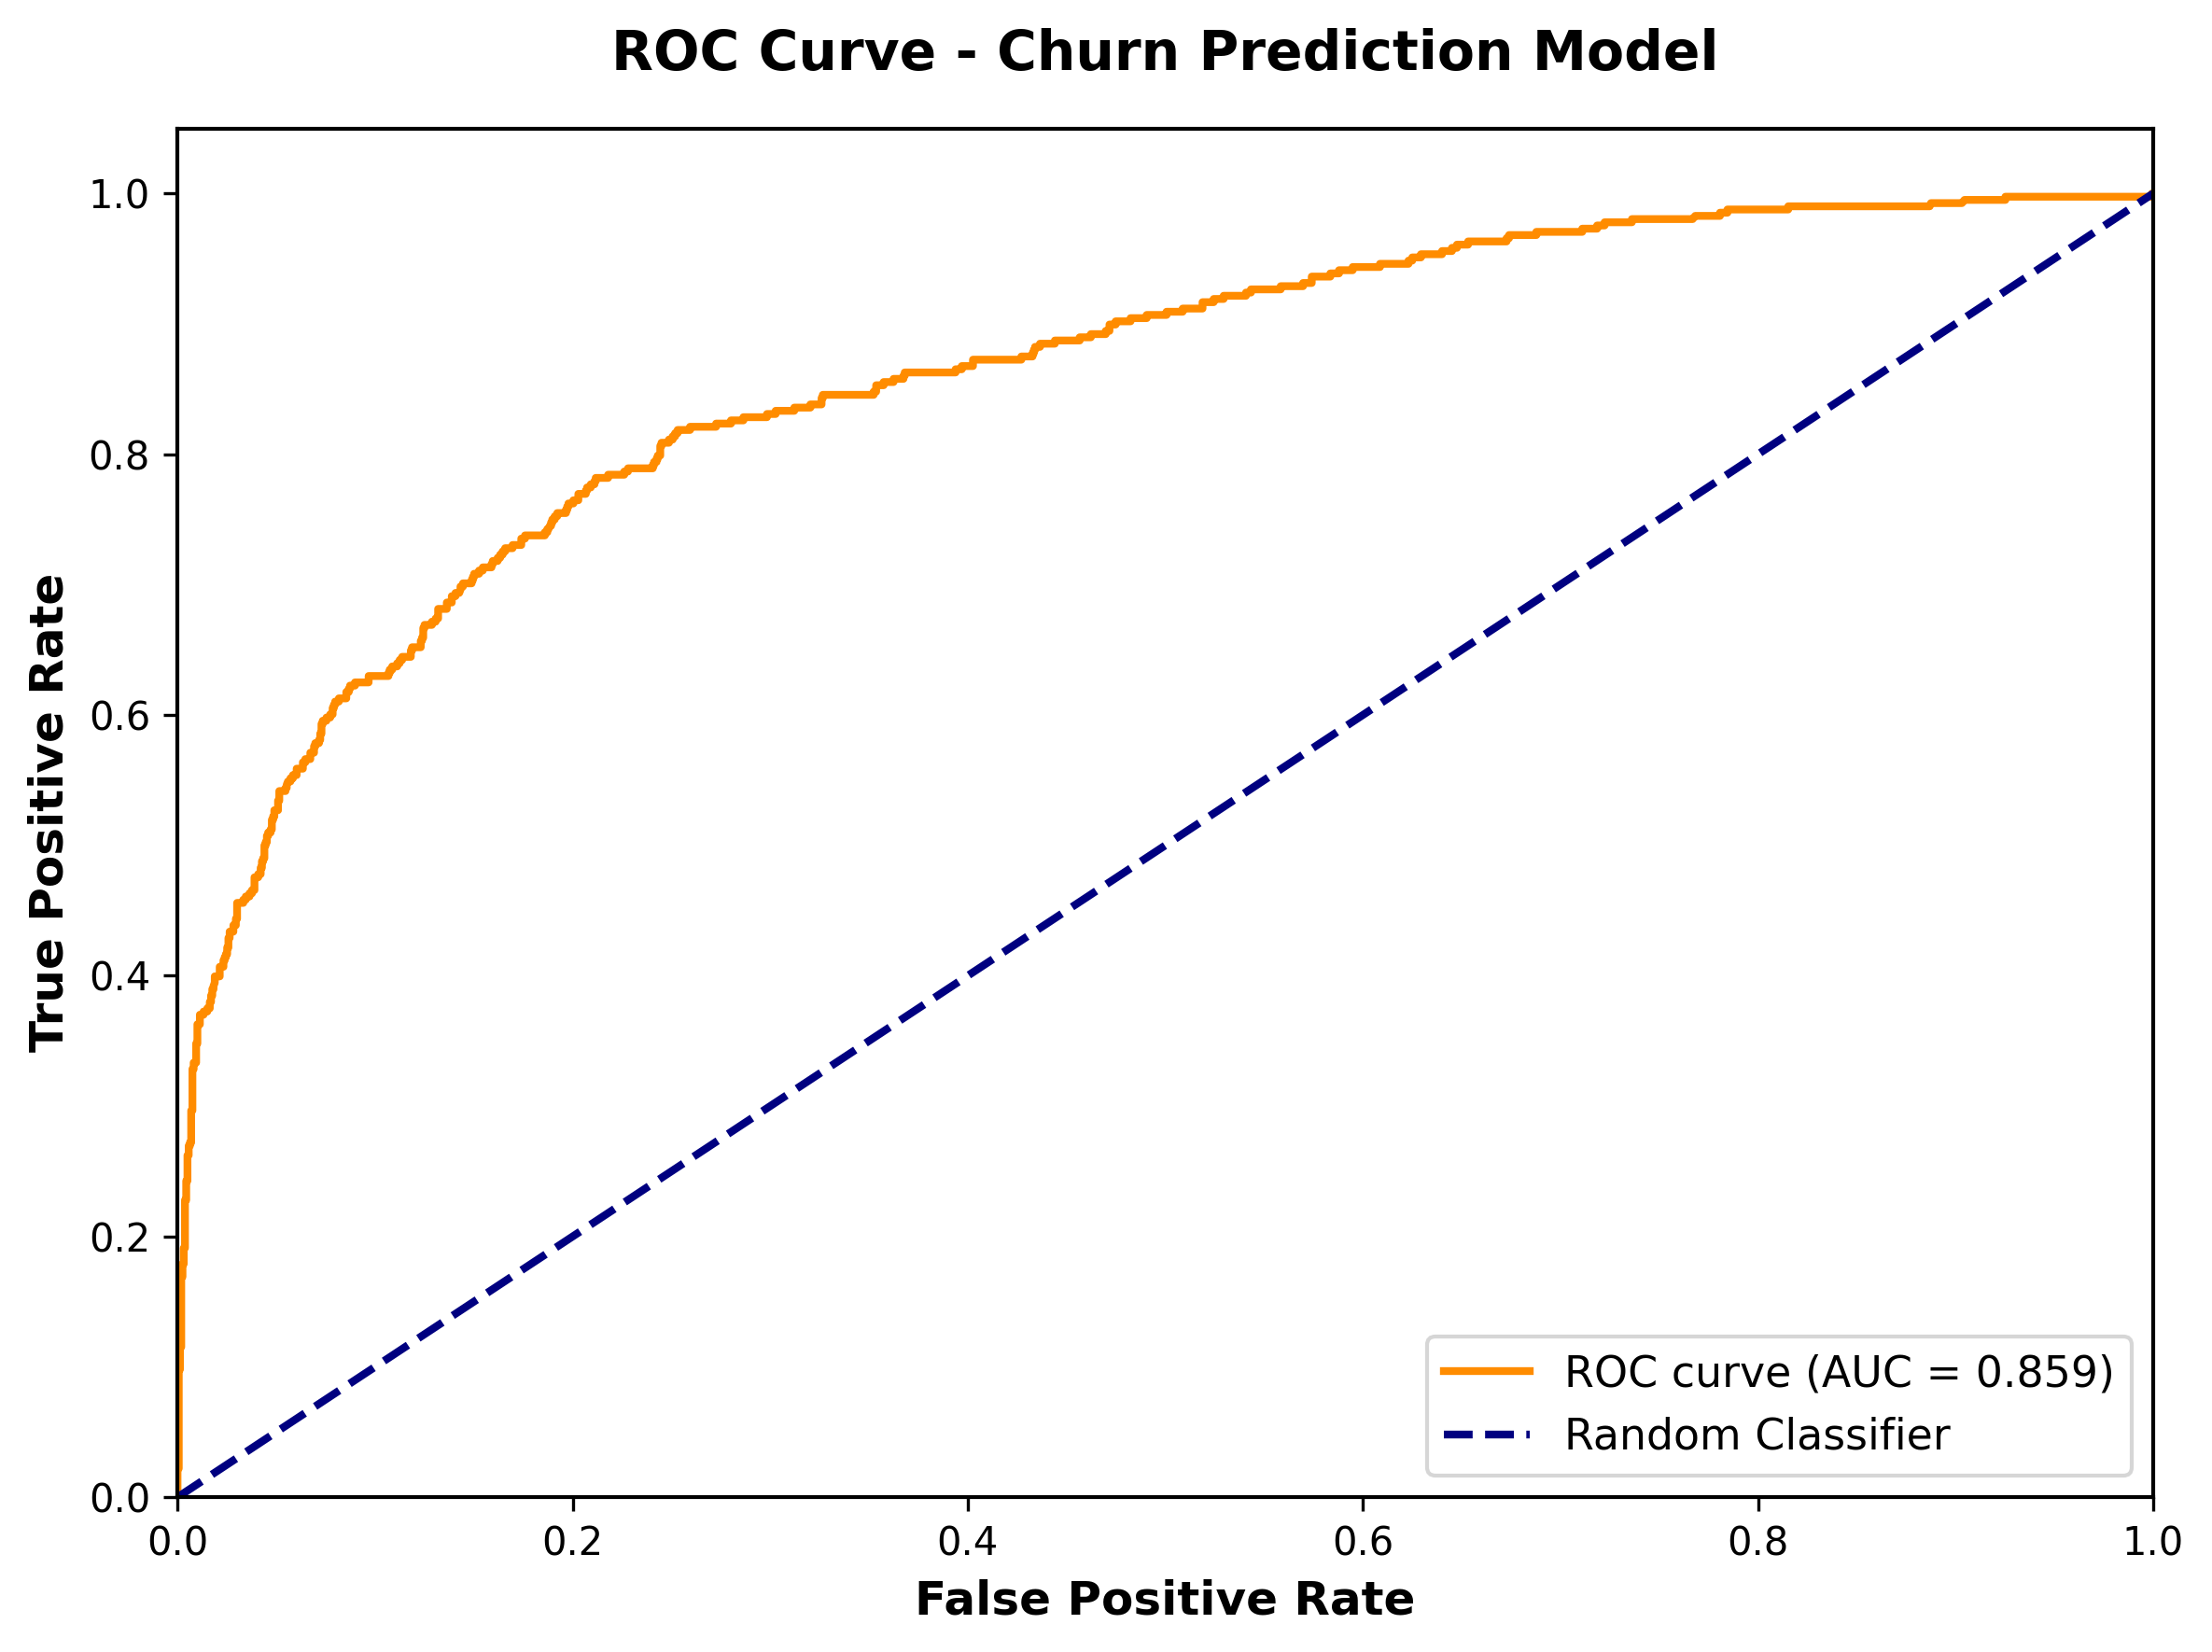
\includegraphics[width=0.7\textwidth]{img/17_roc_curve.png}
\caption{ROC curve showing strong discriminative power (AUC = 0.858)}
\label{fig:roc}
\end{figure}

\begin{figure}[H]
\centering
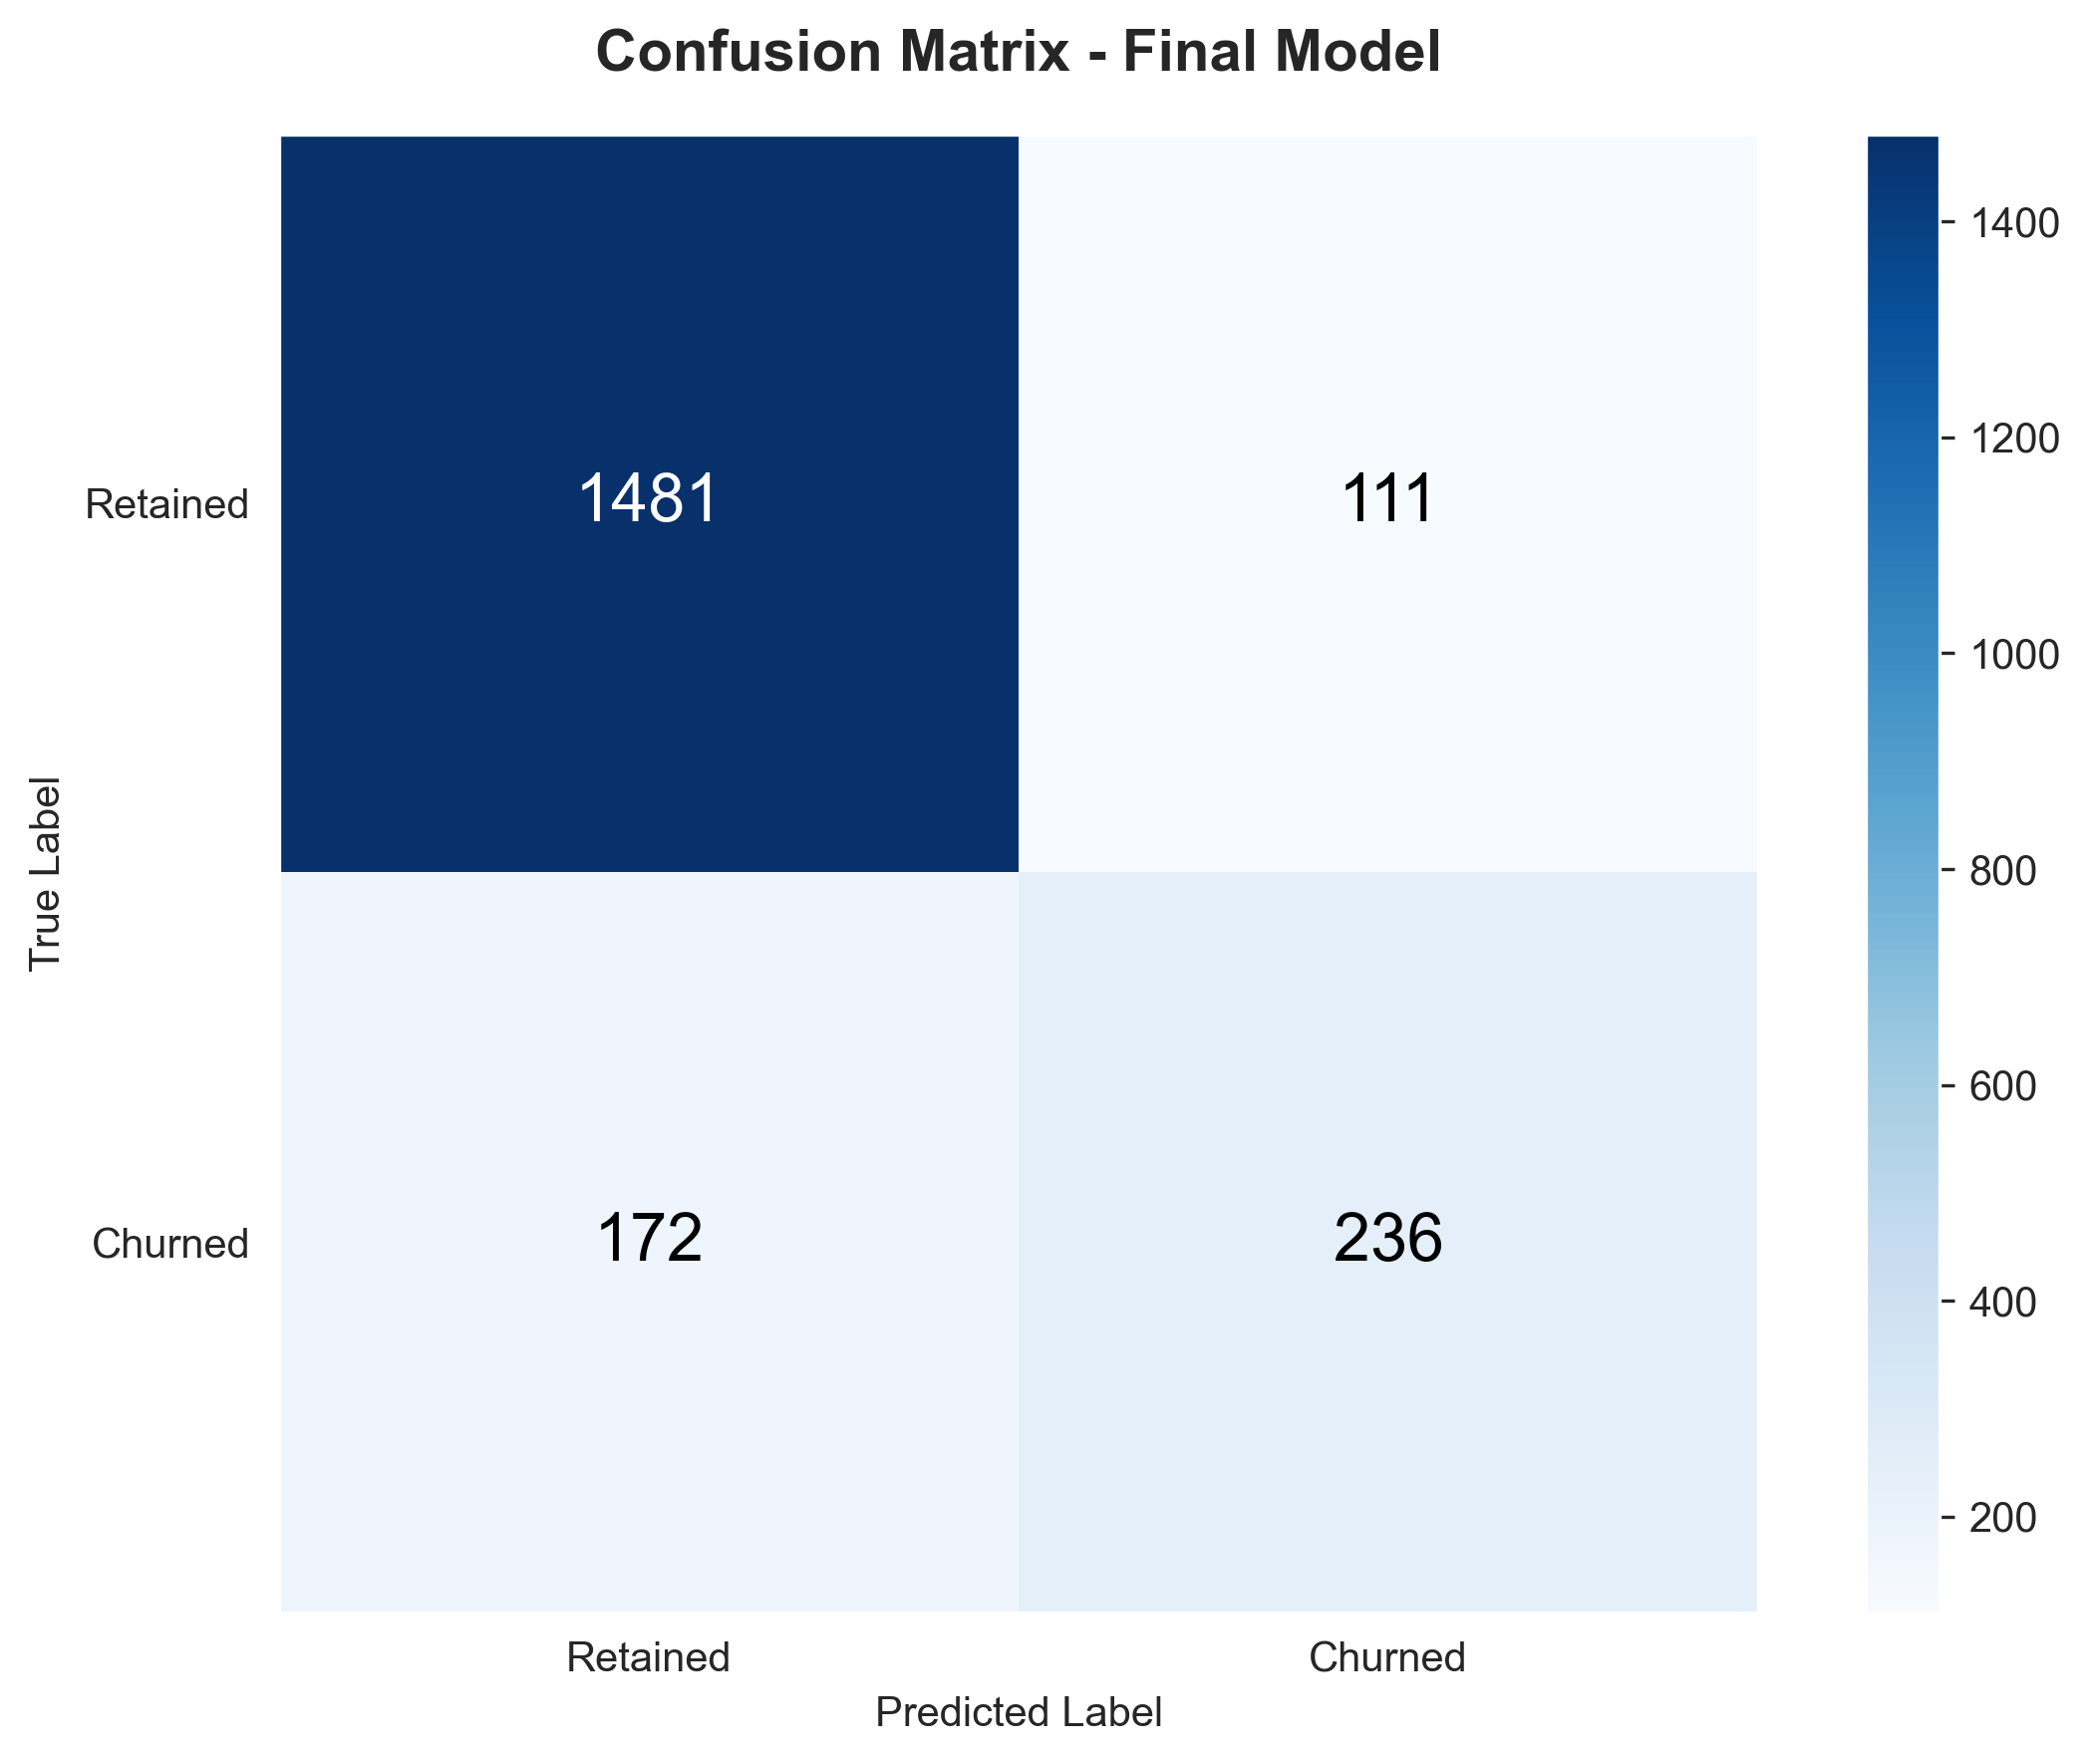
\includegraphics[width=0.6\textwidth]{img/16_confusion_matrix.png}
\caption{Confusion matrix showing model predictions vs actual churn}
\label{fig:confusion}
\end{figure}

Feature importance was assessed using built‑in impurity measures, permutation importance and SHAP (Shapley Additive Explanations) values (Figure~\ref{fig:feature_importance}).  Permutation importance measures the decrease in model performance when a feature is randomly shuffled:
\[ I_j = \mathbb{E}[L(y, f(\mathbf{x}_{\text{perm}(j)}))] - \mathbb{E}[L(y, f(\mathbf{x}))], \]
where \(\mathbf{x}_{\text{perm}(j)}\) denotes the feature vector with the \(j\)-th feature randomly permuted, and \(L\) is the loss function.  SHAP values provide a unified framework for feature attribution based on Shapley values from cooperative game theory.  For a model \(f\) and instance \(\mathbf{x}\), the SHAP value for feature \(j\) is
\[ \phi_j(f, \mathbf{x}) = \sum_{S \subseteq F \setminus \{j\}} \frac{|S|!(|F| - |S| - 1)!}{|F|!} [f(S \cup \{j\}) - f(S)], \]
where \(F\) is the set of all features, \(S\) is a subset of features, and \(f(S)\) is the model prediction using only features in \(S\).  Age and the number of products emerged as the most influential predictors: age contributed the largest SHAP impact on individual predictions, while the number of products showed the highest permutation importance.  Activity status, balance and German nationality were important but secondary drivers.  Partial dependence plots (Figures~\ref{fig:pdp_age} and~\ref{fig:pdp_products}) confirmed the U‑shaped effect of the number of products and the near‑monotonic increase in churn probability with age up to the 51–60 group.

\begin{figure}[H]
\centering
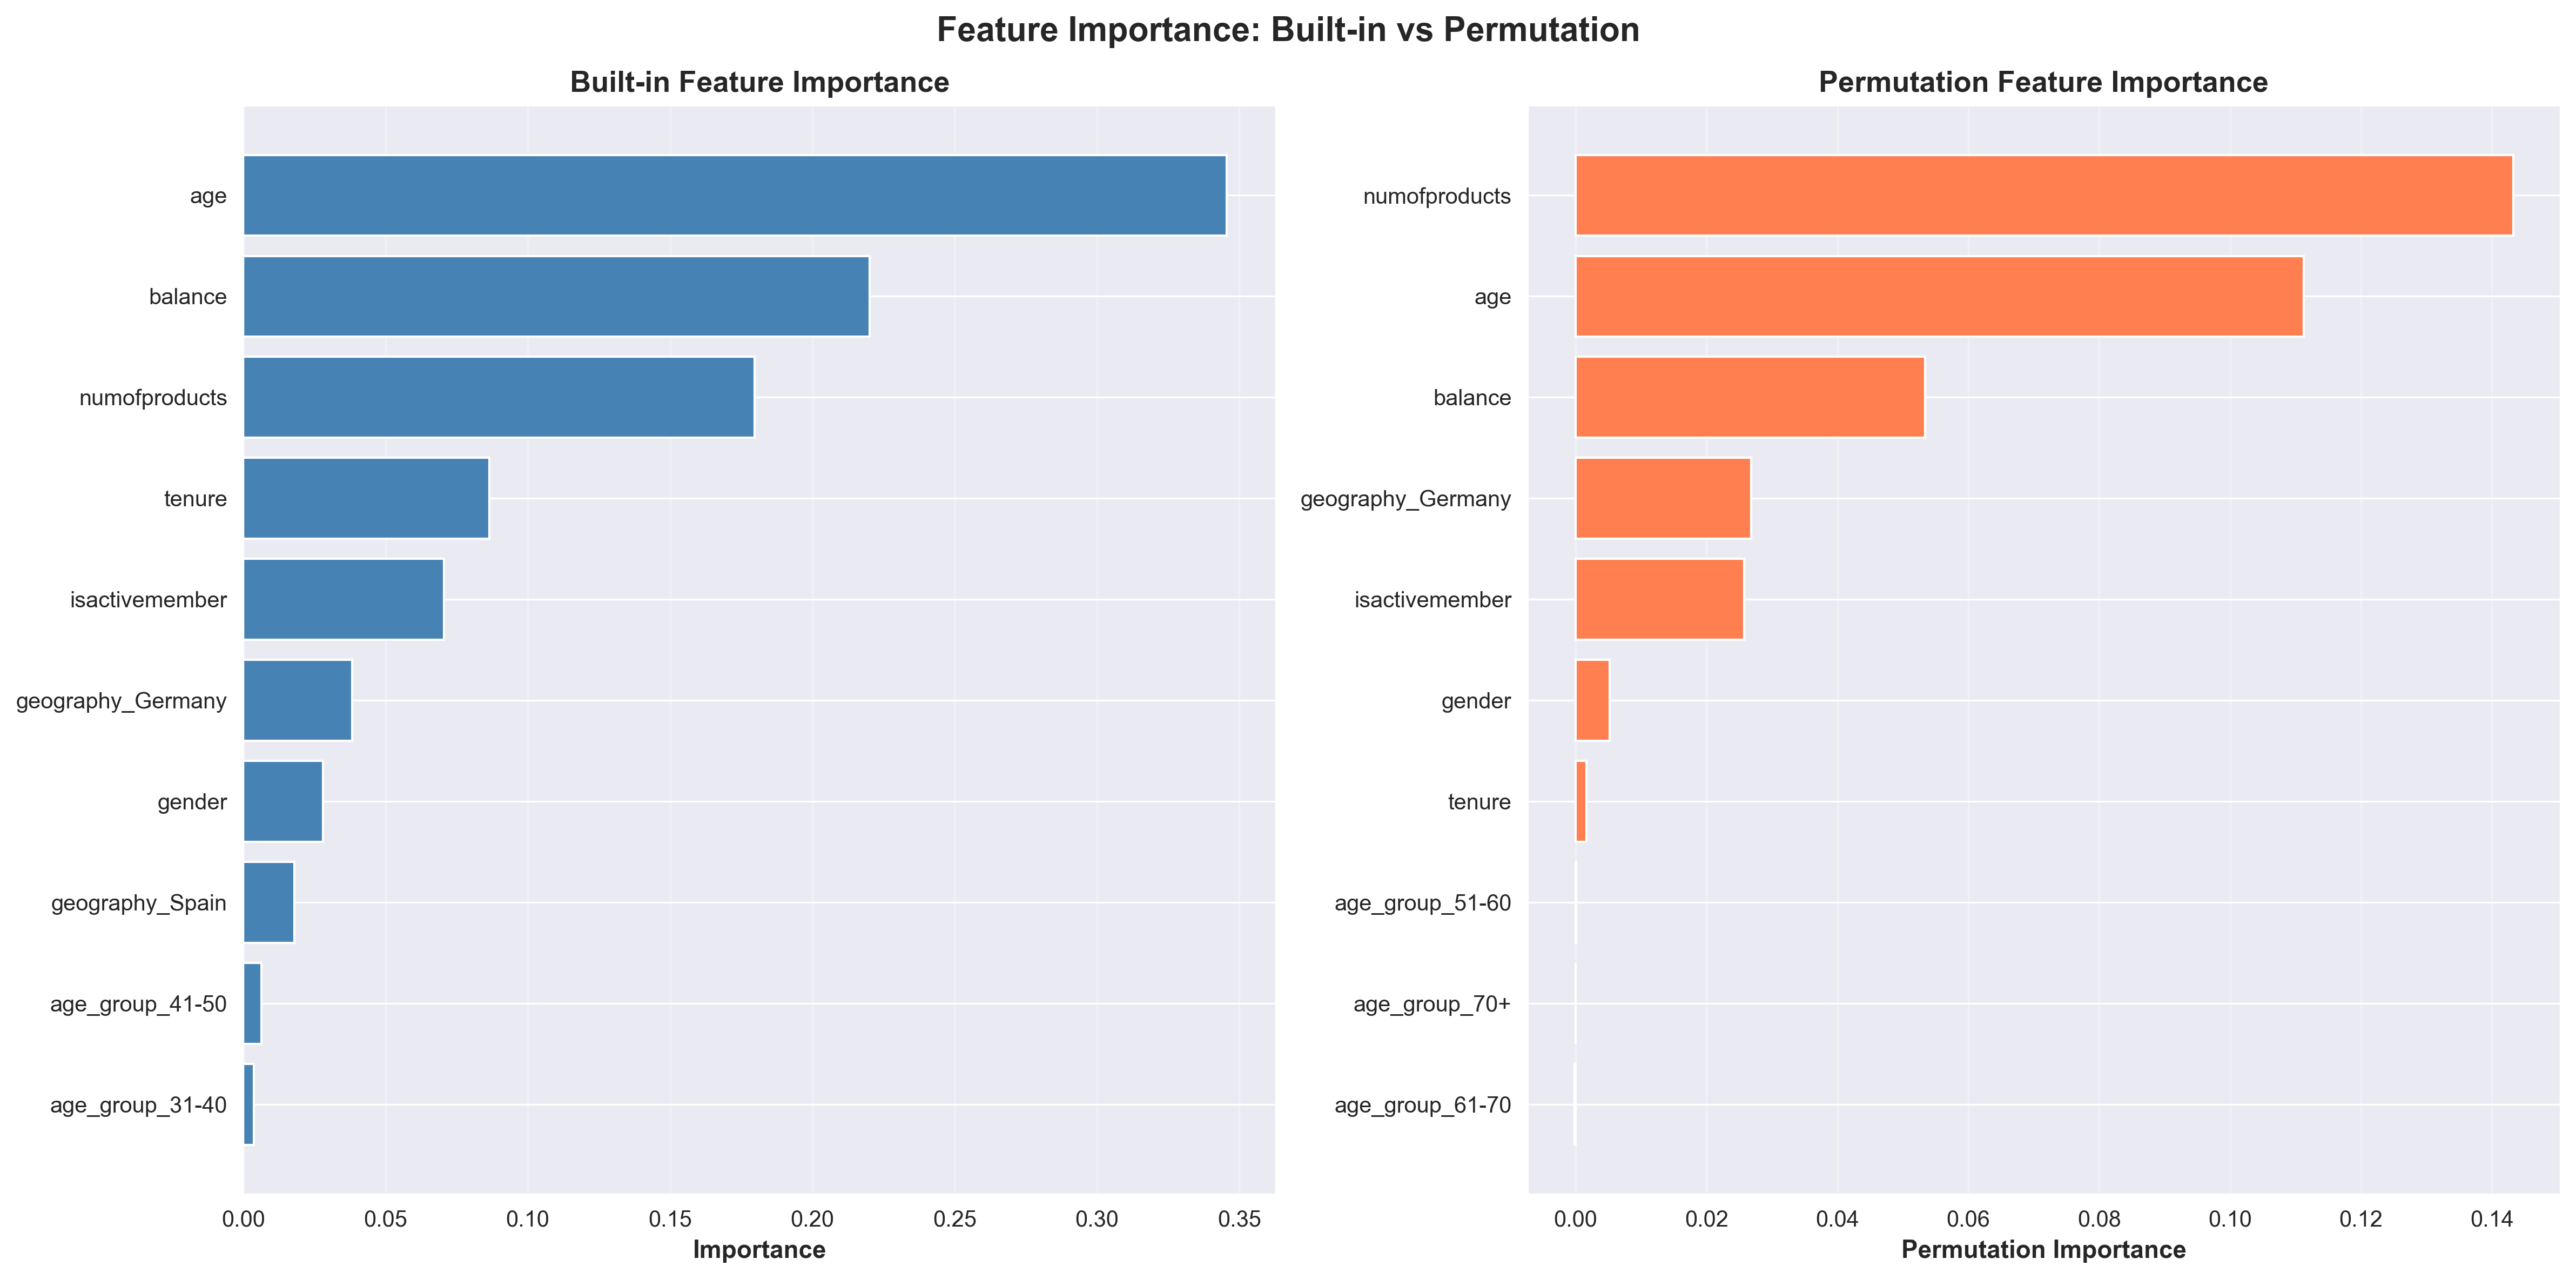
\includegraphics[width=0.8\textwidth]{img/15_feature_importance_comparison.png}
\caption{Feature importance comparison across three methods}
\label{fig:feature_importance}
\end{figure}

\begin{figure}[H]
\centering
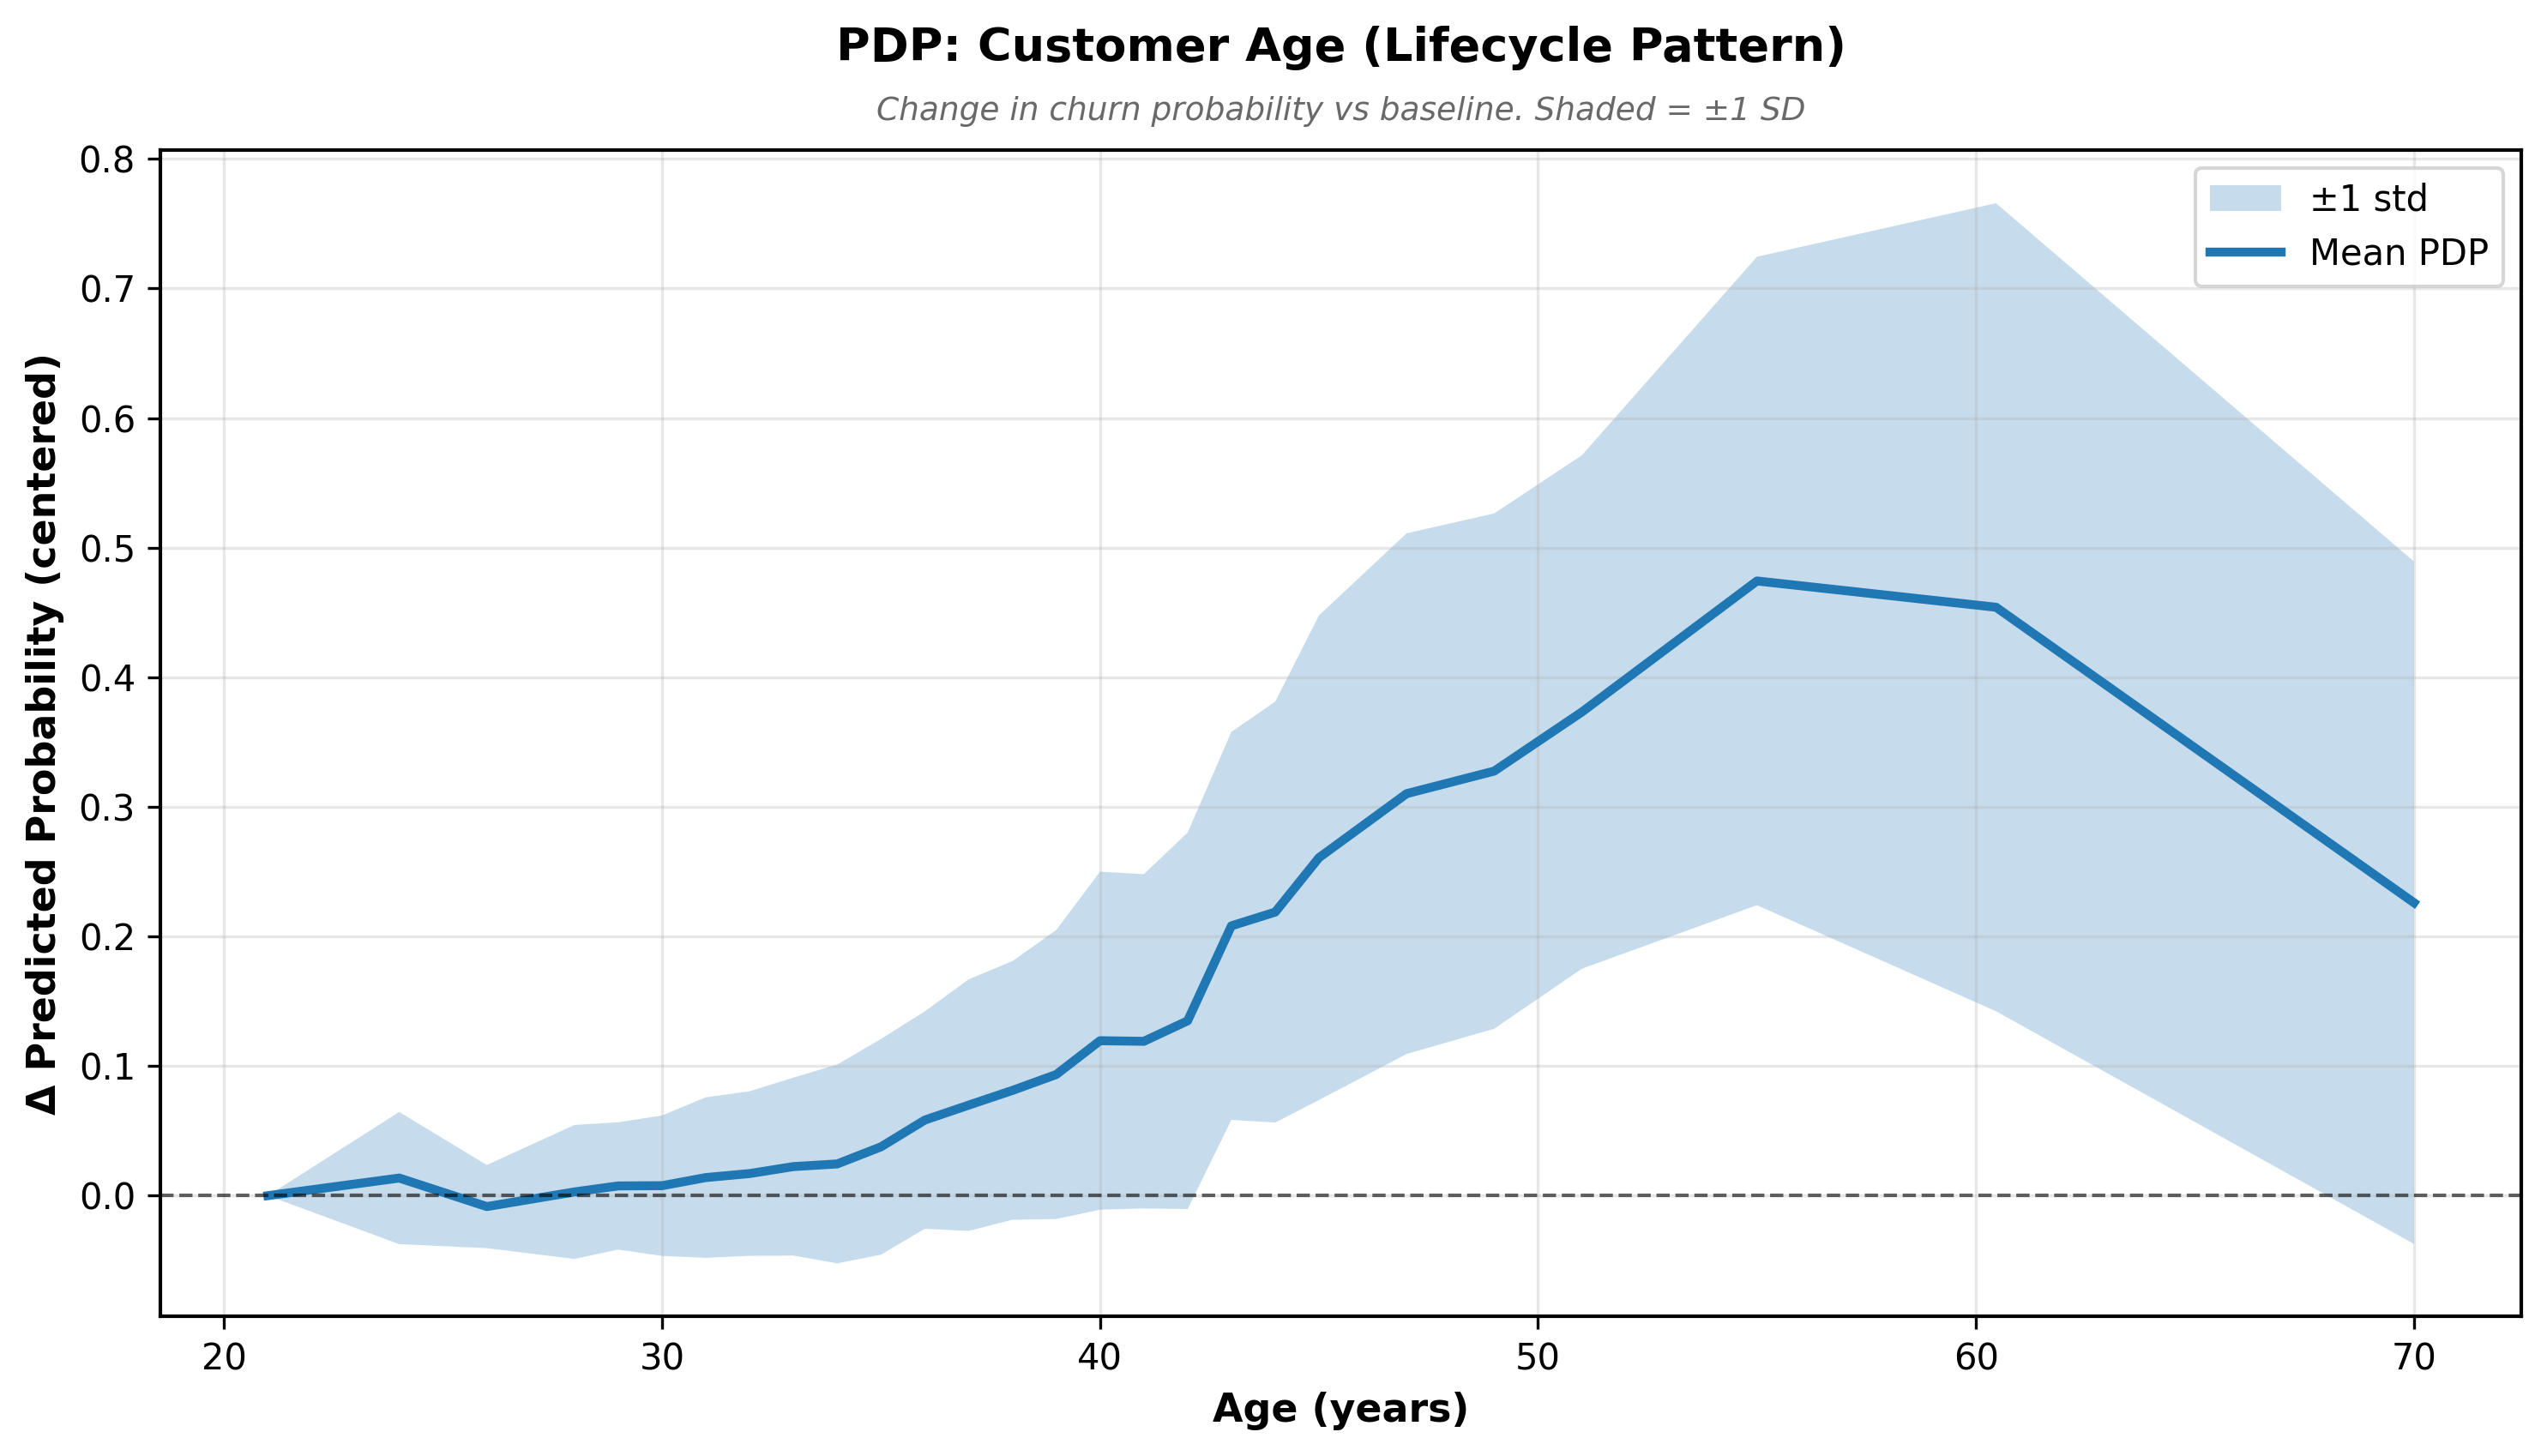
\includegraphics[width=0.6\textwidth]{img/18_pdp_age.png}
\caption{Partial dependence plot for age showing lifecycle churn pattern}
\label{fig:pdp_age}
\end{figure}

\begin{figure}[H]
\centering
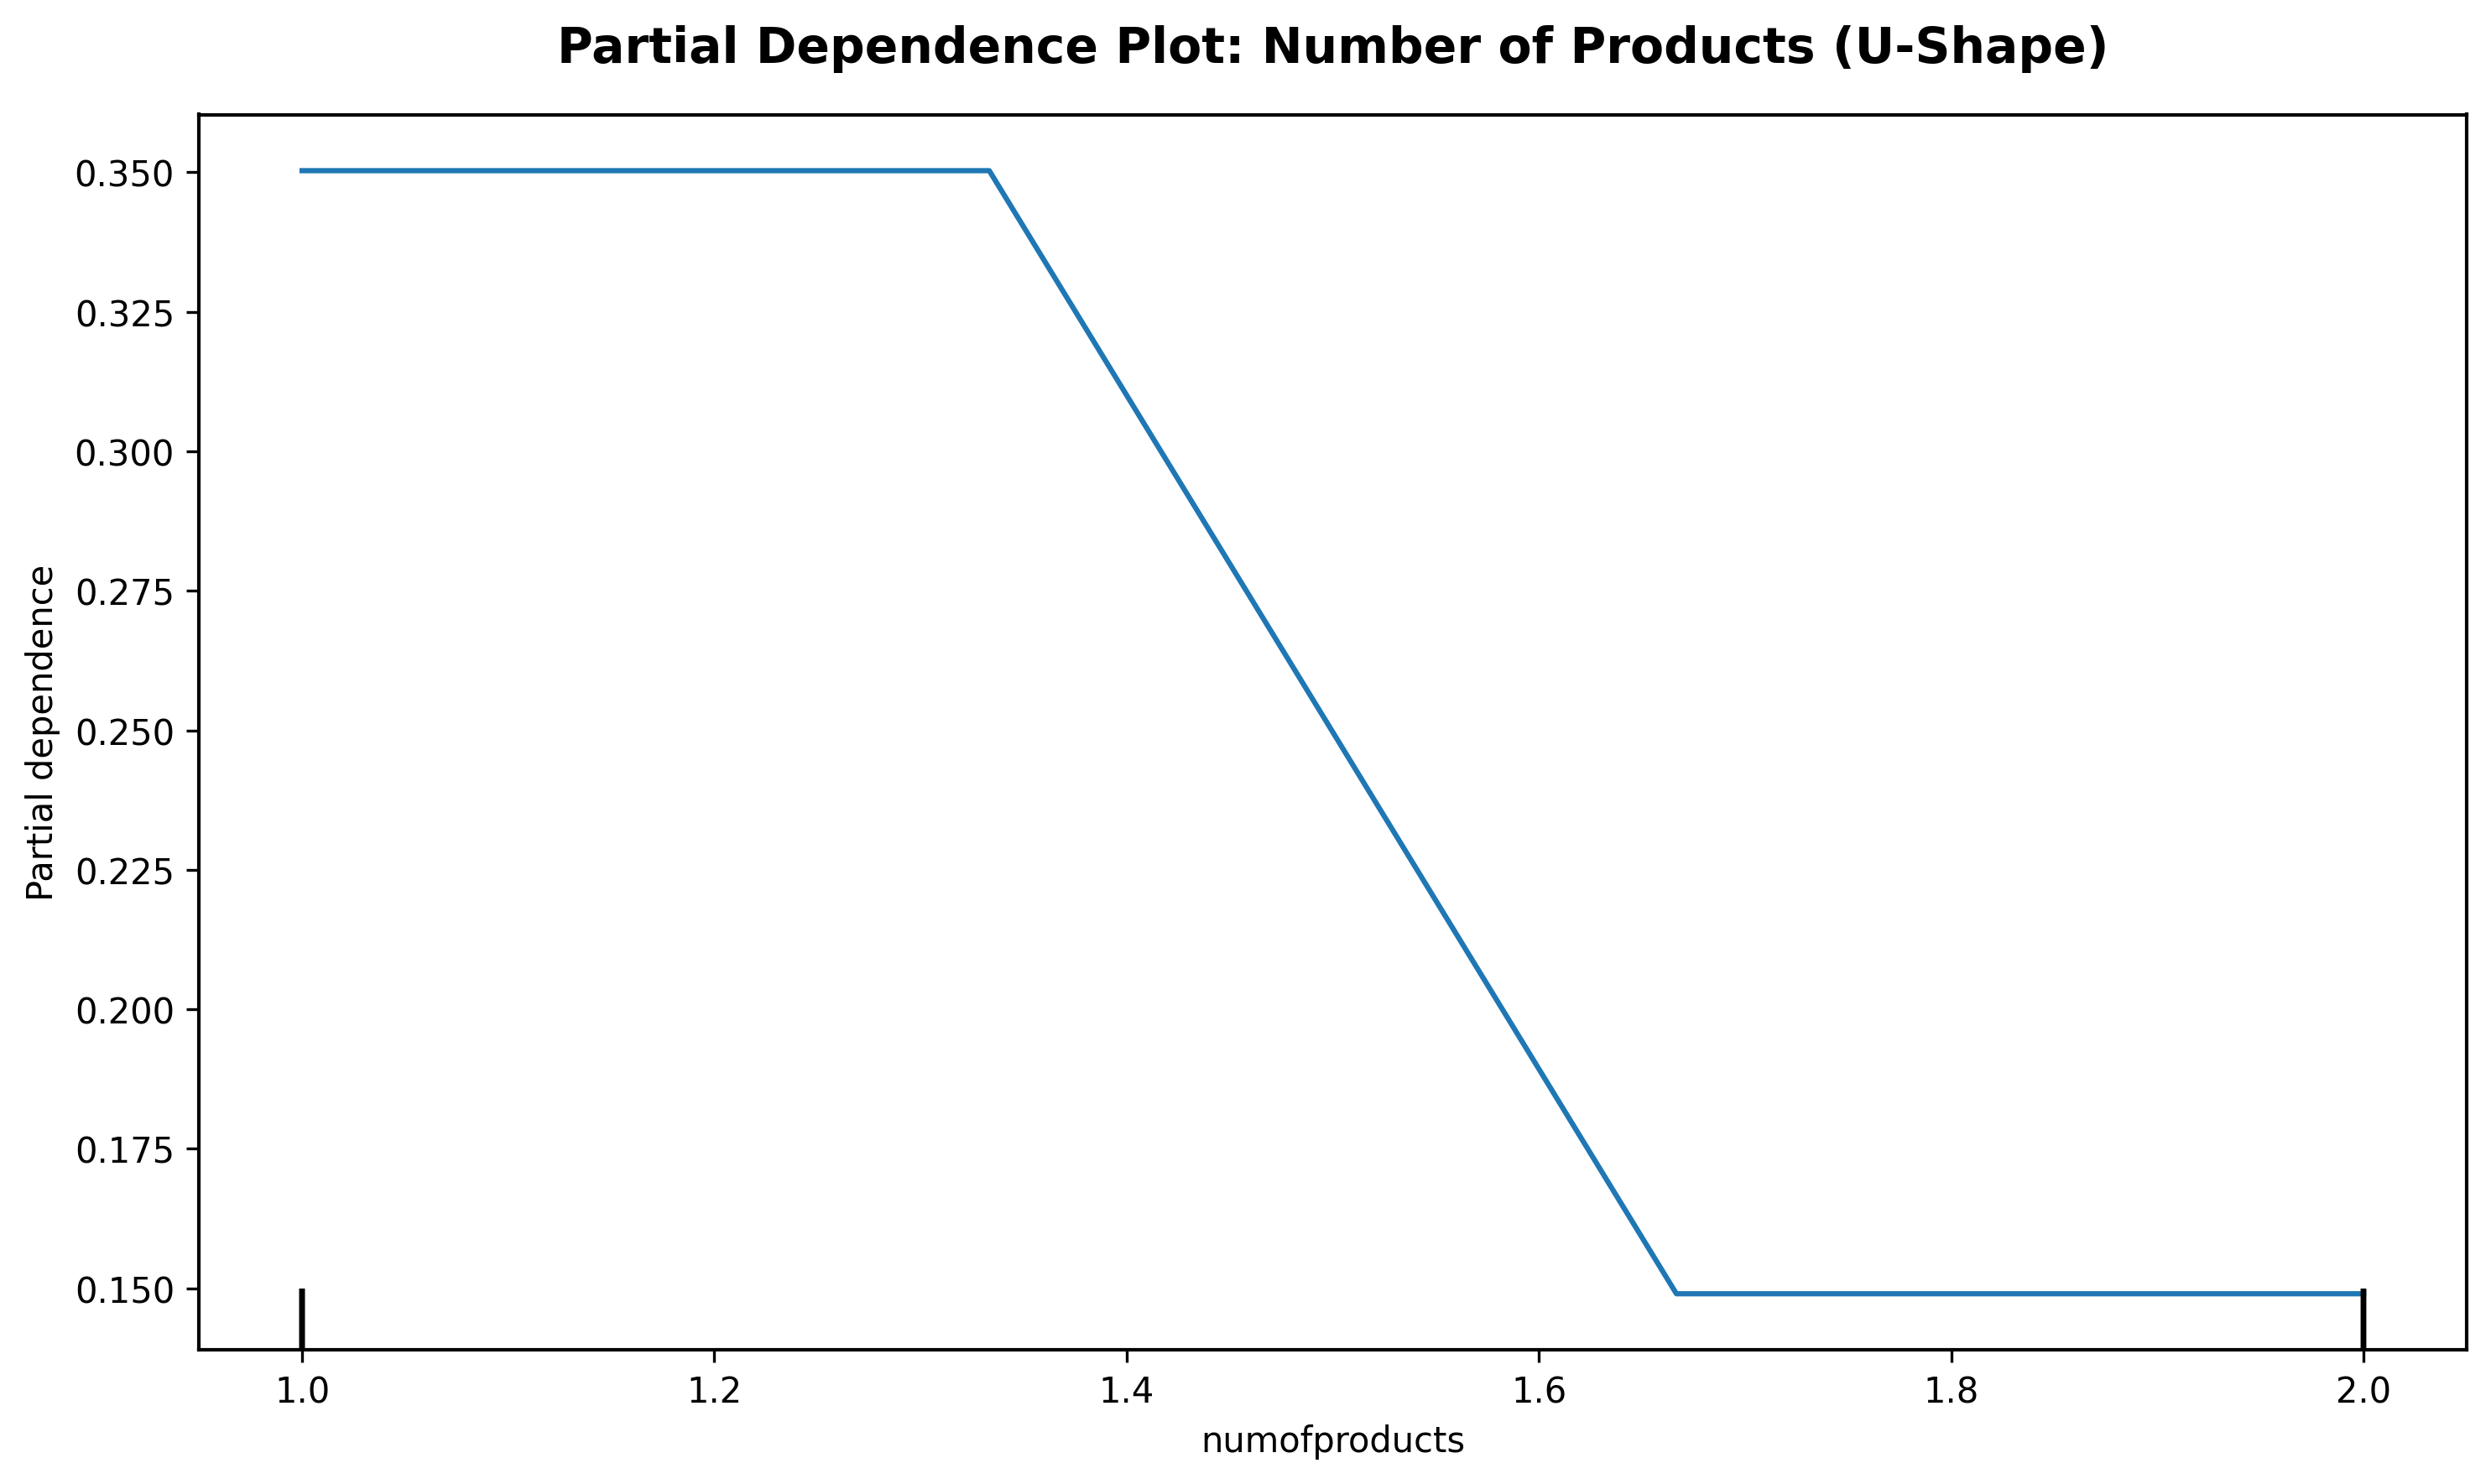
\includegraphics[width=0.6\textwidth]{img/19_pdp_numofproducts.png}
\caption{Partial dependence plot for number of products showing U‑shaped effect}
\label{fig:pdp_products}
\end{figure}

\begin{figure}[H]
\centering
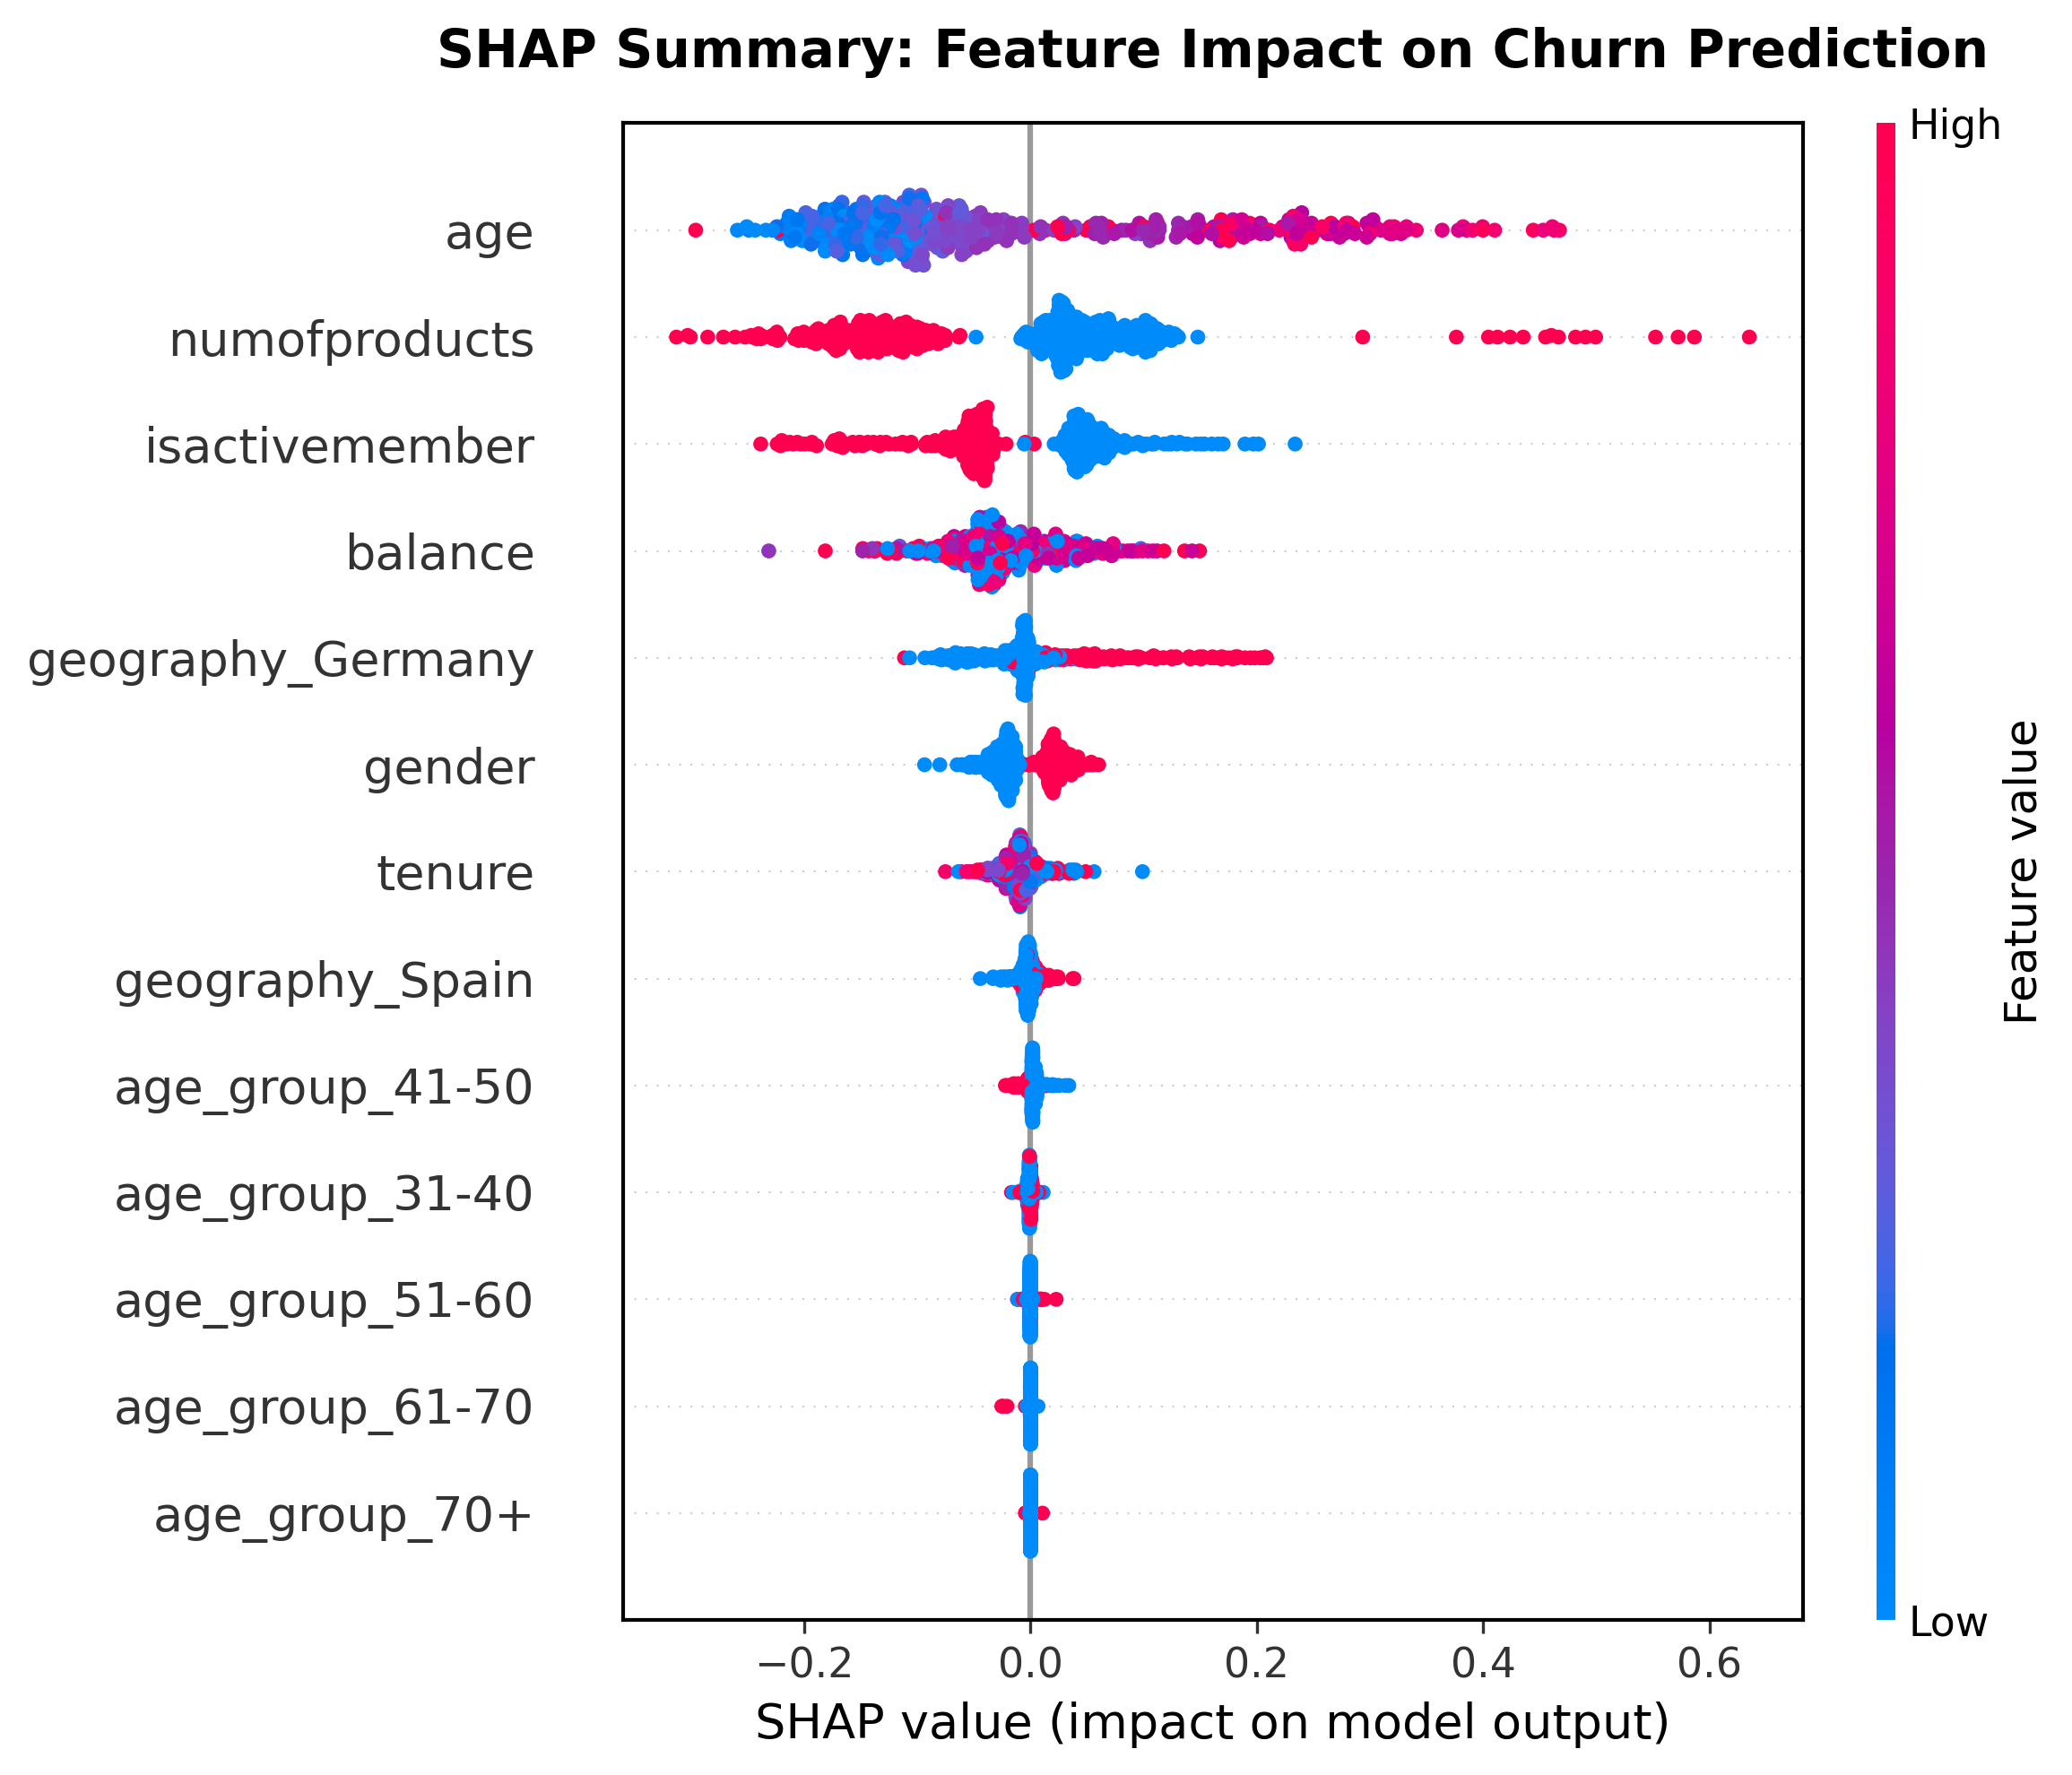
\includegraphics[width=0.7\textwidth]{img/20_shap_summary.png}
\caption{SHAP summary plot showing feature contributions to individual predictions}
\label{fig:shap}
\end{figure}

\subsection{Model Validation}
To ensure robustness, the random forest was compared against two gradient‑boosting alternatives: XGBoost and LightGBM (Figure~\ref{fig:model_comparison}).  All models were trained on identical splits and tuned with analogous hyperparameter searches.  Random forests slightly outperformed the alternatives in F1‑score (62.5~\% vs.\ 60.5–61.0~\%) and demonstrated more stable generalisation across folds.  A comprehensive metrics comparison (Figure~\ref{fig:metrics_comparison}) confirmed Random Forest's superiority.  Experiments evaluating synthetic minority oversampling (SMOTE) versus class weighting (Figure~\ref{fig:smote_roc}) revealed that SMOTE increased recall at the expense of a substantial rise in false positives; class weights offered a more balanced trade‑off.  Additional engineered features (interaction terms and polynomial expansions) did not improve performance, underscoring that tree‑based methods inherently capture non‑linear interactions.

\begin{figure}[H]
\centering
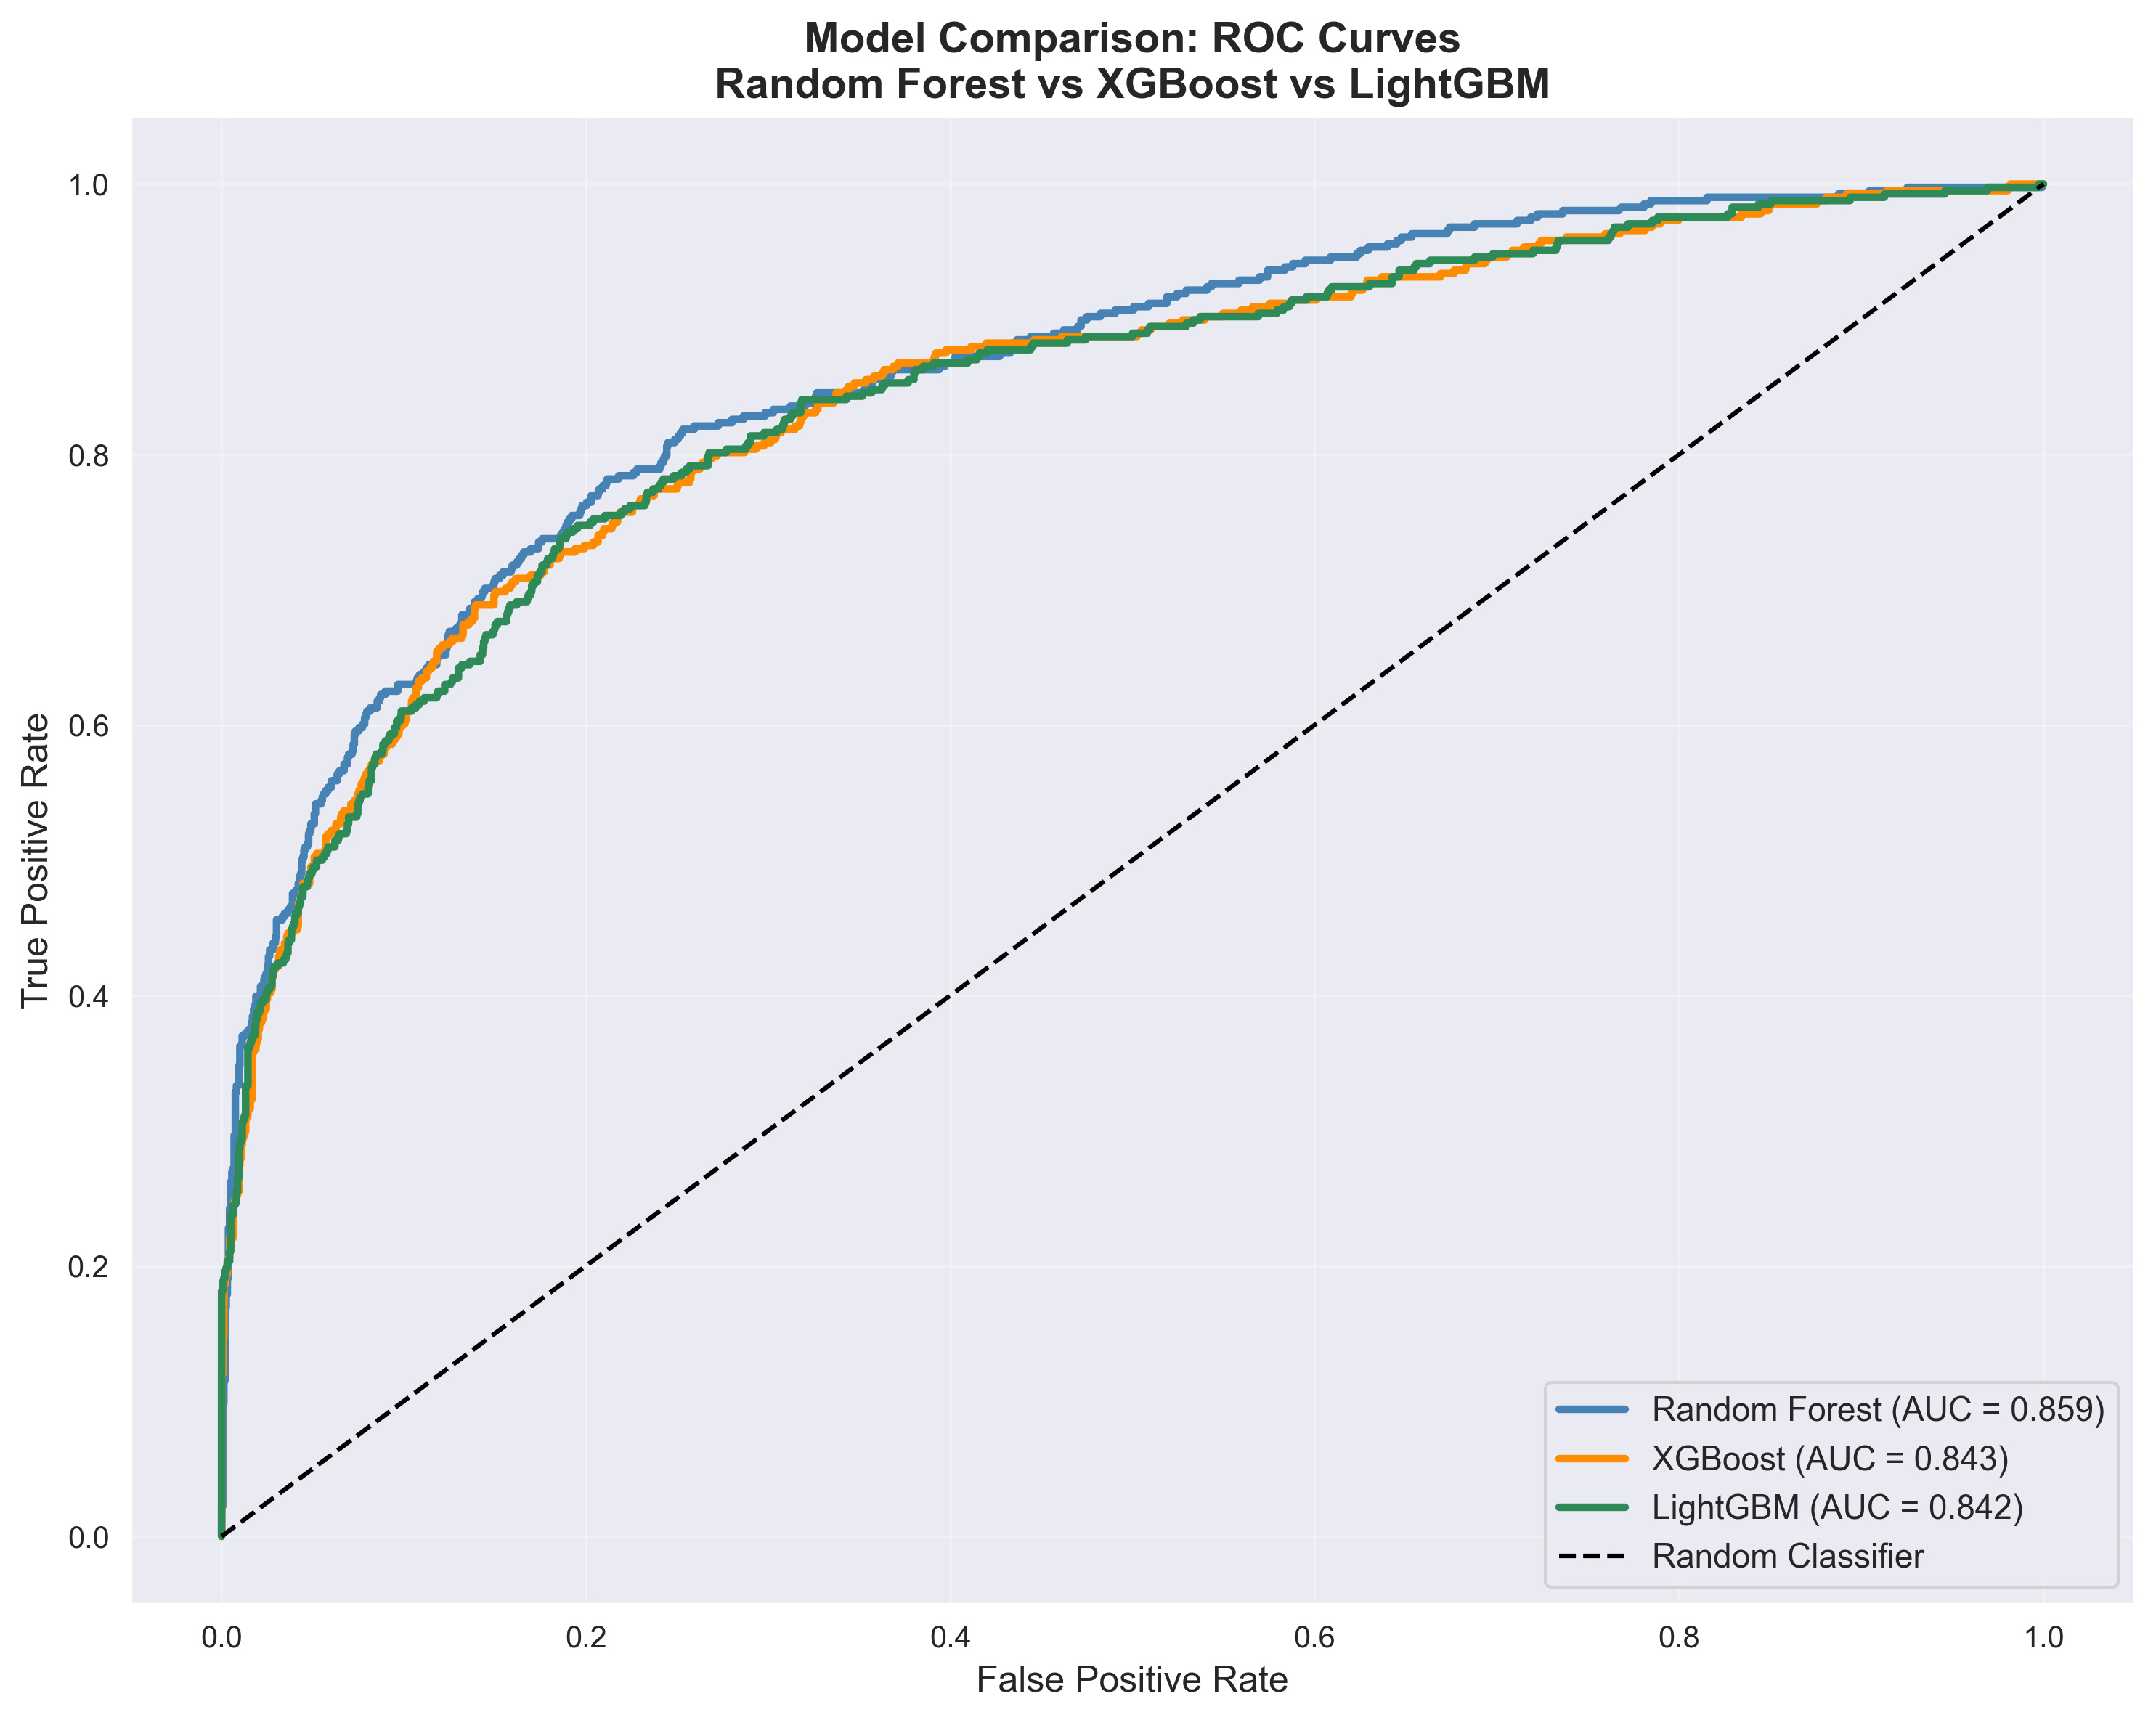
\includegraphics[width=0.7\textwidth]{img/21_model_comparison_roc.png}
\caption{ROC curve comparison: Random Forest vs XGBoost vs LightGBM}
\label{fig:model_comparison}
\end{figure}

\begin{figure}[H]
\centering
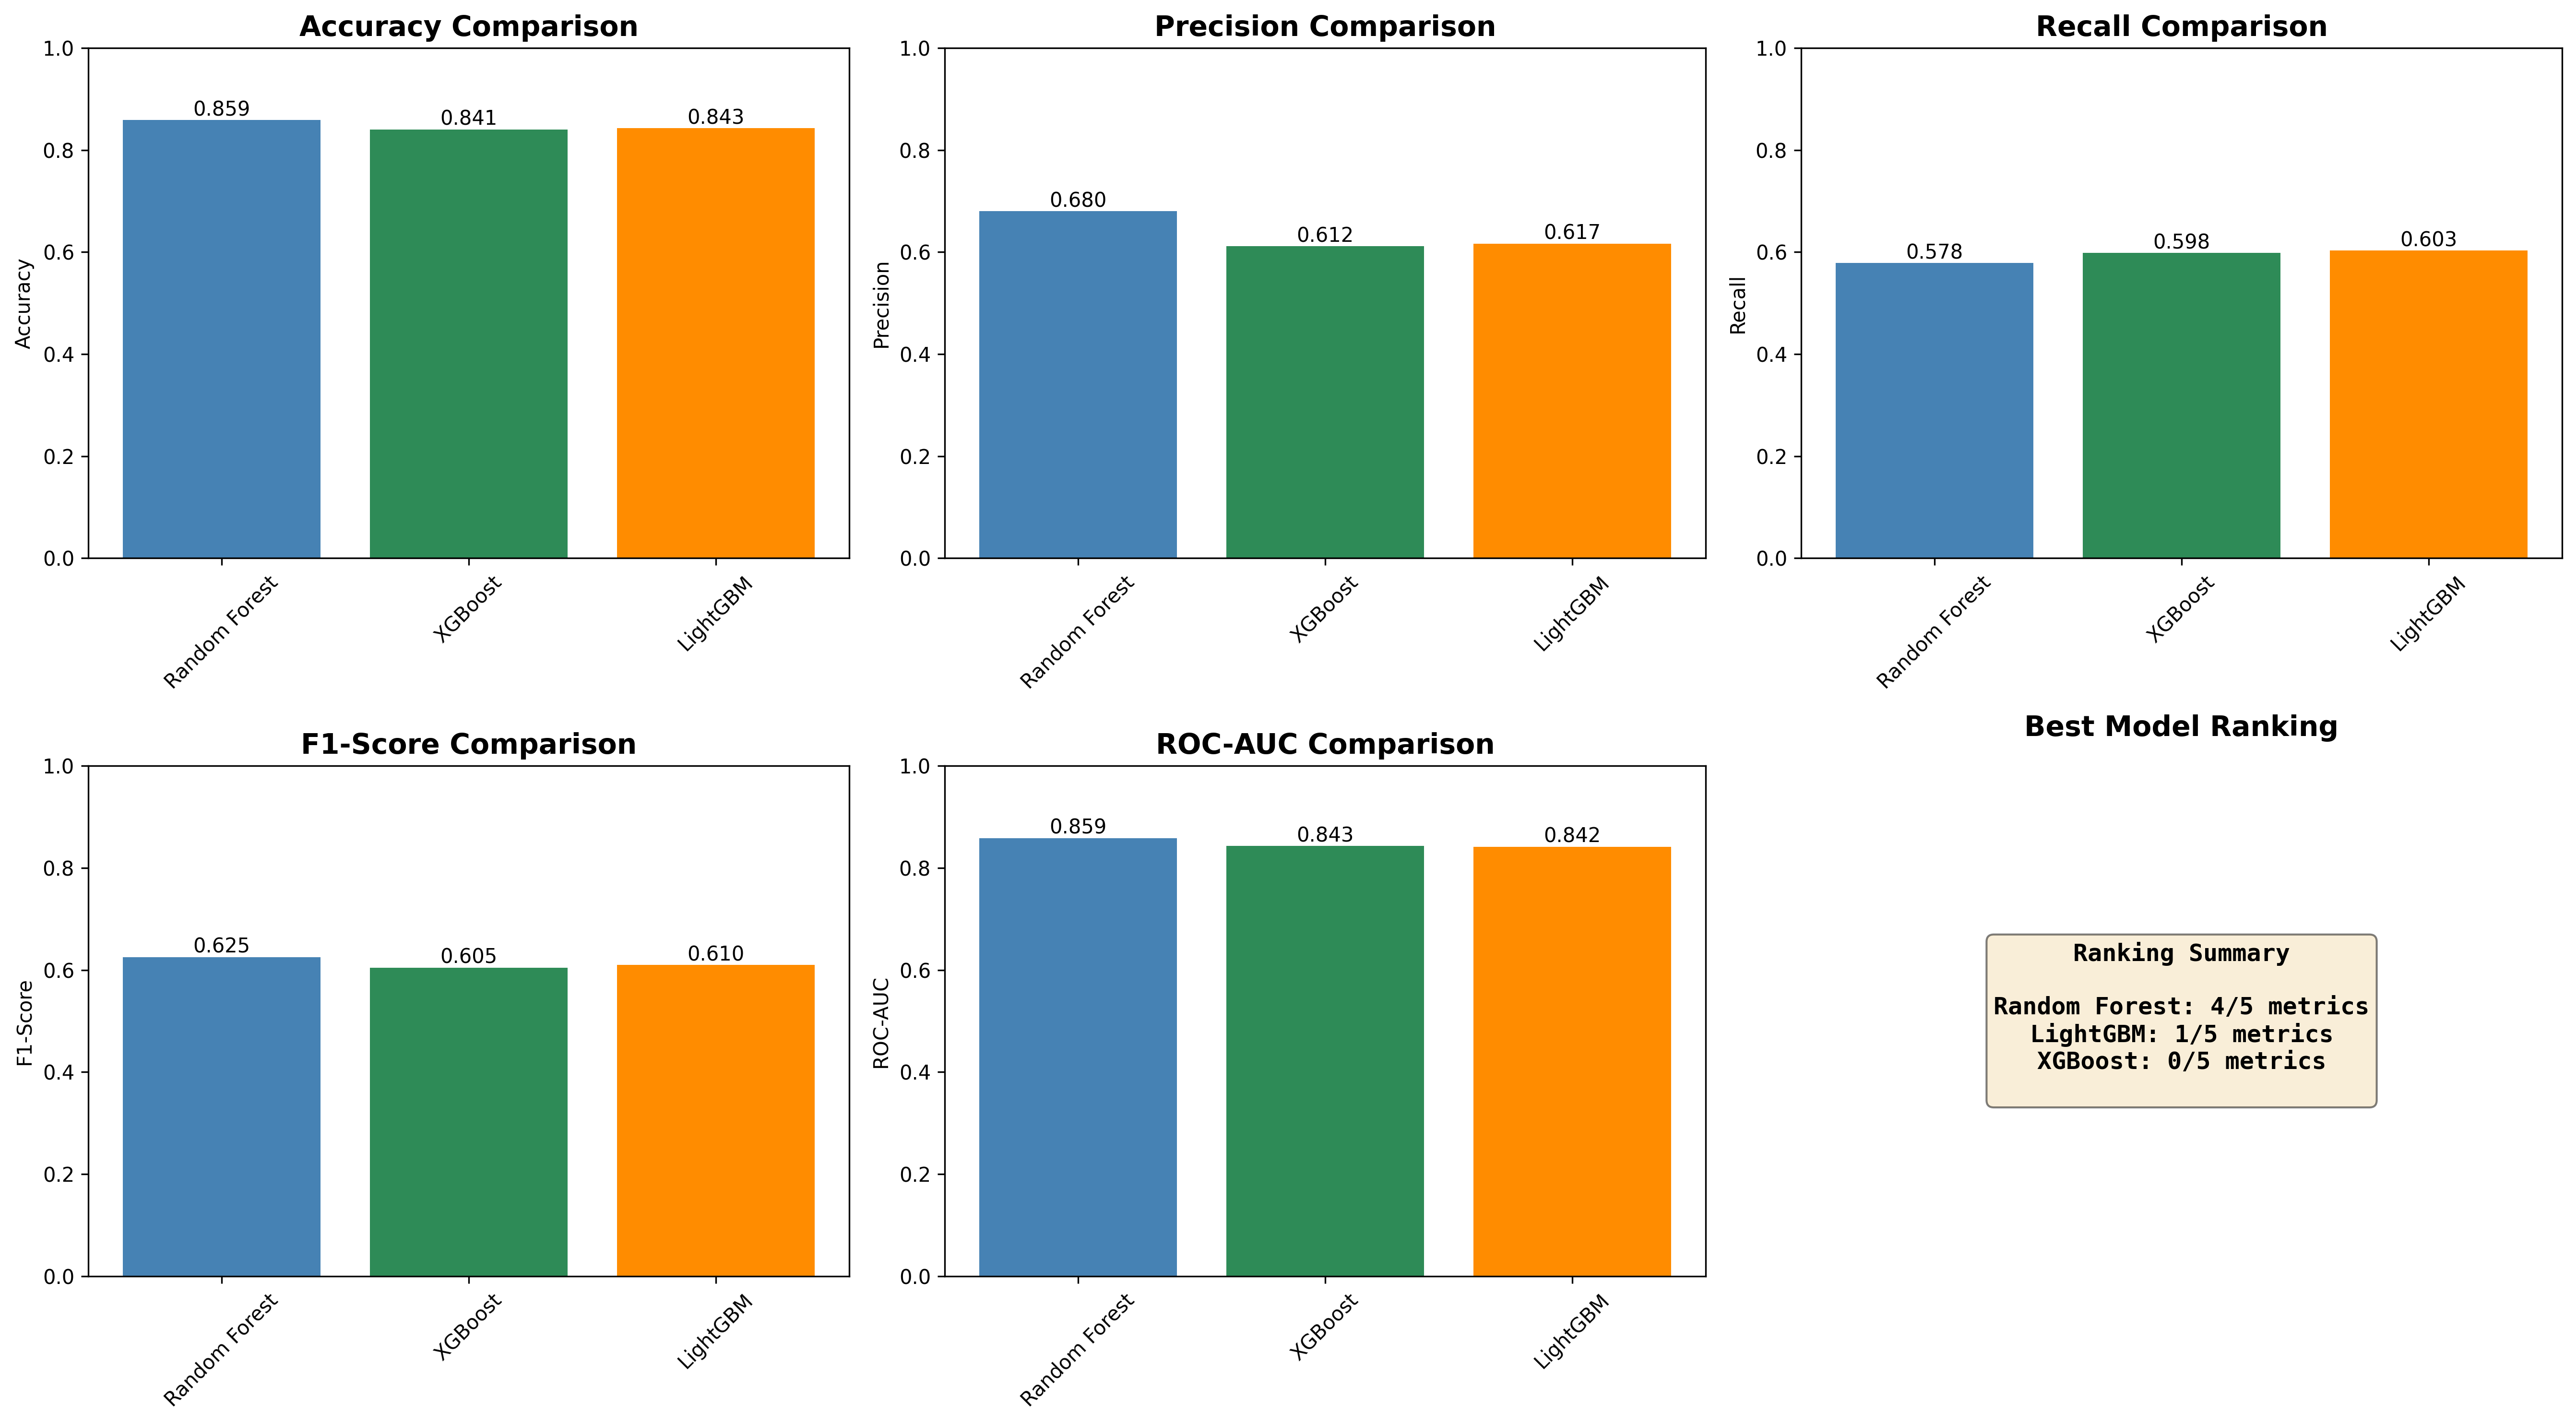
\includegraphics[width=0.9\textwidth]{img/24_model_comparison_metrics.png}
\caption{Comprehensive metrics comparison across three algorithms}
\label{fig:metrics_comparison}
\end{figure}

\begin{figure}[H]
\centering
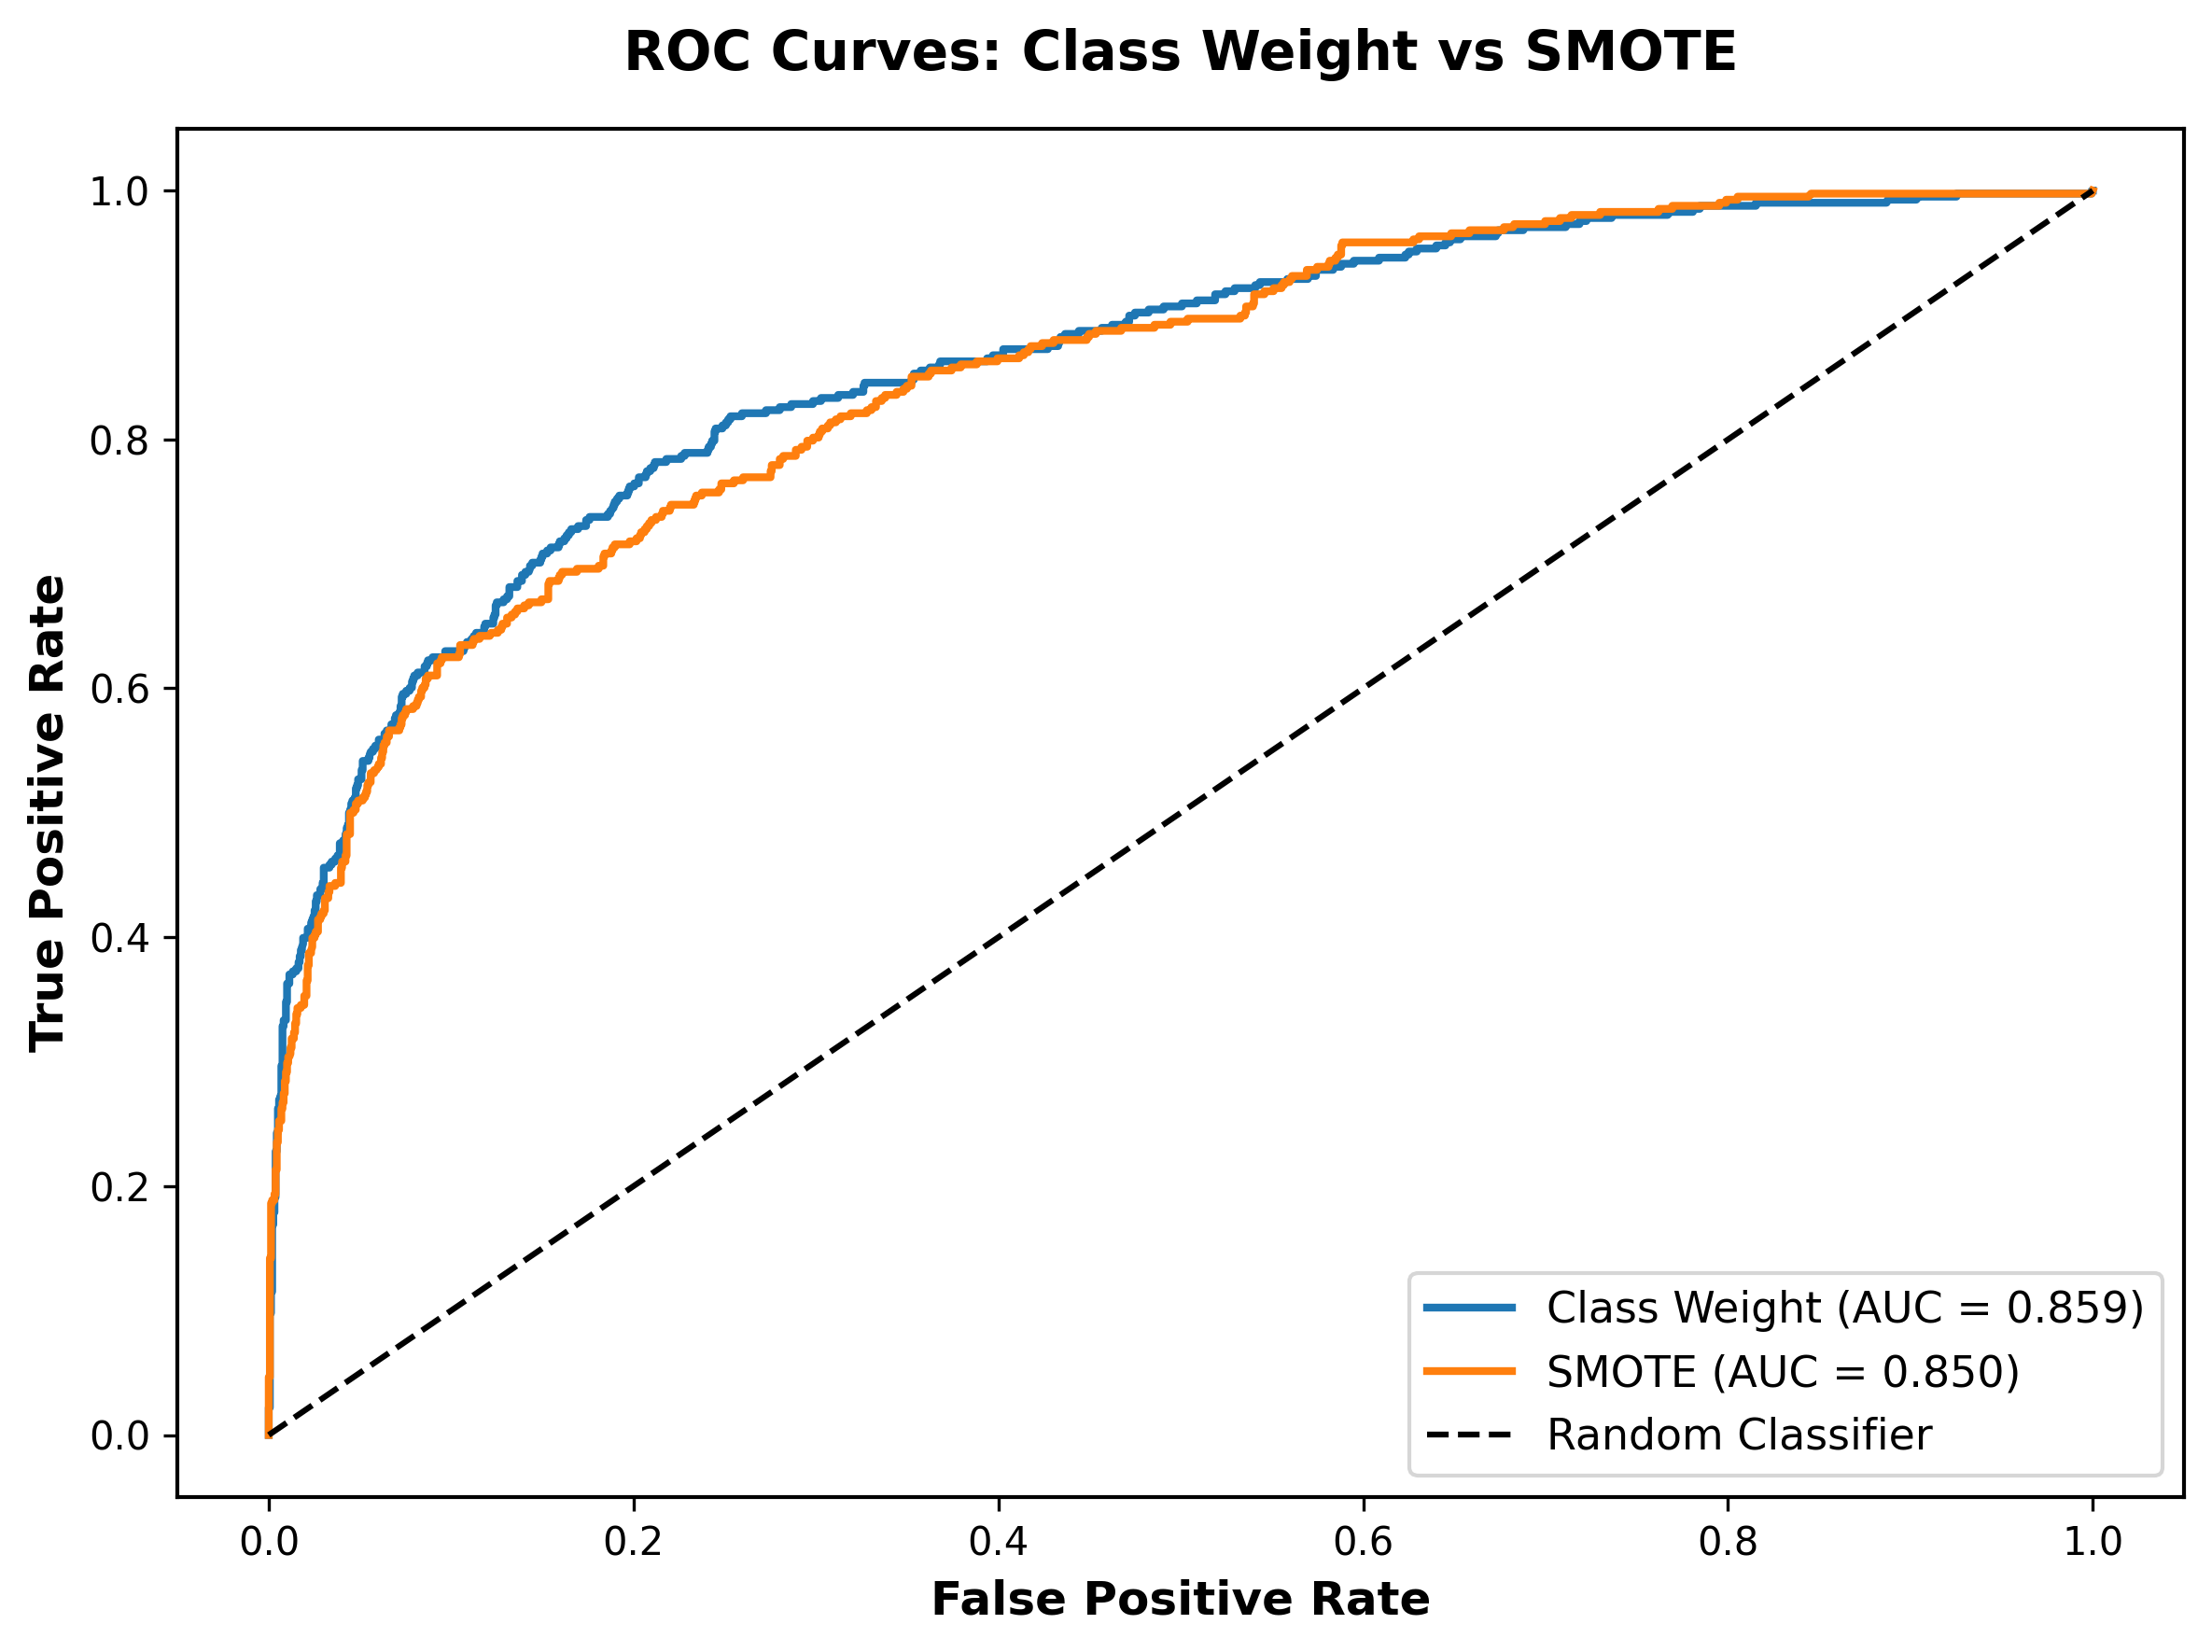
\includegraphics[width=0.7\textwidth]{img/25_smote_roc_comparison.png}
\caption{SMOTE vs class weight ROC comparison}
\label{fig:smote_roc}
\end{figure}

\section{Discussion}
\subsection{Key Findings}
The combined analyses yielded several actionable insights:

\begin{enumerate}
  \item \textbf{Complaint status is a lagging indicator of churn.}  Virtually every customer who filed a complaint subsequently exited.  While this makes complaint status a perfect predictor, it is unsuitable for proactive intervention because it signals churn after dissatisfaction has reached an irreparable level.  Complaint prevention, therefore, is critical and should be addressed separately.

  \item \textbf{Product portfolio has a Goldilocks zone.}  Customers with two products displayed the lowest churn, whereas those with three or four products experienced extremely high attrition.  The dramatic U‑shaped relationship suggests that cross‑selling beyond two products backfires.  Targeted portfolio capping at two products and consolidation of over‑sold customers could save hundreds of accounts annually.

  \item \textbf{Lifecycle stage drives churn risk.}  Age exhibited a strong non‑linear effect, with the 51–60 cohort showing a hazard ratio of 7.94 relative to the youngest group.  This demographic corresponds to pre‑retirement customers who may consolidate assets or seek better retirement products elsewhere.  Specialised retention programmes focusing on retirement planning and personalised services are warranted.

  \item \textbf{Engagement is the strongest modifiable predictor.}  Active membership is associated with a 46~\% reduction in churn hazard.  Re‑engagement campaigns targeting inactive customers (through personalised communications, gamification and incentives) represent a promising lever for retention.

  \item \textbf{Geography matters.}  German customers exhibited twice the churn rate of French and Spanish customers and a hazard ratio of 1.60.  Market‑specific issues such as competition, regulation or service quality likely underlie this disparity and require targeted investigation and localisation strategies.
\end{enumerate}

These findings are supported by both the survival model and the random forest classifier, reinforcing the validity of the patterns.  Importantly, the risk factors vary in modifiability: age and geography are inherent, whereas number of products and activity status are under managerial control.  Effective retention strategies should therefore prioritise modifiable drivers.

\subsection{Methodological Considerations and Model Interpretation}
It is worth contextualising the model's performance metrics (85.9~\% accuracy, 68.0~\% precision, 57.8~\% recall) relative to other analyses of this dataset.  Many published analyses achieve near‑perfect accuracy by including complaint status as a predictive feature, as it exhibits an almost perfect correlation with churn (\(r=0.996\)).  While such models may appear impressive on paper, they represent a fundamental misunderstanding of the predictive modeling task: complaint status is a lagging indicator that signals churn has already occurred or is imminent, rendering it useless for proactive intervention.

The decision to exclude complaint status sacrifices headline accuracy metrics for genuine predictive utility.  A model that relies heavily on complaint status may achieve 99~\% accuracy, but it identifies customers who have already expressed dissatisfaction through formal channels—exactly when retention is least likely to succeed.  In contrast, the present model achieves 85.9~\% accuracy by predicting churn from antecedent behaviours and characteristics, enabling targeted interventions before customers reach the point of lodging complaints.  This distinction illustrates a core principle of applied data science: the most important evaluation metric is not raw accuracy, but the model's utility for the intended business objective.

This approach aligns with best practices in customer churn modeling, where the goal is to predict at‑risk customers before they reach critical dissatisfaction levels \citep{kumar2022customerretention}.  While some practitioners may prioritize accuracy scores for impressive presentation metrics, effective data science requires understanding the difference between statistical performance and actionable business value.  The present analysis demonstrates that methodological rigor—choosing features based on temporal precedence and modifiability—yields models that are less flashy but more valuable for strategic decision‑making.

\subsection{Customer Risk Profiles and Intervention Strategies}
Using the predicted probabilities from the random forest and SHAP explanations, customers can be segmented into risk tiers (Table~\ref{tab:risk_profiles}).  \textbf{Low‑risk} customers are typically 18–40 years old, active, own one or two products and reside in France or Spain; they have churn probabilities below 20~\%.  \textbf{Medium‑risk} customers are 40–55, inactive or semi‑active, own only one product and have short tenure; their churn probabilities range from 30–60~\%.  \textbf{High‑risk} customers are 55–70, inactive, either under‑ or over‑serviced (one or three to four products) and often based in Germany; their churn probabilities exceed 70~\%.

\begin{table}[H]
\centering
\caption{Customer Risk Segmentation and Intervention Strategies. Risk tiers based on predicted probabilities from Random Forest model with SHAP feature attribution. Separate escalation protocol exists for customers who have already lodged complaints.}
\label{tab:risk_profiles}
\begin{tabular}{p{2.5cm}p{3.5cm}p{3.5cm}p{3.5cm}}
\toprule
\textbf{Attribute} & \textbf{Low Risk} & \textbf{Medium Risk} & \textbf{High Risk} \\
\midrule
\textbf{Churn Probability} & $<$20\% & 30-60\% & $>$70\% \\
\textbf{Age} & 18-40 & 40-55 & 55-70 \\
\textbf{Activity Status} & Active & Inactive/semi-active & Inactive \\
\textbf{Products} & 1-2 (optimal) & 1 (under-served) & 1 or 3-4 (over-served) \\
\textbf{Geography} & France/Spain & Any & Germany \\
\textbf{Tenure} & Varied & Short & Varied \\
\midrule
\textbf{Recommended} & Nurture with loyalty & Re-activation & Immediate high-touch \\
\textbf{Intervention} & rewards; encourage & campaigns; life-stage & intervention; \\
& second product & specific offers; & dedicated RM; \\
& & optimize to 2 products & portfolio consolidation \\
\bottomrule
\end{tabular}
\end{table}

For each segment, tailored interventions were developed.  Low‑risk customers should be nurtured through personalised offers and loyalty rewards to deepen engagement and encourage adoption of a second product.  Medium‑risk customers benefit from re‑activation campaigns, life‑stage specific offers and product bundles that optimise their portfolio at two products.  High‑risk customers require immediate, high‑touch intervention: dedicated relationship managers, portfolio consolidation, retirement planning services and enhanced support for German clients.  Customers who have already lodged complaints should trigger an escalation protocol separate from the predictive model.

\subsection{Strategic Recommendations and ROI Analysis}
Four priority interventions were proposed and costed (Table~\ref{tab:roi_analysis}).  \textbf{Product portfolio management} implements a cap of two products per customer and audits existing accounts with three or four products.  Research by \citet{singh2024productchurn} analyzing large bank datasets found that customers with 3–4 products showed higher churn rates compared to those with exactly two products, suggesting over‑selling beyond the optimal relationship depth.  This finding aligns with survey data showing that 82\% of banking customers prefer a single primary institution \citep{smith2025switching}.  Consolidation incentives and simplified bundles can reduce churn among over‑sold customers.  \textbf{Lifecycle retention programme} launches a pre‑retirement engagement programme targeting customers aged 50–70, offering complimentary retirement consultations, dedicated relationship managers and premium services.  This demographic represents a critical segment, as research indicates customers aged 50–70 control approximately 65\% of banking wealth and exhibit strong loyalty when properly served \citep{marr2024aging}.  Tailored financial planning services for older adults have been shown to deepen trust and improve retention \citep{ncrc2021agefriendly}.  \textbf{Re‑engagement campaign} develops a system to monitor inactivity, trigger personalised communications and deliver incentives or gamified challenges to dormant customers.  Studies demonstrate that personalized, data‑driven engagement campaigns deliver substantially higher ROI (1,344\%) compared to standard campaigns (390\%) \citep{cline2024churn}, while 66\% of banking customers are at risk of attrition due to disengagement \citep{cornerstone2025dormant}.  \textbf{Germany market localisation} conducts root‑cause research in Germany and addresses the identified issues through localised products, improved language support and competitive pricing.  Multilingual digital banking systems improve customer experience and retention \citep{hunsicker2023multilingual}, while market‑specific competitive pricing directly addresses the service gaps driving attrition \citep{smith2025switching}.

\begin{table}[H]
\centering
\caption{Strategic Interventions and ROI Analysis. Assumes \$2,000 average customer lifetime value. Year 1 net: -\$215k (small loss); Years 2-3 annual profit: \$320k. Recommended phased implementation starting with high-ROI actions.}
\label{tab:roi_analysis}
\begin{tabular}{lp{4cm}cccc}
\toprule
\textbf{Intervention} & \textbf{Description} & \textbf{Customers} & \textbf{Cost} & \textbf{Year 1} \\
& & \textbf{Saved} & & \textbf{ROI} \\
\midrule
Product Portfolio & Cap products at 2; & 220 & \$90k & 4.9× \\
Management & audit consolidation & & & \\
\midrule
Lifecycle & Pre-retirement engagement; & 145 & \$330k & 1.5× \\
Retention & retirement consultations & & & \\
\midrule
Re-engagement & Monitor inactivity; & 122 & \$230k & 0.8× \\
Campaign & personalized comms & & & \\
\midrule
Germany & Root-cause research; & 311 & \$425k & 1.3× \\
Localization & localized products & & & \\
\midrule
\textbf{Total} & \textbf{Combined interventions} & \textbf{480} & \textbf{\$1.175M} & \\
\bottomrule
\end{tabular}
\end{table}

Assuming a conservative average customer lifetime value of \$2,000 \citep{meleis2010clv}, the combined interventions would save approximately 480 customers in the first year, retaining \$960k in revenue.  Industry research supports this CLV estimate, with Oliver Wyman data indicating traditional banks acquire customers at a cost of \$750, resulting in an average lifetime value of \$4,500 \citep{chowdhry2019chime}.  The \$2,000 figure represents a conservative lower bound appropriate for risk assessment.  Total Year~1 investment of \$1.175M would lead to a small net loss (\$215k), but Years~2 and 3 yield annual profits of \$320k as ongoing costs diminish.  This aligns with research showing that retention initiatives targeting existing customers yield 70\% returns compared to 10\% for new‑customer initiatives \citep{browning2024retention}.  Seminal work by \citet{reichheld1990zero} demonstrated that a 5\% reduction in customer attrition can increase profits by up to 85\% for banks, primarily due to compound lifetime value and avoided acquisition costs.  Sensitivity analyses suggest that in optimistic scenarios the churn rate reduction could reach 25~\%, whereas pessimistic outcomes might still achieve a 15~\% reduction.  Given the substantial hidden value in complaint prevention and the relatively low risk of the product cap initiative, a phased implementation beginning with high‑ROI actions is recommended.

\subsection{Implementation Roadmap}
An implementation roadmap structures the roll‑out over twelve months.  \textbf{Phase~1 (Weeks~1–4)} focuses on quick wins: enforcing the two‑product cap, integrating the predictive model into the customer relationship management system and initiating an audit of complaint drivers.  \textbf{Phase~2 (Months~2–6)} deploys the re‑engagement campaign and pilots the lifecycle programme with a subset of pre‑retirement customers.  \textbf{Phase~3 (Months~6–12)} scales the lifecycle programme, executes Germany‑specific fixes and retrains the model with new data.  Continuous monitoring of model performance and retention metrics ensures that interventions can be adjusted dynamically.

\subsection{Limitations and Future Research}
Several limitations should be acknowledged.  First, the dataset spans only a one‑month observation window, which may not capture long‑term churn patterns or seasonal variations.  The temporal scope limits our ability to evaluate interventions over extended periods and may obscure lifecycle trends that unfold over years rather than weeks.  Second, the dataset lacks granular transaction data, social‑media signals and sentiment indicators that could enhance predictive power.  Third, cost estimates for the proposed interventions are derived from industry benchmarks rather than internal bank data; actual implementation costs may vary significantly depending on organizational structure, existing technology infrastructure and market‑specific regulatory requirements.  Fourth, while the model achieves strong performance metrics, the 57.8\% recall rate means that approximately 42\% of churners are not identified proactively, representing a potential revenue risk.  Fifth, the analysis assumes customers are independent actors; in reality, churn may be influenced by social networks, family accounts or broader economic conditions not captured in the data.

Future research could address these limitations by incorporating longitudinal data spanning multiple years, integrating external data sources (economic indicators, competitive intelligence, market sentiment), conducting pilot studies to validate cost estimates and refine intervention effectiveness, and exploring advanced modeling techniques such as deep learning or ensemble methods that combine survival models with neural networks.  Additionally, A/B testing of proposed interventions would provide empirical validation of the recommendations' efficacy in real‑world settings.

\subsection{Conclusion}
This study demonstrates that a combined analytics approach integrating exploratory data analysis, survival modelling and machine learning can illuminate the drivers of customer churn and guide effective retention strategies in the banking sector.  The findings confirm that not all customers are equally likely to churn and that demographic, behavioural and product factors interact in complex ways.  The random forest classifier provides an operational tool for pre‑complaint risk scoring, while the survival model offers interpretable hazard estimates that inform targeted interventions.  By implementing the recommended strategies, the bank studied here can materially reduce churn, protect revenue and enhance customer satisfaction.  More broadly, the research illustrates how data‑driven decision making can transform customer management in financial services.

\subsection{Acknowledgements}
This analysis builds upon the foundational methodology developed by Archit Desai in his \emph{Customer Survival Analysis and Churn Prediction} project \citep{desai_customer_survival}.  The original repository established the innovative approach of combining survival analysis (Kaplan–Meier estimators, Cox Proportional Hazards regression) with machine learning (Random Forest classification) for predictive churn modeling.  While the original project focused on telecom customer churn, this implementation adapts the methodology for banking sector challenges with several enhancements: modular code architecture with standardized utility functions, comprehensive model validation experiments comparing algorithms and techniques, business-focused documentation with ROI projections and implementation roadmaps, and production-ready checkpointing and reproducibility systems.  The dataset used in this analysis was sourced from the Bank Customer Churn Dataset on Kaggle \citep{kollipara2022bank}.

\newpage
\bibliographystyle{plainnat}
\bibliography{references}

\end{document}